
\documentclass[11pt]{report}
\usepackage{makeidx}
\usepackage{url}
\usepackage{a4wide}
\usepackage{longtable}
\usepackage{color}
\usepackage{alltt,xspace}
\usepackage[colorlinks]{hyperref}
\usepackage{subfigure,graphicx,epsfig,epsf,amsmath,amsfonts,float}
\usepackage{fancyheadings}
\usepackage{datetime}
\usepackage{relsize}
\usepackage{etoolbox} %% support for conditional compilation


\parskip5pt
\parindent0pt
\sloppy 
%%\newcommand{\FLORA}{{\mbox{\sc ${\cal F}${lora}\rm\emph{-2}}}\xspace}
\newcommand{\FLORA}{{\mbox{\smaller{\sc ${\cal F}${lora}\rm\emph{-2}}}}\xspace}
\newcommand{\ERGO}{\mbox{\smaller{\ensuremath{\cal{E}}\smaller{{\sc{RGO}}}}}\xspace}
\newcommand{\ERGOAI}{\mbox{\smaller{\ensuremath{\cal{E}}\smaller{{\sc{RGO}}}}\ensuremath{\cal{AI}}}\xspace}
\newcommand{\ERGOLITE}{\mbox{\smaller{\ensuremath{\cal{E}}\smaller{{\sc{RGO}\ensuremath{^{Lite}}}}}}\xspace}
%%\newcommand{\ERGO}{\ensuremath{\cal{E}\mbox{\smaller{\sc{RGO}}}}\xspace}
%%\newcommand{\ERGO}{\ensuremath{\cal{E}\mbox{\smaller{{\sc{RGO}}}}}\xspace}
%%\newcommand{\ERGOAI}{\ensuremath{\cal{E}\mbox{\smaller{{\sc{RGO}}}}\!\cal{AI}}\xspace}
\newcommand{\FLSYSTEM}{\ERGO}
\newcommand{\FLRCFILE}{\texttt{ERGO\_RC\_FILE}\xspace}
\newcommand{\FLABORT}{ERGO\_ABORT}
\newcommand{\flabort}{'\_\$ergo\_abort'}
\newcommand{\FLUSERABORT}{ERGO\_USER\_ABORT}
\newcommand{\FLUNDEFEXCEPTION}{ERGO\_UNDEFINED\_EXCEPTION}
\newcommand{\FLDBEXCEPTION}{ERGO\_DB\_EXCEPTION}
\newcommand{\flundefexception}{'\_\$ergo\_undefined'}
\newcommand{\fldbexception}{'\_\$ergo\_db\_error'}
\newcommand{\FLPREFIX}{\_\$\_\$\_ergo}

\newcommand{\FLSHELL}{ergo\_shell}
\newcommand{\FLBOOTSTRAP}{bootstrap\_ERGO}
\newcommand{\FLQUERYCMD}{ergo\_query}

\newcommand{\FLORAMODE}{ergo-mode}
\newcommand{\FLORAFILE}{ergo.elc}
\newcommand{\FLORAFILEBASE}{ergo}

\newcommand{\ERGOMODE}{ergo-mode}
\newcommand{\ERGOFILE}{ergo.elc}
\newcommand{\ERGOFILEBASE}{ergo}

\newcommand{\ENGINENAME}{ergo}
\newcommand{\ENGINENAMEALT}{ergo}
\newcommand{\ENGINERUN}{runergo}

\newcommand{\prompt}{ergo> }
\newcommand{\errorsystem}{Ergo}
\newcommand{\floraname}{Ergo}
\newcommand{\flrext}{ergo} %% for the packages we just use .ergo
\newcommand{\ergext}{ergo}
\newcommand{\flrextemacs}{"\bs{}\bs{}.flr\$"}
\newcommand{\ergoextemacs}{"\bs{}\bs{}.ergo\$"}


%%\renewcommand{\FLSYSTEM}{{\mbox{\sc{Ergo}}}\xspace}
\renewcommand{\FLSYSTEM}{\ERGO}
\renewcommand{\FLRCFILE}{\texttt{ERGO\_RC\_FILE}\xspace}
\renewcommand{\FLABORT}{ERGO\_ABORT}
\renewcommand{\flabort}{'\_\$ergo\_abort'}
\renewcommand{\FLUSERABORT}{ERGO\_USER\_ABORT}
\renewcommand{\FLUNDEFEXCEPTION}{ERGO\_UNDEFINED\_EXCEPTION}
\renewcommand{\FLDBEXCEPTION}{ERGO\_DB\_EXCEPTION}
\renewcommand{\flundefexception}{'\_\$ergo\_undefined'}
\renewcommand{\fldbexception}{'\_\$ergo\_db\_error'}
\renewcommand{\FLPREFIX}{\_\$\_\$\_ergo}

\renewcommand{\FLSHELL}{ergo\_shell}
\renewcommand{\FLBOOTSTRAP}{bootstrap\_ergo}
\renewcommand{\FLQUERYCMD}{ergo\_query}

\renewcommand{\ERGOMODE}{ergo-mode}
\renewcommand{\ERGOFILE}{ergo.elc}
\renewcommand{\ERGOFILEBASE}{ergo}

\renewcommand{\ENGINENAME}{ergo}
\renewcommand{\ENGINENAMEALT}{Ergo}
\renewcommand{\ENGINERUN}{runergo}

\renewcommand{\prompt}{ergo> }
\renewcommand{\errorsystem}{Ergo}
\renewcommand{\floraname}{Ergo}
\renewcommand{\flrextemacs}{"\bs{}\bs{}(\bs{}\bs{}.flr\$\bs{}\bs{}|\bs{}\bs{}.ergo\$\bs{}\bs{}|\bs{}\bs{}.ergotxt\$\bs{}\bs{})"}


\pagestyle{fancy}
\fancyhead[LO]{
\includegraphics[height=7mm]{./extensions/ckslogo}}
\fancyhead[RO]{\leftmark}
%%\lfoot{Coherent Knowledge Systems}
%%\rfoot{CONFIDENTIAL}
%%\lfoot{Coherent Knowledge Systems}
\fancyfoot[C]{Portions Copyright $\copyright$ 2013--\the\year{} Coherent Knowledge}
\fancyfoot[RO] {\thepage}

%%% Local Variables: 
%%% mode: latex
%%% TeX-master: "../ergo-manual"
%%% End: 


\newcommand{\fl}{F-logic }

\newcommand{\fd}{{\mbox{\tt \,->\,}}}                   % scalar
\newcommand{\mvd}{{\mbox{\tt \,->\,}}}  % multivalued
\newcommand{\Fd}{{\mbox{\tt \,=>\,}}}                      % scalar signature
\newcommand{\Mvd}{{\mbox{\tt \,=>\,}}}  % multivalued signature
\newcommand{\thismodule}{{\tt \_@}\xspace}
\newcommand{\bs}{{\ensuremath\backslash}}

\def\Protege{Prot\'{e}g\'{e} }
\def\NoProtege{Prot\'{e}g\'{e}}


\title{
 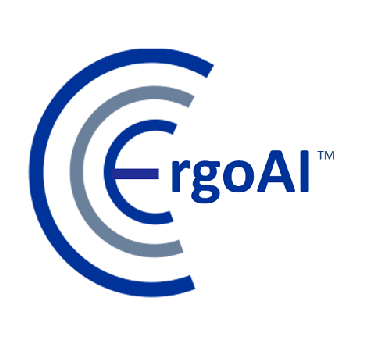
\includegraphics[width=2in]{../etc/ergoAI-bigicon} 
        \vspace{0.7cm}\\
        \Huge A Guide to \ERGOAI Packages
           \vspace{3mm}\\
       {\LARGE Version 3.1 (Arete)}
       }

\author{
  \large Edited by \vspace{3mm}\\
  \Large
  Michael Kifer \vspace{1mm}\\
  \Large
  Coherent Knowledge
  %%\vspace{15mm}\\
  %%\bf
  %%This document contains information proprietary to Coherent Knowledge.\\
  %%\bf
  %%Do not redistribute without authorization from Coherent Knowledge.
  \vspace{2cm}\\
  \monthname ~\the\year
  \vspace{5.3cm}\\
  Portions Copyright $\copyright$ 2013--\the\year{} Coherent Knowledge
}

\date{}

\date{}

\makeindex 
\begin{document}

\pagenumbering{Alph}
\maketitle


\thispagestyle{empty}
\bibliographystyle{plain}
%%\newpage
%%\thispagestyle{empty}

\pagenumbering{roman}
\setcounter{page}{1}
\tableofcontents
\newpage        % Just to avoid a silly LaTeX bug with \pagenumbering
  
\pagenumbering{arabic}



\chapter[JAVA-to-\FLSYSTEM Interfaces]
{JAVA-to-\FLSYSTEM Interfaces\\
  {\Large by Aditi Pandit and Michael Kifer}}


This chapter documents the API for accessing \FLSYSTEM from Java
programs.  The API has two versions: a \emph{low-level API} (used most
commonly), which
enables Java programs to send arbitrary queries to \FLSYSTEM and
get results, and an \emph{experimental}
\emph{high-level API}, which is more limited and requires some setup,
but can simplify a number of tasks in interfacing the two systems. The high-level API establishes a
correspondence between Java classes and \FLSYSTEM classes, which
enables manipulation of \FLSYSTEM classes by executing appropriate
methods on the corresponding Java classes. Both interfaces rely on
the Java-XSB interface, called \emph{Interprolog} \cite{Calejo2004}, developed by
\url{http://interprolog.com/}.

The API assumes that a Java program is started first and then it invokes
XSB/\FLSYSTEM as a subprocess. The XSB/\FLSYSTEM side is passive: it only
responds to the queries sent by the Java side.
Queries can be anything that is accepted at the \FLSYSTEM
shell prompt: queries, insert/delete commands, control switches, etc., are
all fine.
One thing to remember is that the backslash is used in Java
as an escape symbol and in \FLSYSTEM as a prefix of the builtin operators
and commands. Therefore, each backslash must be escaped with another
backslash. That is, instead of a query like "\texttt{p(?X) \bs{}and q(?X).}"
the API requires "\texttt{p(?X) \bs{}\bs{}and q(?X)}.".

\paragraph{The \texttt{FloraObject} object.}
While reading this document one will notice that the class
\texttt{FloraObject} is used in many cases. This class consists of
Java objects that
encapsulate  \FLSYSTEM objects. These Java objects
are mostly used internally.
From the end user's point of view, the only method of interest in this
class is
\texttt{toString()}. 


\section{The Low-level Interface} \label{sec-java-lowlevel}
 The low-level API enables Java programs to send arbitrary queries
to \FLSYSTEM and get results. 
It is assumed that the following two Java properties
are set either as part of the java command (e.g.,  \texttt{java
  ... -DPROLOGDIR=some-dir ...}) or inside the Java application itself, e.g.,
%% 
\begin{verbatim}
System.setProperty("PROLOGDIR","C:\\JSmith\\XSB\\config\\x64-pc-windows\\bin");
\end{verbatim}
%%
Please remember that Windows uses backslash as a file separator, and inside a
Java program these backslashes must be doubled, as shown above.

The two aforementioned properties are:
\begin{description}
\item[\texttt{PROLOGDIR}:] 
This variable points to the folder
containing the XSB executable (binary, not the command script).
\\
To get the right value for your installation, start
\FLSYSTEM and execute this at the prompt:
%% 
\begin{verbatim}
system{bindir = ?D}.
\end{verbatim}
%% 
The result will be returned in the variable \texttt{?D}. 

\item[{\tt FLORADIR}:]
\label{page-floradir}
  This variable must point to the folder
containing the \FLSYSTEM installation.
\\
To get the right value for your installation, start
\FLSYSTEM and execute this at the prompt:
%% 
\begin{verbatim}
system{installdir = ?D}.
\end{verbatim}
%% 
Again, the result will be returned in the variable \texttt{?D}. 
\end{description}
  %%

\bigskip

In order to be able to access \FLSYSTEM, the Java program must first establish
a session for a running instance of \FLSYSTEM. Multiple sessions can be active
at the same time. The knowledge bases in the different running instances
are completely independent. Sessions are instances of
the class {\tt net.sf.flora2.API.FloraSession}. This class provides methods
for opening/closing sessions and loading \FLSYSTEM knowledge bases
(which are also used in the high-level
interface). In addition, a session provides 
methods for executing arbitrary \FLSYSTEM queries. The following is the complete
list of the methods that are available in that class.
All these are \emph{public}
\emph{instance} methods  and the word ``public'' is therefore omitted.
%%
\begin{itemize}
\item
\begin{verbatim}
FloraSession()
\end{verbatim}
  This constructor creates a connection to an instance of \FLSYSTEM.
  Use it like this:
  %% 
\begin{verbatim}
    FloraSession session = new FloraSession();
\end{verbatim}
  %% 
  All the methods below are executed on \texttt{FloraSession}-objects
  produced in this way. 
\item {\tt close()} \\
  This method must be called to terminate a \FLSYSTEM session. Note that this does
  not terminate the Java program that initiated the session:
  to exit the Java program that talks to \FLSYSTEM, one needs to execute
  the statement
  %%
\begin{verbatim}
 System.exit();  
\end{verbatim}
  %%
  Note that just returning from the {\tt main} method is not enough. 

\item
\begin{verbatim}
Iterator<FloraObject> executeQuery(String query)
\end{verbatim}
    This method executes the \FLSYSTEM query given by the
parameter {\tt query}.
The query must be terminated with a period, exactly as it would be typed
in the \FLSYSTEM shell.
It is used to execute \FLSYSTEM queries that
do not require variable bindings to be returned back to Java \emph{or} queries that
have only
a single variable to be returned. Each binding is represented as
an instance of the class {\tt net.sf.flora2.API.FloraSession}.
The examples below illustrate how to process the results returned by this
method.

\item
\begin{verbatim}
Iterator<HashMap<String,FloraObject>> executeQuery(String query,Vector vars)
\end{verbatim}
  This method executes the \FLSYSTEM query given by the first argument.
The query must be terminated with a period, as if it were typed
in the \FLSYSTEM shell.
 The Vector {\tt vars} (of strings) specifies the names of all the variables
  in the query for which bindings need to be returned. These variables are
  added to the vector using the method {\tt add} before calling
  {\tt executeQuery}. For instance, {\tt vars.add("?X")}.  
  
  This version of {\tt executeQuery} returns an iterator over all bindings
  returned by the \FLSYSTEM query.  Each binding is represented by a {\tt
    HashMap<String,FloraObject>} 
  object which can be used to obtain the value of each variable in the
  query (using the {\tt get()} method). The value of each variable returned
  is an instance of {\tt net.sf.flora2.API.FloraObject}.

  The examples below show how to handle the results returned by this method.

\item \texttt{boolean executeCommand(String command)} \\
  This is a simplified way of executing \FLSYSTEM queries that \emph{do not need}
  to return any results, i.e., when the user wants to know if the query is
  true or false for \emph{some} bindings of command's arguments (if there
  are any), but not the actual bindings.
  There are also differences (compared to \texttt{executeQuery()})
  in the way this command handles exceptions, as
  explained in the next section.
  As before, the command must be terminated with a period.

\item
\begin{verbatim}
boolean loadFile(String fileName,String moduleName)
\end{verbatim}
  This method loads the \FLSYSTEM program, specified by the parameter {\tt
    fileName} into the \FLSYSTEM module specified in {\tt moduleName}.
  If errors occur during loading, \texttt{loadFile()} returns \texttt{false}.  
\item
\begin{verbatim}
boolean compileFile(String fileName,String moduleName)
\end{verbatim}
  This method compiles (but does not load)
  the \FLSYSTEM program, specified by the parameter {\tt
    fileName} for the \FLSYSTEM module specified in {\tt moduleName}.
  If errors occur during compilation, \texttt{compileFile()} returns \texttt{false}.  
\item
\begin{verbatim}
boolean addFile(String fileName,String moduleName)
\end{verbatim}
  This method adds the \FLSYSTEM program, specified by the parameter {\tt
    fileName} to an existing \FLSYSTEM module specified in {\tt moduleName}.
  If errors occur during addition, \texttt{addFile()} returns \texttt{false}.  
\item
\begin{verbatim}
boolean compileaddFile(String fileName,String moduleName)
\end{verbatim}
  This method compiles the \FLSYSTEM program, specified by the parameter {\tt
    fileName} for addition to the \FLSYSTEM module specified in {\tt moduleName}.
  If errors occur during compilation, \texttt{compileaddFile()} returns \texttt{false}.  
\end{itemize}

The code snippet below illustrates the low-level API.

\paragraph{Step 1: Writing \FLSYSTEM programs to be called by Java.}
  Let us assume that we have a file, called  {\tt flogic\_basics.flr},
  which contains the following information:
\begin{quote}
\begin{verbatim}
person :: object.
dangerous_hobby :: object.
john:employee.
employee::person.

bob:person.
tim:person.
betty:employee.

person[|age=>integer,
       kids=>person,
       salary(year)=>value,
       hobbies=>hobby,
       believes_in=>something,
       instances => person
|].

mary:employee[
    age->29,
    kids -> {tim,leo,betty},
    salary(1998) -> a_lot
].

tim[hobbies -> {stamps, snowboard}].
betty[hobbies->{fishing,diving}].

snowboard:dangerous_hobby.
diving:dangerous_hobby.

?_X[self-> ?_X].

person[|believes_in -> {something, something_else}|].
\end{verbatim}
\end{quote}

\paragraph{Step 2:  Writing a JAVA application to interface with \FLSYSTEM.}
 The following code loads a \FLSYSTEM program from a file and then passes
 queries to the knowledge base.

\begin{verbatim}
import java.util.*;
import net.sf.flora2.API.*;
import net.sf.flora2.API.util.*;

public class flogicbasicsExample {

    public static void main(String[] args) {
        // create a new session for a running instance of the engine
        FloraSession session = new FloraSession();
        System.out.println("Engine session started");

        // Assume that Java was called with -DINPUT_FILE=the-file-name
        String fileName = System.getProperty("INPUT_FILE");
        if(fileName == null || fileName.trim().length() == 0) {
            System.out.println("Invalid path to example file!");
            System.exit(0);

        }
        // load the program into module basic_mod
        if (session.loadFile(fileName,"basic_mod"))
            System.out.println("Example loaded successfully!");
        else
            System.out.println("Error loading the example!");

        /* Running queries from flogic_basics.flr */

        /* Query for persons */
        String command = "?X:person@basic_mod.";
        System.out.println("Query:"+command);
        Iterator<FloraObject> personObjs = session.executeQuery(command);

        /* Printing out the person names and information about their kids */
        while (personObjs.hasNext()) {
            FloraObject personObj = personObjs.next();
            System.out.println("Person name:"+personObj);
        }

        command = "person[instances -> ?X]@basic_mod.";
        System.out.println("Query:"+command);
        personObjs = session.executeQuery(command);

        /* Printing out the person names  */
        while (personObjs.hasNext()) {
            Object personObj = personObjs.next();
            System.out.println("Person Id: "+personObj);
        }

        /* Example of executeQuery with two arguments */
        Vector<String> vars = new Vector<String>();
        vars.add("?X");
        vars.add("?Y");

        Iterator<HashMap<String,FloraObject>> allmatches =
            session.executeQuery("?X[believes_in -> ?Y]@basic_mod.",vars);
        System.out.println("Query:?X[believes_in -> ?Y]@basic_mod.");
        while(allmatches.hasNext()) {
            HashMap<String,FloraObject> firstmatch = allmatches.next();
            Object Xobj = firstmatch.get("?X");
            Object Yobj = firstmatch.get("?Y");
            System.out.println(Xobj+" believes in: "+?Yobj);
        }
        // quit the system
        session.close();
        System.exit(0);
    }
}
\end{verbatim}

 For the information on how to invoke the above Java class in the context
 of the Java-\FLSYSTEM API,
 please see Section~\ref{sec-executing-apps}.

\section{Debugging \FLSYSTEM Statements Used in a Java Program}

\subsection{Logging}

It often happens that an \FLSYSTEM query or a file used from within a Java
Program has an error and \texttt{executeQuery()} returns an error message
saying that there is a ``problem'' with a \FLSYSTEM statement.
The Java part does not know what the problem is but it can be told to show
the output of the \FLSYSTEM statements on the console. This can be done by
executing the statement
%% 
\begin{verbatim}
    FloraSession.showOutput();
\end{verbatim}
%% 
This will stream all warnings, errors, and just normal output from
\FLSYSTEM to the console.
When no longer needed, this mode can be turned off like this:
%% 
\begin{verbatim}
    FloraSession.hideOutput();
\end{verbatim}
%% 
The \texttt{FloraSession.showOutput();} statement can be executed at any
point in the program, but preferably after calling \texttt{FloraSession()},
to avoid irrelevant output.

Here is an example of what you might see:
%% 
\begin{verbatim}
My command 2 has succeeded

yes

Loading file test.ergo:

yes

++Error[Ergo]> [test.ergo] <Composer> near line(2)/char(3) `b' unexpected operand:
 ',', '.', or some other operator may be missing just before the indicated location

++1 error

++compilation aborted
\end{verbatim}
%% 
Here the output from \FLSYSTEM starts with normal output from, say,
\texttt{writeln(...)@\bs{}io} commands and ends with a compilation error
encountered while compiling the file \texttt{test.ergo}.  
(The above is output from \ERGO; in \FLORA it will be similar.)

Two other useful calls are
%% 
\begin{verbatim}
    FloraSession.enableLogging();
    FloraSession.disableLogging();
\end{verbatim}
%%
Executing \texttt{FloraSession.enableLogging();} will cause the Java API to
record all major events such as starting a session, ending it, loading or
adding a \FLSYSTEM file, and execution of every query. It does not report
query answers, however. Logging can be enabled or disabled anywhere in the
program, but, of course, the log messages will start to appear only after
the enabling command is executed and will cease to appear after
\texttt{disableLogging()} is executed. 

\subsection{Catching Exceptions, Checking Errors and Warnings}

Logging allows one to find errors and warnings in an \FLSYSTEM
subprocess of a Java program by checking the output produced by the session.
However, often one needs to be able to do this \emph{programmatically}  and
this can be done as follows.

\paragraph{Exceptions.} First, if a running \FLSYSTEM query invoked via
\texttt{executeQuery()}
issues a
run-time error, a Java \texttt{FlrException} is thrown, and this can be
caught by the parent Java program.
An exception is also thrown if the query passed to \texttt{executeQuery()}
has a syntax error.\footnote{
  If the query statement itself has no syntax error but it loads a file
  that has a syntax error then \emph{no} exception is thrown. Read on to
  see how to identify this situation programmatically.
}
%% 
Note that \FLSYSTEM statements invoked via 
the other methods (\texttt{executeCommand()},
\texttt{loadFile()}, etc.) do \emph{not} throw  exceptions and errors that
occur during the execution of those statements can be detected only through
the mechanism of \texttt{hasErrors()} described below. 
However, \texttt{executeCommand()}, \texttt{loadFile()},
\texttt{addFile()}, etc., may throw exceptions for other reasons, such as  
a wrong module in \texttt{loadFule()}, etc. 

\paragraph{Detecting syntax errors and warnings.}
Errors and warnings produced
by the \FLSYSTEM compiler do \emph{not} result in exceptions, so they
cannot be caught via Java's try-catch mechanism. To detect if a previous
\texttt{executeQuery()},  \texttt{executeCommand()}, \texttt{loadFile()},
or similar API command produced a warning or an error, use the following
\emph{public} \emph{instance}  methods in class \texttt{FloraSession}:
%% 
\begin{itemize}
\item  \texttt{boolean hasErrors()} --- executing
  \texttt{session.hasErrors()}, where session is a variable holding
  a \texttt{FloraSession}
  object created earlier,
  will tell if a previous \texttt{executeQuery()} or other such
  command (executed on the same \texttt{FloraSession} object)
  has produced an error. This also includes runtime errors, like
  \texttt{FlrException}'s. 
\item  \texttt{boolean hasWarnings()} --- executing
  \texttt{session.hasWarnings()}, where session is a  variable holding
  a \texttt{FloraSession}
  object, will tell if a previous \texttt{executeQuery()} or other such
  command (executed on the same \texttt{FloraSession} object)
  has produced a warning.
\end{itemize}
%% 




\section{The High-Level Interface (experimental)}

The high-level API operates by creating proxy Java classes for 
\FLSYSTEM classes selected by the user.
This enables the Java program to operate on \FLSYSTEM classes by
executing appropriate methods on the corresponding proxy Java classes.
However, compared to the low-level interface, the high-level one is
somewhat limited.  Both interfaces can be used at the same time, if desired.

\textbf{Note A:}  
Most users appear to opt for the low-level interface and such readers
can skip this section.

\textbf{Note B}: This interface will not work for \FLSYSTEM programs that
use \emph{non-alphanumeric} names for methods and predicates. For instance,
if a program involves statements like \texttt{foo['bar\$\#123'->456]} then
the interface might generate syntactically incorrect Java proxy classes and
errors will be issued during the compilation. 

\bigskip

The use of the high-level API involves a number of steps, as described below.

\paragraph{Stage 1: Writing \FLSYSTEM programs to use with the high-level
  interface.}
We assume the same {\tt flogic\_basics.flr} file as in the previous
example.

\paragraph{Stage 2: Generating Java classes that serve as proxies for \FLSYSTEM classes.}
The \FLSYSTEM side of the Java-to-\FLSYSTEM high level API provides a predicate
to generate Java proxy classes for each \fl class which have a signature
declaration in the \FLSYSTEM knowledge base. A proxy class gets defined so
that it would have methods to manipulate the attributes and methods of the
corresponding \fl class for which signature declarations are available.  If
an \fl class has a declared value-returning attribute {\tt foobar} then the
proxy class will have the following methods. Each method name has the form
\emph{action}$S_1S_2S_3$\_{\tt foobar}, where \emph{action} is either {\tt
  get}, {\tt set}, or {\tt delete}. The specifier $S_1$ indicates the type
of the method --- {\tt V} for value-returning, {\tt B} for Boolean, and
{\tt P} for procedural. The specifier $S_2$ tells whether the operation
applies to the signature of the method ({\tt S}), e.g., {\tt
  person[foobar=>string]}, or to the actual data ({\tt D}), for example,
{\tt john[foobar->3]}.  Finally, the specifier $S_3$ tells if the operation
applies to the inheritable variant of the method ({\tt I})
or its non-inheritable variant ({\tt N}).
%% 
\begin{enumerate}
\item {\tt public Iterator<FloraObject> getVDI\_foobar()}\\
  {\tt public Iterator<FloraObject> getVDN\_foobar()}
  \\
  {\tt public Iterator<FloraObject> getVSI\_foobar()}\\
  {\tt public Iterator<FloraObject> getVSN\_foobar()}
  \\
  The above methods query the knowledge base and get all answers for the
  attribute {\tt foobar}. They return iterators through which these answers
  can be processed one-by-one. Each object returned by the iterator is of
  type {\tt FloraObject}.  The {\tt getVDN} form queries non-inheritable
  data methods and {\tt getVDI} the inheritable ones. The {\tt getVSI} and
  {\tt getVSN} forms query the signatures of the attribute {\tt foobar}.
\item {\tt public boolean setVDI\_foobar(Vector value)}\\
  {\tt public boolean setVDN\_foobar(Vector value)}
  \\
  {\tt public boolean setVSI\_foobar(Vector value)}\\
  {\tt public boolean setVSN\_foobar(Vector value)}
  \\
  These methods
  add values to the set of values returned by the attribute {\tt foobar}. The
  values must be placed in the vector parameter passed these methods.
  Again, {\tt setVDN} adds data for non-inheritable methods and {\tt setVDI}
  is used for inheritable methods.
  {\tt setVSI} and {\tt setVSN} add types to signatures.  
\item {\tt public boolean setVDI\_foobar(Object value)}\\
  {\tt public boolean setVDN\_foobar(Object value)}
  \\
  {\tt public boolean setVSI\_foobar(Object value)}\\
  {\tt public boolean setVSN\_foobar(Object value)}\\
  These methods provide a simplified interface when only one value needs to
  be added.  It works like the earlier set\_* methods, except that only one
  value given as an argument is added.
\item {\tt public boolean deleteVDI\_foobar(Vector value)}\\
  {\tt public boolean deleteVDN\_foobar(Vector value)}
  \\
  {\tt public boolean deleteVSI\_foobar(Vector value)}\\
  {\tt public boolean deleteVSN\_foobar(Vector value)}
  \\
  Delete a set of values of the attribute {\tt foobar}. The set is
  specified in the vector argument.
\item {\tt public boolean deleteVDI\_foobar(Object value)}\\
  {\tt public boolean deleteVDN\_foobar(Object value)}
  \\
  {\tt public boolean deleteVSI\_foobar(Object value)}\\
  {\tt public boolean deleteVSN\_foobar(Object value)}
  \\
  A simplified interface for the case when only one value needs to be deleted.
\item {\tt public boolean deleteVDI\_foobar()}\\
  {\tt public boolean deleteVDN\_foobar()}
  \\
  {\tt public boolean deleteVSI\_foobar()}\\
  {\tt public boolean deleteVSN\_foobar()}
  \\
  Delete all values for the attribute {\tt foobar}. 
\end{enumerate}
%% 
For \fl methods with arguments, the high-level API provides Java methods as
above, but they take more arguments to accommodate the parameters that \fl
methods take. Let us
assume that the \fl method is called {\tt foobar2} and it takes parameters
{\tt arg1} and {\tt arg2}.  As before the {\tt getVDI\_*}, {\tt setVDI\_*},
etc., forms of the Java methods are for dealing with inheritable \FLSYSTEM
methods and the {\tt getVDN\_*}, {\tt setVDN\_*},
etc., forms are for dealing with non-inheritable \FLSYSTEM methods.

%%
\begin{enumerate}
\item {\tt public Iterator<FloraObject> getVDI\_foobar2(Object arg1, Object arg2)}\\
  {\tt public Iterator<FloraObject> getVDN\_foobar2(Object arg1, Object arg2)}
  \\
  Obtain all values for the \fl method invocation {\tt foobar2(arg1,arg2)}.
\item {\tt public boolean setVDI\_foobar2(Object arg1, Object arg2, Vector value)}\\
  {\tt public boolean setVDN\_foobar2(Object arg1, Object arg2, Vector value)}
  \\
  Add a set of methods specified in the parameter {\tt value} for the method
  invocation {\tt foobar2(arg1,arg2)}. 
\item {\tt public boolean setVDI\_foobar2(Object arg1, Object arg2, Object value)}\\
  {\tt public boolean setVDN\_foobar2(Object arg1, Object arg2, Object value)}
  \\
  A simplified interface when only one value is to be added.
\item {\tt public boolean deleteVDI\_foobar2(Object arg1, Object arg2, Vector value)}\\
  {\tt public boolean deleteVDN\_foobar2(Object arg1, Object arg2, Vector value)}
  \\
  Delete a set of values from {\tt foobar2(arg1,arg2)}. The set is given by
  the vector parameter {\tt value}. 
\item {\tt public boolean deleteVDI\_foobar2(Object arg1, Object arg2, Object value)}\\
  {\tt public boolean deleteVDN\_foobar2(Object arg1, Object arg2, Object value)}
  \\
  A simplified interface for deleting a single value.
\item {\tt public boolean deleteVDI\_foobar2(Object arg1, Object arg2)}\\
  {\tt public boolean deleteVDN\_foobar2(Object arg1, Object arg2)}
  \\
  Delete all values for the method invocation {\tt foobar2(arg1,arg2)}. 
\end{enumerate}
%% 
For Boolean and procedural methods, the generated methods are similar
except that there is only one version for the set and delete methods. In
addition, Boolean inheritable methods use the {\tt getBDI\_*}, {\tt
  setBDI\_*}, etc., form, while non-inheritable methods use the {\tt
  getBDN\_*}, etc., form.  Procedural methods use the {\tt getPDI\_*}, {\tt
  getPDN\_*}, etc., forms.  For instance,
%% 
\begin{enumerate}
\item  {\tt public boolean getBDI\_foobar3()}   \\
  {\tt public boolean getBDN\_foobar3()} \\
  {\tt public boolean getPDI\_foobar3()}   \\
  {\tt public boolean getPDN\_foobar3()}
\item {\tt public boolean setBDI\_foobar3()}   \\
  {\tt public boolean setBDN\_foobar3()} \\
  {\tt public boolean setPDI\_foobar3()}   \\
  {\tt public boolean setPDN\_foobar3()}
\item {\tt public boolean deleteBDI\_foobar3()}  \\
  {\tt public boolean deleteBDN\_foobar3()}  \\
  {\tt public boolean deletePDI\_foobar3()}  \\
  {\tt public boolean deletePDN\_foobar3()}  
\end{enumerate}
%% 

In addition, the methods to query the ISA hierarchy are available:
%% 
\begin{itemize}
\item  {\tt public Iterator<FloraObject> getDirectInstances()}
\item  {\tt public Iterator<FloraObject> getInstances()}
\item  {\tt public Iterator<FloraObject> getDirectSubClasses()}
\item  {\tt public Iterator<FloraObject> getSubClasses()}
\item   {\tt public Iterator<FloraObject> getSuperClasses()}   
\item   {\tt public Iterator<FloraObject> getDirectSuperClasses()}   
\end{itemize}
%% 
These methods apply to the java proxy object that corresponds to the \fl
class person.

All these methods are generated automatically by executing the following
\FLSYSTEM query (defined in the \texttt{javaAPI} package in \FLSYSTEM).
All arguments in the query must be bound:
%% 
\begin{verbatim}
 // write(?Class,?Module,?ProxyClassFileName).
 ?- write(foo,example,'myproject/foo.java').
\end{verbatim}
%% 
The first argument specifies the class for which to generate the methods,
the file name tells where to put the Java file for the proxy object,
and the model argument tells which \FLSYSTEM model to load this program to. The
result of this execution will be the file {\tt foo.java} which should be
included with your java program (the program that is going to interface with
\FLSYSTEM). Note that because of the Java conventions, the file name must have
the same name as the class name.
It is important to remember, however, that proxy methods will
be generated only for those \fl methods that have been declared using
signatures.

Let us now come back to our program {\tt flogic\_basics.flr} for which we
want to use the high-level API.  Suppose we want to query the person class.
To generate the proxy declarations for that class, we create
the file {\tt person.java} for the 
module {\tt basic\_mod} as follows.
%%
\begin{quote}
\begin{verbatim}
?- load{'examples/flogic_basics'>>basic_mod}.
?- load{javaAPI}.
?- write(person,basic_mod,'examples/person.java')@\prolog
\end{verbatim}
\end{quote}


The {\tt write} method will create the file {\tt person.java} shown
below.  The methods defined in {\tt person.java} are the class constructors
for {\tt person}, the methods to query the ISA hierarchy, and the ``get'',
``set'' and ``delete'' methods for each method and attribute declared in
the \FLSYSTEM class {\tt person}.  The parameters for the ``get'', ``set'' and
``delete'' Java methods are the same as for the corresponding \FLSYSTEM
methods. The first constructor for class {\tt person} takes a low-level
object of class {\tt net.sf.flora2.API.FloraObject} as a
parameter. The second parameter is the \FLSYSTEM module for which the proxy
object is to be created.
The second {\tt person}-constructor takes \fl object Id instead of a
low-level {\tt FloraObject}. It also takes the module name, as before, but,
in addition, it takes a session for a running \FLSYSTEM instance.
The session parameter was not needed for the first {\tt person}-constructor
because {\tt FloraObject} is already attached to a concrete session.  

It can be seen from the form of the proxy object constructors that
proxy objects are attached to specific \FLSYSTEM modules, which may seem to
go against the general philosophy that \fl objects do not belong to any
module --- only their methods do. On closer examination, however, attaching
high-level proxy Java objects to modules makes perfect sense. Indeed, a
proxy object encapsulates operations for manipulating \fl attributes 
and methods, which belong to concrete \FLSYSTEM modules, so the proxy object
needs to know which module it operates upon.


\underline{{\bf person.java file}}

\begin{verbatim}
import java.util.*;
import net.sf.flora2.API.*;
import net.sf.flora2.API.util.*;

public class person {

  public FloraObject sourceFloraObject;

  // proxy objects' constructors
  public person(FloraObject sourceFloraObject, String moduleName){ ... }
  public person(String floraOID,String moduleName, FloraSession session){...}

  // ISA hierarchy queries
  public Iterator<FloraObject> getDirectInstances() { ... }
  public Iterator<FloraObject> getInstances() { ... }
  public Iterator<FloraObject> getDirectSubClasses() { ... }
  public Iterator<FloraObject> getSubClasses() { ... }
  public Iterator<FloraObject> getDirectSuperClasses() { ... }
  public Iterator<FloraObject> getSuperClasses() { ... }

  // Java methods for manipulating methods
  public boolean setVDI_age(Object value) { ... }
  public boolean setVDN_age(Object value) { ... }
  public Iterator<FloraObject> getVDI_age(){ ... }
  public Iterator<FloraObject> getVDN_age(){ ... }
  public boolean deleteVDI_age(Object value) { ... }
  public boolean deleteVDN_age(Object value) { ... }
  public boolean deleteVDI_age() { ... }
  public boolean deleteVDN_age() { ... }
  public boolean setVDI_salary(Object year,Object value) { ... }
  public boolean setVDN_salary(Object year,Object value) { ... }
  public Iterator<FloraObject> getVDI_salary(Object year) { ... }
  public Iterator<FloraObject> getVDN_salary(Object year) { ... }
  public boolean deleteVDI_salary(Object year,Object value) { ... }
  public boolean deleteVDN_salary(Object year,Object value) { ... }
  public boolean deleteVDI_salary(Object year) { ... }
  public boolean deleteVDN_salary(Object year) { ... }
  public boolean setVDI_hobbies(Vector value) { ... }
  public boolean setVDN_hobbies(Vector value) { ... }
  public Iterator<FloraObject> getVDI_hobbies(){ ... }
  public Iterator<FloraObject> getVDN_hobbies(){ ... }
  public boolean deleteVDI_hobbies(Vector value) { ... }
  public boolean deleteVDN_hobbies(Vector value) { ... }
  public boolean deleteVDI_hobbies(){ ... }
  public boolean deleteVDN_hobbies(){ ... }
  public boolean setVDI_instances(Vector value) { ... }
  public boolean setVDN_instances(Vector value) { ... }
  public Iterator<FloraObject> getVDI_instances(){ ... }
  public Iterator<FloraObject> getVDN_instances(){ ... }
  public boolean deleteVDI_instances(Vector value) { ... }
  public boolean deleteVDN_instances(Vector value) { ... }
  public boolean deleteVDI_instances(){ ... }
  public boolean deleteVDN_instances(){ ... }
  public boolean setVDI_kids(Vector value) { ... }
  public boolean setVDN_kids(Vector value) { ... }
  public Iterator<FloraObject> getVDI_kids(){ ... }
  public Iterator<FloraObject> getVDN_kids(){ ... }
  public boolean deleteVDI_kids(Vector value) { ... }
  public boolean deleteVDN_kids(Vector value) { ... }
  public boolean deleteVDI_kids(){ ... }
  public boolean deleteVDN_kids(){ ... }
  public boolean setVDI_believes_in(Vector value) { ... }
  public boolean setVDN_believes_in(Vector value) { ... }
  public Iterator<FloraObject> getVDI_believes_in(){ ... }
  public Iterator<FloraObject> getVDN_believes_in(){ ... }
  public boolean deleteVDI_believes_in(Vector value) { ... }
  public boolean deleteVDN_believes_in(Vector value) { ... }
  public boolean deleteVDI_believes_in(){ ... }
  public boolean deleteVDN_believes_in(){ ... }
}
\end{verbatim}

\paragraph{Stage 3: Writing Java applications that use the high-level API.}

The following program ({\tt flogicbasicsExample.java}) shows several
queries that use the high-level interface. The
class {\tt person.java} is generated at the previous stage.
The methods of the high-level interface operate on Java objects that are
proxies for \FLSYSTEM objects. These Java objects are members of the class
{\tt net.sf.flora2.API.FloraObject}.
Therefore, before one can use the high-level methods one need to first
retrieve the appropriate proxy objects on which to operate. This is done
by sending an appropriate query through the method {\tt executeQuery}---the
same method that was used in the low-level interface.
Alternatively, {\tt person}-objects could be constructed using the
3-argument proxy constructor, which takes \fl oids.


\begin{verbatim}
import java.util.*;
import net.sf.flora2.API.*;
import net.sf.flora2.API.util.*;

public class flogicbasicsExample {

   public static void main(String[] args) {
     /* Initializing the session */
     FloraSession session = new FloraSession();
     System.out.println("Flora session started");

     String fileName = "examples/flogic_basics"; // must be a valid path
     /* Loading the flora file */
     if (session.loadFile(fileName,"basic_mod"))
         System.out.println("Example loaded successfully!");
     else
         System.out.println("Error loading the example!");

     // Retrieving instances of the class person through low-level API
     String command = "?X:person@basic_mod.";
     System.out.println("Query:"+command);
     Iterator<FloraObject> personObjs = session.executeQuery(command);

     /* Print out person names and information about their kids */
     person currPerson = null;
     while (personObjs.hasNext()) {
         FloraObject personObj = personObjs.next();
         // Elevate personObj to the higher-level person-object
         currPerson =new person(personObj,"basic_mod");

         /* Set that person's age to 50 */
         currPerson.setVDN_age("50");

         /* Get this person's kids */
         Iterator<FloraObject> kidsItr = currPerson.getVDN_kids();
         while (kidsItr.hasNext()) {
             FloraObject kidObj = kidsItr.next();
             System.out.println("Person: " + personObj + " has kid: " +kidObj);

             person kidPerson = null;
             // Elevate kidObj to kidPerson
             kidPerson = new person(kidObj,"basic_mod");

             /* Get kidPerson's hobbies */
             Iterator<FloraObject> hobbiesItr = kidPerson.getVDN_hobbies();
             while(hobbiesItr.hasNext()) {
                 FloraObject hobbyObj = hobbiesItr.next();
                 System.out.println("Kid:"+kidObj + " has hobby:" +hobbyObj);
             }
         }
     }

     FloraObject age;
     // create a person-object directly by supplying its F-logic OID
     // father(mary)
     currPerson = new person("father(mary)", "example", session);
     Iterator<FloraObject> maryfatherItr = currPerson.getVDN_age();
     age = maryfatherItr.next();
     System.out.println("Mary's father is " + age + " years old");

     // create a proxy object for the F-logic class person itself
     person personClass = new person("person", "example", session);
     // query its instances through the high-level interface
     Iterator<FloraObject> instanceIter = personClass.getInstances();
     System.out.println("Person instances using high-level API:");
     while (instanceIter.hasNext())
         System.out.println("    " + instanceIter.next());
        
     session.close();
     System.exit();
   }
}
\end{verbatim}

\section{Executing Java Application Programs that Call \FLSYSTEM}
\label{sec-executing-apps}

To compile and run Java programs that interface with \FLSYSTEM, follow the
following guidelines.

\begin{itemize}
\item \emph{Compilation}:
  Place the files {\tt flogicsbasicsExample.java} (the program you have
  written) and {\tt person.java} (the automatically generated file)
in the same directory and compile them using the {\tt javac}  command. Add
the jar-files containing the API code and
{\tt interprolog.jar}  to the classpath using the \texttt{-classpath}
parameter (the first line is for Windows and the second for Mac and Linux):
%% 
\begin{verbatim}
-classpath "%FLORADIR%\java\flora2java.jar";"%FLORADIR%\java\interprolog.jar"
-classpath "$FLORADIR/java/flora2java.jar":"$FLORADIR/java/interprolog.jar"
\end{verbatim}
%% 
\texttt{FLORADIR} here is a shell (cmd, in Windows) variable that can be
set by the 
scripts \texttt{flora\_settings.sh} (Linux/Mac) or \texttt{flora\_settings.bat}
(Windows).
In sum, the Java compilation command should look as below
(again, the first command below is for
Windows and the second for Linux/Mac):
%% 
\begin{alltt}
\emph{path-to}\bs{}javac -classpath
     "%FLORADIR%\bs{}java\bs{}flora2java.jar";"%FLORADIR%\bs{}java\bs{}interprolog.jar"
\emph{path-to}/javac -classpath
     "$FLORADIR/java/flora2java.jar":"$FLORADIR/java/interprolog.jar"
\end{alltt}
%% 
\textbf{Note}: each of the above commands should be on one line.


\item \emph{Running}:  Generally, Java programs that call \FLSYSTEM
  should be invoked using the following command. For 
  Linux and Mac, change \texttt{\%}\textit{VAR}\texttt{\%} to
      \texttt{\$}\textit{VAR}:
\begin{alltt}
\emph{path-to}\bs{}java -DPROLOGDIR=%PROLOGDIR%
                -DFLORADIR=%FLORADIR%
                -Djava.library.path=%PROLOGDIR%            <--- \emph{optional}
                -classpath %MYCLASSPATH% flogicbasicsExample
\end{alltt}
%%
The above commands use several shell/cmd variables that are explained below.
Instead of using the variables, one can substitute their values
directly---read on.

\begin{itemize}
  \item
    If the \texttt{javac} and \texttt{java} commands can be found through
    the \texttt{PATH} environment variable then one can simply type
    \texttt{javac} and \texttt{java} instead of the above.
    On Linux and Mac this is almost always the case, but on Windows one
    might have to set the \texttt{PATH} variable explicitly. 

\item
  {\tt PROLOGDIR}: This variable should point to the directory containing
  the XSB executable, which can be accomplished by executing the scripts
  \texttt{\ENGINENAMEALT\bs{}java\bs{}flora\_settings.bat} (Windows) or
  \texttt{\ENGINENAMEALT/java/flora\_settings.sh} (Linux/Mac).
  \\
  Alternatively, one can type
  \texttt{-DPROLOGDIR=}\emph{path-to-prolog-bindir}
  in the above \texttt{java} command, where the value to substitute for
  \emph{path-to-prolog-bindir} can be obtained 
  by executing this query at the prompt:
%% 
\begin{verbatim}
    system{bindir = ?D}.
\end{verbatim}
%% 
The result will be returned as a binding for the variable \texttt{?D}. 

\item
{\tt FLORADIR}: This variable should be set to the directory
containing the \FLSYSTEM system, which can be done by
executing the aforesaid scripts
\texttt{flora\_settings.bat} and \texttt{flora\_settings.sh}.
\\
Alternatively, one can type
\texttt{-DFLORADIR=}\emph{path-to-flora-dir}
  in the above \texttt{java} command, where the value to substitute for
  \emph{path-to-flora-dir} can be obtained 
  by executing this query at the prompt:
%% 
\begin{verbatim}
    system{installdir = ?D}.
\end{verbatim}
%% 
Again, the result will be returned as a binding of the variable \texttt{?D}. 

\item
{\tt MYCLASSPATH}: This variable should include the correct paths to the
jar files
containing the API code, i.e., \texttt{flora2java.jar} 
and file {\tt interprolog.jar}, plus the directory where the
main application class (like
\texttt{flogicbasicsExample} in our example) is found. 
Normally, one sets \texttt{MYCLASSPATH} to
\texttt{\small\%CLASSPATH\%;\%FLORADIR\%\bs{}java\bs{}flora2java.jar;\%FLORADIR\%\bs{}java\bs{}interprolog.jar;\\DirOfTheExample},
where \texttt{DirOfTheExample} is the directory where the main application
class resides.
In our example, this directory is
simply . (the current directory).
For Linux and Mac, use ':' instead of ';' as a separator, forward slashes
instead of backward ones, and \emph{\$VAR} 
instead of \emph{\%VAR\%}.

One can, of course, substitute the contents of the \texttt{MYCLASSPATH}
variable directly into the \texttt{-classpath \%MYCLASSPATH\%} part of the
above Java/Javac invocation commands.   

\item
The variable \texttt{java.library.path} in the above command  is
optional. It needs to be
set \emph{only if XSB is configured to use the native Java interface} (which
usually is not the case).
\end{itemize}

\item
Some Java applications may employ additional Java properties. For instance,
the program that uses the low-level API in
Section~\ref{sec-java-lowlevel} (in Step 2) has the line 
%% 
\begin{alltt}
      String fileName = System.getProperty("INPUT\_FILE"); 
\end{alltt}
%% 
which means that it expects the property \texttt{INPUT\_FILE} to be set
with the \texttt{-D} option at the Java invocation time.
In general, such additional properties can be also set via the method
\texttt{System.setProperty()} inside the Java application.  
In our particular case, the program expects that \texttt{INPUT\_FILE} is set
to point to
the \texttt{flogic\_basics.flr} \FLSYSTEM file, which it then
loads. In other words, the \texttt{java}  command shown above also needs this
parameter:
%% 
\begin{alltt}
      -DINPUT_FILE="%INPUT\_FILE%"   (Windows)
      -DINPUT_FILE="$INPUT\_FILE"    (Linux/Mac)
\end{alltt}
%% $
In general, one such additional parameter is needed for each property
that the Java application queries using the \texttt{getProperty()} method. 
\end{itemize}

\section{How Do Applications Find  the Knowledge Base?}

When a Java application starts \FLSYSTEM, the latter determines the default
runtime directory in which it will work. Usually, this is the directory in
which your Java application runs. You can find out which directory
it is by sending the following query to \FLSYSTEM:
%% 
\begin{verbatim}
    File[cwd->?Dir]@\io.
\end{verbatim}
%% 
\texttt{?Dir} will be bound to the runtime directory and Java can get that
value as explained earlier. Your Java application can change that
directory via this query:
%% 
\begin{verbatim}
    File[chdir('....new current dir...')]@\io.
\end{verbatim}
%% 
The simplest basic rule is that all \FLSYSTEM's files that your Java
application loads, adds, etc., must be specified relative to the current
directory.

One can also put additional directories to the \FLSYSTEM's search path by
executing the query
%% 
\begin{verbatim}
    Libpath[add('....new dir to search...')]@\sys.
\end{verbatim}
%% 
Then your application can use file names not only relative to the runtime
directory but also relative to any of the directories added in this way.
Note that this may put many directories on the search path, and
several of them may have similarly named files. Therefore,
one must make sure that the search is unambiguous.


\section{Summary of the Variables and Properties Used by the Interface}

The Java-\FLSYSTEM interface needs the following variables and properties
to be set:
%% 
\begin{itemize}
\item  \texttt{JAVA\_HOME} -- this is an OS environment variable.
  It is normally set when you install Java. Normally, Java will not work
  correctly if this environment variable is not set correctly.
%%\item \texttt{MYCLASSPATH}: This variable should point to the jar files
%%containing the API code, i.e., \texttt{.../java/flora2java.jar} 
%%and file {\tt .../java/interprolog.jar}.
\item  The following Java properties must be set for the Java API to work.
  They can be set either through the
  \texttt{-D} option of the \texttt{java} command or inside the Java
  application via \texttt{System.setProperty("propertyname",value)}.  
  %% 
  \begin{itemize}
  \item  \texttt{FLORADIR} --- the path to the \FLSYSTEM installation directory.
  \item  \texttt{PROLOGDIR} --- the path to the folder containing XSB executable.
  \end{itemize}
  %% 
  The proper values for these properties can be obtained from \FLSYSTEM by
  running these queries, respectively:
  %% 
\begin{verbatim}
    system{installdir=?D}.  
    system{bindir=?D}.  
\end{verbatim}
  %% 
\item The following shell/cmd variable is useful, if you do not know where
  the \texttt{java} and \texttt{javac} executables are on your machine.
  This may be needed on Windows, if your JDK installer failed to set the
  Windows \texttt{PATH} environment variable so that the system would find
  these commands easily. (On Linux and Mac the above commands
  are usually fund through the \texttt{PATH} variable.)
  %% 
  \begin{itemize}
  \item   \texttt{JAVA\_BIN} --- the directory where Java executables
    \texttt{java}  and \texttt{javac}  live. It is usually set to \texttt{\$JAVA\_HOME/bin} or
    \texttt{\%JAVA\_HOME\%\bs{}bin}, depending on the OS. 
  \end{itemize}
  %% 
  This variable can be set by
  \texttt{unixVariables.sh} or \texttt{windowsVariables.bat}, whichever
  applies to your OS.
\end{itemize}
%% 

\section{Building the Prepackaged Examples}

Sample applications of the Java-\FLSYSTEM interface
are found in the {\tt java/API/examples}  folder of the \FLSYSTEM
distribution.
%%To build the code for the interface, use the scripts {\tt build.bat} or
%%{\tt build.sh} (or \texttt{build.bat} on Windows)
%%in the {\tt java/API}  folder.
To build the examples, use the scripts
{\tt buildExample.sh} or  {\tt buildExample.bat} in the {\tt java/API/examples}
folder, whichever applies. For instance, to
build the {\tt flogicbasicsExample} example, use these commands on Linux,
Mac, and other Unix-like systems:
%%
\begin{verbatim}
    cd examples
    buildExample.sh flogicbasicsExample
\end{verbatim}
%%
On Windows, use this:
%%
\begin{verbatim}
    cd examples
    buildExample.bat flogicbasicsExample
\end{verbatim}
%%

To run the demos, use the scripts
{\tt runExample.sh} or  {\tt runExample.bat}  in {\tt java/API/examples}.
For instance, to
run the {\tt flogicbasicsExample},  use this command on Linux and Mac:
%%
\begin{verbatim}
    runExample.sh flogicbasicsExample
\end{verbatim}
%%
On Windows, use this:
%%
\begin{verbatim}
    runExample.bat flogicbasicsExample
\end{verbatim}
%%


%%% Local Variables: 
%%% mode: latex
%%% TeX-master: "ergo-packages"
%%% End: 

\chapter[\ERGO-to-Java Interface]
{\ERGO-to-Java Interface: Calling Java from \ERGO\\
  {\Large by Michael Kifer}}


This chapter describes the API for opening some standard Java widgets from
within \ERGO rules. This API also allows one to call arbitrary Java
programs and thereby use \ERGO for scripting Java applications.

The \ERGO-to-Java API works both when \ERGO runs as a standalone
application and when it is under the control of Ergo Studio.
The API calls should work the same in either environment.

\section{General}

The \ERGO-to-Java API is available in the system module \texttt{\bs{}e2j}
and calling anything in this module will load that module. If, however, for
some reason it is necessary to load this module without executing any
operations, one can accomplish this by calling 
%% 
\begin{itemize}
\item  \texttt{ensure\_loaded@\bs{}e2j}. 
\end{itemize}
%% 

The following additional general API calls are available:
%% 
\begin{itemize}
\item  \texttt{System[mode->?Mode]@\bs{}e2j} - the variable \texttt{?Mode} will be bound to one
  of the following:
  %% 
  \begin{itemize}
  \item    \texttt{studio} -- if \ERGO runs as part of Ergo Studio.
  \item    \texttt{[ergo2java,gui]} -- if \ERGO runs as a standalone mode
    in an environment that supports graphics. This is usually the case when
    one invokes \ERGO in a command window on a personal computer.
  \item \texttt{[ergo2java,nogui]} -- this is usually the case when \ERGO
    runs in a non-graphical environment, such as a dumb terminal or a
    command window opened on a remote server.
    In a \texttt{nogui} situation, none of the widgets (windows, dialogs,
    etc.) will be available. However, the dialog boxes will be simulated
    through a command-line interface.
  \end{itemize}
  %% 
  \item \texttt{System[restart]@\bs{}e2j} -- restarts the Java subprocess, if it was
    killed and is needed again. This is required very rarely: for instance,
    when the Java subprocess was killed outside of \ERGO (e.g., via the Task
    Manager or System Monitor). Java is also killed when
    \texttt{\bs{}end} is executed at the \ERGO prompt.
  \item \texttt{System[path(studioLogFile)->?File]@\bs{}e2j} -- also a rarely used
    feature. The variable \texttt{?File} gets
    bound to the location of the Studio log file. This calls fails outside
    of the studio environment. In the future, this API call will be extended
    to include other file locations that might be deemed useful in the
    future.
\end{itemize}
%% 

\section{Dialog Boxes}

This part of the API allows the user to pop up various dialog boxes and
find out which button was clicked by the user. Several types of dialog
boxes are supported:
%% 
\begin{itemize}
\item \texttt{Dialog[show(?Question)->?Answer]@\bs{}e2j} -- pops up a dialog box
  that asks the user a question and provides
  an input text field plus the buttons \texttt{OK} and
  \texttt{Cancel}.   
  If the user clicks \texttt{Cancel} the call fails. Otherwise, if
  \texttt{OK} is clicked, \texttt{?Answer} gets bound to whatever the user
  typed in the input field.   
\item
  \texttt{Dialog[showOptions(?Title,?Message,?Buttons)->?ChosenButton]@\bs{}e2j} --
  opens up a dialog box where the user is presented with a number of
  buttons to click on. Here \texttt{?Title} must be bound to an atom---it
  will be the title of the window;  \texttt{>Message} is an atom that
  contains the message to be displayed to the user (e.g., ``Please click a
  suitable button''); and \texttt{?Buttons} is a list of labels to appear
  on the buttons presented as the available choices (e.g.,
  \texttt{[Milk,Bread,Honey]}).
\item \texttt{Dialog[show(?Title,?Message)]@\bs{}e2j} -- pops up a dialog box that 
  shows a message (\texttt{?Message}) and waits until the user clicks
  \texttt{OK}.  \texttt{?Title} is the title of the dialog box.
\item \texttt{Dialog[chooseFile->?File]@\bs{}e2j} -- pops up a file
  chooser. \texttt{?File} gets bound to the file chosen by the user.
\item \texttt{Dialog[chooseFile(?ExtensionsList)->?File]@\bs{}e2j} -- like the above, but
  also takes a parameter that represents a \emph{list} of  file
  extensions. Only the files
  with that extensions mentioned in the list are shown to the user in the
  file chooser.
\end{itemize}
%% 

\section{Windows}

This part of the API supports opening, closing, and other operations on windows.
%% 
\begin{itemize}
\item \texttt{Window[open(?WindTitle,?Tooltip)->?Window]@\bs{}e2j} -- pops up a new
  window with the title \texttt{?WindTitle} and the tooltip
  \texttt{?Tooltip}. The tooltip is appears when the mouse rests over the
  window. The variable \texttt{?Window} gets bound to the Id of the newly
  created window. This Id will need to be passed to other API calls that
  manipulate windows, so the user must usually store these Ids in some
  predicates.
\item \texttt{Window[setSize(?Win,?Columns,?Rows)]@\bs{}e2j} -- changes the size of
  the window so it will have the given number of columns and rows.
  The system will then try to adjust the window (whose Id is passed in the
  first argument \texttt{?Win}) to approximate the requested size.
\item \texttt{Window[close(?Window)]@\bs{}e2j} -- closes the specified window.
\item \texttt{Window[alive(?Window)]@\bs{}e2j} -- tells if the window is alive
  (i.e., not closed by the user---either programmatically or by clicking
  the \texttt{x} button in the corner of the window). 
\end{itemize}
%% 

\section{Printing to a Window}

The following describes how to print to a previously open window and how to
erase the window contents.
%% 
\begin{itemize}
\item  \texttt{Window[clear(?Window)]@\bs{}e2j} -- erases the contents of the given
  window. 

\item \texttt{Window[print(?Window,?Text)]@\bs{}e2j} -- prints \texttt{?Text} to a
  given window.  \texttt{?Text} specifies what to print and how. Several
  colors are supported (\texttt{black}, \texttt{red}, \texttt{brown},
  \texttt{green}, \texttt{purple}, \texttt{blue}, \texttt{magenta},
  \texttt{orange}, and \texttt{default}), as well as a few faces
  (\texttt{italic}, \texttt{bold}, \texttt{boldital}).

  \texttt{?Text} is either a \emph{text descriptor} or a \emph{list} of
  text descriptors, where a text descriptor is
  %% 
  \begin{itemize}
  \item  a Hilog term; or
  \item  \emph{modifier}(Hilog term)
  \end{itemize}
  %% 
  Here \emph{modifier} is one of the aforesaid colors or faces.
  Not all faces may be available for the default fonts on your system
  so, say, \texttt{boldital} may appear as \texttt{italic} ot as
  \texttt{bold}. Likewise, colors may look different on different screens.   

  Note that
  if you want to print a term like \texttt{red(tomato)} then you would have
  to wrap it in one of the above modifiers, like
  \texttt{default(red(tomato))} (to print \texttt{red(tomato)}  in the default
  color---usually black) or \texttt{green(red(tomato))} (to print
  {\color{green}\texttt{red(tomato)}}). Otherwise, if \texttt{red(tomato)}
  is not wrapped as described, 
  \texttt{{\color{red}tomato}}  will be printed instead.

  Examples. Let us assume that window with Id 3 is open. Then:\\
  \texttt{Window[print(3,magenta('this is red(herring), 1lb'))]@\bs{}e2j}
  will print
  {\color{magenta}this is red(herring), 1lb}.\\
   \texttt{Window[print(3,[magenta('this is a '), green(2),
       italic(' pound '), red(herring)])]@\bs{}e2j}
     will print: {\color{magenta}this is a} {\color{green}2} \emph{pound}
     {\color{red}herring}. 
\end{itemize}
%% 


\section{Scripting Java Applications}

The java scripting API allows the user to load Java jar-files, invoke
methods that exist in the public classes of those jar-files, and process
the results.

%% 
\begin{itemize}
  %% addJar is deprecated
  %% \item  \texttt{System[addJar(?Jar)]@\bs{}e2j} -- load the specified
  %%   jar-file into the system. This API call works with Java 8, but not Java 9+.
\item \texttt{System[setJavaCP(\textnormal{\emph{Classpath}})]@\bs{}e2j} --
  specify the class path for additional Jars and classes to be used at run
  time. \emph{Classpath} must be an atom that represents a valid
  specification for the Java \texttt{-classpath} option.  Note that on
  Windows the elements of a classpath are separated with a ``;'' and on
  Linux/Mac with a ``:''.  Typically this call is made before issuing any
  other calls to \texttt{\bs{}e2j}.  If this is called after some calls to
  \texttt{\bs{}e2j} were issued, the existing Java process is killed first
  and any in-memory data that it may have
  created (e.g., objects that were created) will be discarded.
\item
  \texttt{\textnormal{\emph{JavaObjSpec}}[message(\textnormal{\emph{JavaMethodWithArgs}})
    -> \textnormal{\emph{Result}}]@\bs{}e2j} -- invoke Java method on a
  Java object and return the result.
  \\
  This feature is \emph{experimental} and incomplete. It does not support
  all Java data structures and not all kinds of methods can be applied. 
\end{itemize}
%% 
\emph{JavaObjSpec} in the above \texttt{message(...)}   API can have several forms:
%% 
\begin{itemize}
\item  \texttt{oid(}\emph{Integer}\texttt{)}: When Java returns an object,
  it is registered by \FLSYSTEM and is represented by an integer, e.g.,
  345. In order to 
  invoke a Java method on it, the \emph{JavaObjSpec} must be specified as
  \texttt{oid(345)}.
\item If \emph{JavaObjSpec} is an integer, float, or atom in \ERGO then
  it is interpreted as a Java long, double, or string, respectively. Java
  methods that apply can be used in \texttt{JavaMethodWithArgs}. For instance,
  %% 
\begin{verbatim}
?- '123abc789'[message(split(abc))->?P]@\e2j.
?P = ['123', '789']
?- abc23op[message(matches('.+23.*'))->?P]@\e2j.
?P = \true
?- abcdf[message(getBytes)->?R]@\e2j.
?R = "abcdf"^^\charlist
\end{verbatim}
  %% 
\item If \emph{JavaObjSpec} is a list, it is interpreted as an array of
  objects. For instance, the list \texttt{[pp,i(8),k(u,m)]} is mapped into
  a Java array and \texttt{[1]} is a method applied to that array, which
  returns the second element.  
  %% 
\begin{verbatim}
?- [pp,i(8),k(u,m)][message([1])->?P]@\e2j.
?P = i(8)  
?- [pp,i(8),k(u,m)][message(length)->?P]@\e2j.
?P = 3
\end{verbatim}
  %% 
\item If \emph{JavaObjSpec} is \texttt{byte(}\emph{smallNumber}\texttt{)},
  \texttt{short(}\emph{shortinteger}\texttt{)},
  or \texttt{int(}\emph{integer}\texttt{)}
  then it is interpreted as a byte or int constant.
\item If \emph{JavaObjSpec} is \texttt{term(}\emph{someHiLogTerm}\texttt{)} 
  then \emph{someHiLogTerm} is mapped into a \texttt{TermModel} object---see
  \url{http://interprolog.com/ipjavadoc/com/declarativa/interprolog/TermModel.html}
  for the details of this class, which has methods to de/compose terms on
  the Java side.
  %% 
\begin{verbatim}
?- term(p(a,b))[message(getFunctorArity)->?P]@\e2j.
?P = 'p/2'
\end{verbatim}
  %% 
\item If \emph{JavaObjSpec} is of the form
  \texttt{array(}\emph{type},\emph{list}\texttt{)} then this is mapped to
  an array of constants of the given type (string, byte, int, float). For
  instance
  %% 
\begin{verbatim}
?- array(int,[2,7,99])[message([2])->?P]@\e2j.
?P = 99
\end{verbatim}
  %% 
\item If \emph{JavaObjSpec} is of the form \emph{Wrap(const)}, where
  \emph{Wrap} is one of Boolean, Character, Byte, Double, Float,
  Integer, Long, or Short and \emph{const} is of the appropriate \ERGO
  type, then this will be mapped into an object of type
  \texttt{java.lang.Boolean}, \texttt{java.lang.Character}, etc., respectively.
  Note that these are objects, while the wrappers \texttt{int},
  \texttt{short}, \texttt{byte}, etc., which we introduced earlier   
  are non-object constants.
\item Additionally, to be able to execute \emph{static methods}, fully-qualified
  classes wrapped with \texttt{class} can be used. For instance,
  %% 
\begin{verbatim}
?- class('java.lang.String')[message(format('abc=%d %s',12,iiii))->?R]@\e2j.
?R = 'abc=12 iiii'
?- class('java.lang.String')
              [message(String(array(byte,[119,111,114,108,100])))->?P]@\e2j.
?P = world
\end{verbatim}
  %% 
  \item It is further possible to send a message to a \emph{static variable}
    (i.e., invoke a method on the object held by that static variable, as
    in \texttt{java.lang.System.out.println("Hello")}) 
    in a class as follows:
    %% 
\begin{verbatim}
?- class('java.lang.System'+out)[message(println(Hello))->?R]@\e2j.
Hello
?R = \@?   // a null value because println returns void
?- class('java.lang.System'+out)[message(printf('%1.16g', 69.1))->?R]@\e2j.
69.10000000000000
?R = oid(1)    
\end{verbatim}
    %% 
    Note that here \texttt{out} is the static variable in class
    \texttt{java.lang.String} to which the messages are being sent.  

    Currently it is not possible to get the value of a static variable
    unless there is a getter-method for that variable.
\end{itemize}
%% 
The same mapping conventions are applied to the arguments of the
method-expressions passed to \texttt{message(...)} in our API call. 



%%% Local Variables: 
%%% mode: latex
%%% TeX-master: "../ergo-packages"
%%% End: 

\chapter[Python-to-\ERGO Interface]
{pyergo: A Python-to-\ERGO Interface \\ 
  {\Large by Michael Kifer}}

This interface allows Python programs to start \ERGO, load knowledge bases
into it, and then query and modify them.  One can also talk directly to the
underlying Prolog engine, XSB.
This API works both with Python 2.7 and 3.X, but 3.7+ is recommended.

\section{Introduction}

The \emph{pyergo} interface consists of four types of APIs: one for
starting and closing \ERGO sessions, one for querying \ERGO,
one for talking directly to XSB, and one for parsing the results.
A fairly extensive example of a program that does both is found in
%% 
\begin{verbatim}
    .../ErgoAI/python/pyergo_example.py
\end{verbatim}
%% 
in the \ERGO distribution. This program provides several examples of using
the \texttt{pyergo} interface, including various edge cases and exception
handling. 
The easiest way to try these examples is via the provided shell scripts,
%% 
\begin{verbatim}
    .../ErgoAI/python/runpyergo.sh    -- Linux/Mac
    .../ErgoAI/python/runpyergo.bat   -- Windows
\end{verbatim}
%% 
One only has to change the two variables in those scripts \texttt{ERGOROOT}
and \texttt{XSBARCHDIR}.

To make it possible for your Python program
find \ERGO, two parameters are to be provided: the architecture directory,
called \texttt{XSBARCHDIR} in those scripts and in
\texttt{pyergo\_example.py}, and the root directory for the \ERGO reasoner,
which we called \texttt{ERGOROOT}. The names of these variables are, of
course immaterial, but we will use these names here for easy reference.
Pay attention to how this information is passed from the scripts to the
program via the \texttt{sys.argv}  array, as this is one of the most
convenient methods.

How will you know what to substitute for the aforesaid \texttt{ERGOROOT}
and \texttt{XSBARCHDIR}? Easy! Just start \ERGO and type these two
queries:
%% 
\begin{verbatim}
    ?- system{installdir=?Ins}.  // gives ERGOROOT
    ?- system{archdir=?Arch}.    // yields XSBARCHDIR
\end{verbatim}
%% 
The first query will give you \texttt{ERGOROOT} and the second
\texttt{XSBARCHDIR}.

Next your program needs to be told where the interface can be found. In our
example, this is accomplished via
%% 
\begin{verbatim}
    import sys
    sys.path.append(ERGOROOT.replace('\\','/') + '/python')
\end{verbatim}
%% 
Of course, you will have to replace \texttt{ERGOROOT} here appropriately,
as explained.
Note that forward slashes are preferred, although backward slashes are also
recognized in Windows (sometimes they must be escaped with another
backslash to satisfy Python syntax).
Finally, import the API as follows:
%% 
\begin{alltt}
from pyergo import \bs
    pyergo_start_session, pyergo_end_session, \bs  \emph{\color{blue}to start/end Ergo session}
    pyergo_command, pyergo_query,            \bs   \emph{\color{blue}to talk to Ergo}
    HILOGFunctor, PROLOGFunctor,             \bs   \emph{\color{blue}to parse results from Ergo}
    ERGOVariable, ERGOString, ERGOIRI, ERGOSymbol, \bs
    ERGOIRI, ERGOCharlist, ERGODatetime,     \bs
    ERGODuration, ERGOUserDatatype,          \bs
    pyxsb_query, pyxsb_command,              \bs   \emph{\color{blue}to talk to XSB directly}
    XSBFunctor, XSBVariable, XSBAtom,        \bs   \emph{\color{blue}to parse results from XSB}
    XSBString,                               \bs
    PYERGOException, PYXSBException              \emph{\color{blue}to process exceptions}
\end{alltt}
%% 
In most cases you will need only a small subset of these functions, but
importing them all is easy, does not hurt,
and is useful in case you later extend your program.
(Of course, delete the blue comments.)

\section{Connecting to \ERGO}

This part of the
API consists of two commands: \texttt{pyergo\_start\_session()} --- to
start \ERGO and
connect to it, and \texttt{pyergo\_end\_session()} --- to unload \ERGO.  
%% 
\begin{itemize}
\item  \texttt{pyergo\_start\_session()}: This takes two arguments, 
  the aforementioned directories:
  %% 
\begin{verbatim}
     pyergo_start_session(XSBARCHDIR,ERGOROOT)  
\end{verbatim}
  %% 
  Do not forget to replace \texttt{XSBARCHDIR} and \texttt{ERGOROOT}, as
  discussed.  Errors will be thrown if one of these directories is missing,
  unreadable, or does not look like belonging to a valid \ERGO
  installation.
\item \texttt{pyergo\_end\_session()}: Used to unload \ERGO. For example,
  %% 
\begin{verbatim}
    pyergo_end_session()  
\end{verbatim}
  %% 
  This command is not needed if your program exits soon after unloading,
  but it can save resources, if your Python program uses \ERGO in the
  beginning only and then continues to work for a significant period of
  time till the end, without accessing the knowledge base.
\end{itemize}
%% 


\section{Talking to \ERGO}\label{sec-pyergo-query}

This part of the 
API consists of two commands also: \texttt{pyergo\_command()} and
\texttt{pyergo\_query()}. The difference is that the first is not expected
to return any results and exception is thrown if the command returns
\emph{False}. It also throws exceptions if something went wrong during the
compilation or execution of the command. In contrast,
\texttt{pyergo\_query()} throws far fewer exceptions.
%% 
\begin{itemize}
\item  \texttt{pyergo\_command()}: Execute an \ERGO command passed as a
  parameter. Takes a
  query and treats it as a command, i.e., ignores the results and expects
  it to succeed. This is
  usually used to load a file, do something that does not return results
  (e.g., insert facts or rules),
  and when the command returns \emph{False} then it is treated as an error
  so an exception is raised. For example,
  %% 
\begin{verbatim}
    pyergo_command("writeln(Ergo = 'aaaa bbb')@\\io.")
    pyergo_command('insert{qq({11,fff(22)},33)}.')  
    pyergo_command("\\false.")  # will throw an error
\end{verbatim}
  %% 
  Note that whenever \ERGO requires backslashes, they must be doubled and
  the commands must end with a period, as usual.
\item \texttt{pyergo\_query()}: Execute a query passed as a parameter
  and get results.
  Like \texttt{pyergo\_command()}, it takes an \ERGO query, but that
  query may or may not have results and when it does the results are returned.
  The results are returned as an array of 4-tuples, which can be iterated
  over, as explained in the example below.
  Note: \texttt{pyergo\_command()} never throws an exception that has to
  do with the compilation or execution of a query. Instead, it
  returns that exception information as part of the result.
  The only exception it is supposed to throw is when a query returns
  an unsupported variable binding, i.e., something that is not a Prolog or
  HiLog term (like, for example, a reified formula).
\end{itemize}
%% 
Here is how one gets results from a query. Suppose \texttt{qq/1}  was previously
assigned the tuples $\tt(11,33)$ and $\tt(fff(22),33)$. Then:
%% 
\begin{verbatim}
    for row in pyergo_query('qq(?X,?Y).  '):
        print("result: ",row[0],row[1],row[2],row[3].value)
\end{verbatim}
%% 
will print (except the top line, which is added for readability):
%% 
\begin{verbatim}
   # Result                   Compile Status      Truth Value    Exception
   [('?X',11),('?Y',33)]   ('not_eof','success')    True           normal
   [('?X',HILOGFunctor(name=fff,args=[22])),('?Y',33)]
                           ('not_eof','success')    True           normal
\end{verbatim}
%% 
Here the compile status says whether the query was compiled without errors
and whether an end of file (or string)
was reached. In our case, it was not (\texttt{not\_eof}) because the
query string has some white space after the period, but usually it says
\texttt{eof}. The truth value can be \emph{True}, \emph{False}, or
\emph{None}---the latter standing for ``undefined'' in \ERGO terms.    
Finally, exception is \texttt{normal}, if no runtime exception 
happened in the query execution, and the actual exception is shown
otherwise.

The most important component is the first, \texttt{row[0]}.
It is a list of variable name/binding pairs, where the variable names are
taken from the query (\texttt{'?X'} and \texttt{'?Y'} in our case).
These are the actual query answers. If a query has no output variables, but
the query is true, an empty list is returned. Silent variables (the ones
that start with an underscore) are not returned.
Note that the results returned can be complex terms (they are always returned as
Prolog, not HiLog terms), like the Python object
\texttt{HILOGFunctor(name=fff,args=[22])}  in our case.
We will provide the details of that part of the API in 
Section~\ref{sec-py-unpack},
but here is an example of how to unpack such objects:
%% 
\begin{verbatim}
  for row in pyergo_query('qq(?X,?Y).  '):
      [(XVarname,XVarVal),(YVarname,YVarVal)] = row[0]
      if isinstance(XVarVal,HILOGFunctor):
          #Xresult=XVarname+'='+str(XVarVal.name)+' '+str(XVarVal.args)
          Xresult=XVarname+'='+str(XVarVal)
      elif isinstance(XVarVal,PROLOGFunctor):
          #Xresult=XVarname+'='+str(XVarVal.name)+' '+str(XVarVal.args)+'@\\plg'
          Xresult=XVarname+'='+str(XVarVal)
      else:
          Xresult=XVarname+'='+str(XVarVal)
      if isinstance(YVarVal,HILOGFunctor):
          #Yresult=YVarname+'='+str(YVarVal.name)+' '+str(YVarVal.args)
          Yresult=YVarname+'='+str(YVarVal)
      elif isinstance(YVarVal,PROLOGFunctor):
          #Yresult=YVarname+'='+str(YVarVal.name)+' '+str(YVarVal.args)+'@\\plg'
          Yresult=YVarname+'='+str(YVarVal)
      else:
          Yresult=YVarname+'='+str(YVarVal)
      print("result: ",Xresult+" and "+Yresult,row[1],row[2],row[3].value)
\end{verbatim}
%% 
The commented out parts of this example show how to access various parts of
the complex answers returned as HiLog or Prolog terms.

Note: only elementary data types, Prolog, and HiLog terms can be returned
from Ergo to Python. More complex things, like reified predicates and
frames, cannot be returned.

The commands \texttt{pyergo\_query()} and
\texttt{pyergo\_command()} raise Python exceptions, if bad things happen
during the execution. These exceptions are Python objects of the form
%% 
\begin{verbatim}
    PYERGOException(query=..., command=..., message=...)
\end{verbatim}
%% 
Some of the components may be missing in specific cases (e.g.,
\texttt{query} in case of a command, and vice versa).


\section{Talking to XSB}\label{sec-pyxsb-query}

This part of the 
API is \textbf{for expert users only} whose applications require talking to
the underlying XSB engine directly. It
consists of the commands  \texttt{pyxsb\_command()} and
\texttt{pyxsb\_query()}.
The first is like
\texttt{pyergo\_command()} except that Prolog syntax is used for the
query.  The second, \texttt{pyxsb\_query()}, differs more.  Like
\texttt{pyergo\_query()}, it returns an iterable array of tuples, but the
number of components in those tuples is arbitrary and each element
corresponds to a variable binding in the query. The bindings are listed in
the lexical order of appearance of the variables in the query.  Silent variables
are treated as any other variable, duplicate occurrences of the same
variable are omitted, and the names of the variables are not made
available.  Likewise, compilation information is not returned and neither
is the truth value, so it is not easily possible to tell whether a query is
true or undefined.
For example,
%% 
\begin{verbatim}
    for row in pyxsb_query("p(X,Y,Y,_W).") :
            print(row[0],row[1],row[2])
\end{verbatim}
%% 
Here \texttt{row[0]} corresponds to \texttt{X}, \texttt{row[1]}  
to \texttt{Y}, and \texttt{row[2]} to \texttt{\_W} (recall that silent
variables are \emph{not} ignored in the XSB interface).
True and undefined answers to the query will be printed without
distinction. To separate these two types of answers, the XSB predicate
\texttt{call\_tv/2} can be used (read about it in the XSB manual). 

Like with \ERGO queries, the bindings (\texttt{row[0]}, \texttt{row[1]},
etc.)
can be complex terms and variables. Unpacking that information is the
subject of the next section.

One last difference is that \texttt{pyxsb\_query()} and
\texttt{pyxsb\_command()} raise Python exceptions, if bad things happen
during the execution. The exceptions are Python objects of the form
%% 
\begin{verbatim}
   PYXSBException(code=..., query=..., command=..., type=..., message=...)
\end{verbatim}
%% 
Some of the components may be missing in specific cases (e.g.,
\texttt{query} in case of a command, and vice versa).


\section{Unpacking the Results}\label{sec-py-unpack}

Unpacking the results returned by \ERGO and XSB is conceptually similar.
For integers, floats, and lists, both \ERGO and XSB use the same native
Python classes.
However, for more complex data structures, \texttt{pyergo\_query()} and
\texttt{pyxsb\_query()} use different
Python classes. \ERGO has more data types than XSB and thus needs more
classes to represent them, so we discuss these issues separately.


\subsection{Unpacking Results from pyergo\_query()}

%% 
\begin{itemize}
\item  \texttt{ERGOSymbol(value=}\emph{string}\texttt{)}: this represents
  \ERGO abstract symbols (\texttt{"..."$\hat{~}\hat{~}$\bs{}symbol}). To get
  the actual string out of an
  \texttt{XSBAtom}-object, just use \emph{obj}.\texttt{value}.      
\item  \texttt{ERGOString(value=}\emph{string}\texttt{)}: this represents
  the \ERGO datatype \texttt{"..."$\hat{~}\hat{~}$\bs{}string}.
\item  \texttt{ERGOCharlist(value=}\emph{string}\texttt{)}: this represents
  lists or Unicode characters and corresponds to the
  \ERGO datatype \texttt{\bs{}charlist}.
\item \texttt{ERGOIRI(value=}\emph{string}\texttt{)}: this type of an
  object comes from an \ERGO \texttt{\bs{}iri} literal.
\item
  \texttt{ERGODatetime(date=}\emph{date-list},\texttt{time=}\emph{time-list}\texttt{)}. A
  Python object of this form would come from an \ERGO
  \texttt{\bs{}datetime} literal.  For instance,
  the \ERGO \texttt{\bs{}datetime}-literal
  \verb|"2008-6-27T10:30:55.23456-0:20"^^\datetime| will give rise to
  \texttt{ERGODatetime(date=[1,2008,6,27],time=[10,30,55.23456,-1,0,20])}.
  In a date-list like \texttt{[1,2008,6,27]}, 1 means the year is CE and -1
  means BCE. The rest stands for the year, month, and day. In a time-list,
  the elements are hours, minutes, seconds, UTC offset sign (1 or -1), UTC
  offset hour, and UTC offset minutes. Seconds and milliseconds are
  represented together using one positive decimal number.

  A \texttt{\bs{}time} object from \ERGO would give rise to an
  \texttt{ERGODatetime} object in Python in which the \texttt{date}
  component is absent. A \texttt{\bs{}date} object in \ERGO would give rise
  to a \texttt{ERGODatetime} object in which the \texttt{time}-component is
  absent.
\item \texttt{ERGODuration(value=}\emph{duration-list}\texttt{)}.
  This type of a Python object corresponds to an \ERGO
  \texttt{\bs{}duration}-literal. For instance,
  \verb|"-P22Y2M10DT1H2M3.0S"^^\duration| would give rise to a Python
  object of the form
  \texttt{ERGODuration(value=[-1,22,2,10,1,2,3.0])}. The components of the
  \emph{duration-list} are sign (of the duration, 1 or -1), years, months,
  days, hours, minutes, and seconds (which is a decimal number that
  represents both seconds and milliseconds).
\item  \texttt{ERGOVariable(name=}\emph{string}\texttt{)}: this type of
  objects may be returned if query results contain unbound variables.
  Note that the actual names of these variables are immaterial and they are
  almost always different from what was in the query. The only thing that
  matters is the equality among these names. For instance, if a tuple of
  bindings like \texttt{(ERGOVariable(name='\_Var123'), ERGOSymbol(value='abc'),
    ERGOVariable(name='\_Var123'))} is returned, it means that the first and the
  last components in that answer are the same variable.
\item
  \texttt{PROLOGFunctor(name=}\emph{string}, \texttt{args}=\emph{list}, \texttt{module=}\emph{xsb-module}\texttt{)}
  and
  \\
  \texttt{HILOGFunctor(name=}\emph{string}, \texttt{args}=\emph{list}\texttt{)}:
  these classes are used to represent
  Prolog and HiLog terms, respectively.
\end{itemize}
%% 
Typically, unpacking of an answer takes the form or testing what kind of
object it is (e.g., \texttt{isinstance(obj,ERGOVariable)},
\texttt{isinstance(obj,ERGOString)},
\texttt{isinstance(obj,ERGOIRI)},
%%\texttt{isinstance(obj,ERGODatetime)},
\texttt{isinstance(obj,HILOGFunctor)},
\texttt{isinstance(obj,int)})
and then proceeding to extract the relevant attributes of the object. An
example of this was shown in Section~\ref{sec-pyergo-query}.


\subsection{Unpacking Results from pyxsb\_query()}

The function \texttt{pyxsb\_query()} uses these classes for the data types
it returns: 
%% 
\begin{itemize}
\item  \texttt{XSBAtom(name=}\emph{string}\texttt{)}: this represents XSB
  atoms (i.e., \ERGO symbols). To get the actual atom out of an
  \texttt{XSBAtom}-object, just use \emph{obj}.\texttt{name}.      
\item  \texttt{XSBString(value=}\emph{string}\texttt{)}: this represents
  lists or Unicode characters. This class is provided for easier
  readability: this data type does not really exists in XSB in its own
  right.
\item  \texttt{XSBVariable(name=}\emph{string}\texttt{)}: this type of
  objects may be returned if query results contain unbound variables.
  Note that the actual names of these variables are immaterial and they are
  almost always different from what was in the query. The only thing that
  matters is the equality among these names. For instance, if a tuple of
  bindings like \texttt{(XSBVariable(name='\_Var123'), XSBAtom(name='abc'),
  XSBVariable(name='\_Var123'))} is returned, it means that the first and the
last components in that answer are the same variable.
\item
  \texttt{XSBFunctor(name=}\emph{string},\texttt{args}=\emph{list},\texttt{module=}\emph{xsb-module}\texttt{)}:
  this represents a complex term with the functor name \emph{string} and
  arguments \emph{lists}. The elements of the list can be terms, atoms,
  variables, etc.  
  \texttt{XSBFunctor}  objects is used only by \texttt{pyxsb\_query()}.
\end{itemize}
%% 

Typically, unpacking of an answer takes the form or testing what kind of
object it is (e.g., \texttt{isinstance(obj,XSBVariable)},
\texttt{isinstance(obj,XSBString)}, \texttt{isinstance(obj,XSBFunctor)},
\texttt{isinstance(obj,HILOGFunctor)},
\texttt{isinstance(obj,int)})
and then proceeding to extract the relevant attributes of the object. An
example of this was shown in Section~\ref{sec-pyergo-query}.




%%% Local Variables: 
%%% mode: latex
%%% TeX-master: "../ergo-packages"
%%% End: 


\chapter[C and C++ Interface to \FLSYSTEM]{Querying
  Knowledge Bases from C and C++
  Programs\\{\Large by Michael Kifer}}

This API enables one to start a \FLSYSTEM session from within a C or C++
program, load knowledge bases, and query them via that API.
The details appear in the document
``\emph{About Querying Ergo from C and C++}'' in the \ERGOAI \emph{Example Bank}
\url{https://drive.google.com/open?id=1bfoj-yegVdpBnJ6BfgKqKW6p-qmlhfkwU2p0oBYf2oU}.
A well-documented running example is also provided in that example bank:
\url{https://drive.google.com/open?id=1Mux-wkYRXwCV1B9ZDOO01xwFxEGzGnYq}.
\ifdef{\isfloraman}{
Although the document and the program refer to \ERGO, they equally apply to
\FLORA, if \texttt{ergo\_query()} there is replaced with
\texttt{flora\_query()}.   
}

The main issues one should to pay attention to are: 
%% 
\begin{itemize}
\item  Compilation of C/C++ programs that invoke \FLSYSTEM. The process is
  different for Windows, Linux, and Mac.
\item Writing C/C++ programs that interface with \FLSYSTEM.
\end{itemize}
%% 
The last aspect has four major steps:
%% 
\begin{itemize}
\item  Initialization of XSB.
\item  Initialization of \FLSYSTEM.
\item  Issuing queries to \FLSYSTEM and getting the results.
\item  Error handling.
\end{itemize}
%% 

All of these issues are detailed in the aforesaid document and the
accompanying sample program.


%%% Local Variables: 
%%% mode: latex
%%% TeX-master: "ergo-packages"
%%% End: 

\chapter[HTTP and Web Services]
{HTTP and Web Services\\
  {\Large by Michael Kifer}}


This chapter describes the API for issuing HTTP requests to Web servers.
This facility could be used for reading and querying Web resources and,
perhaps more importantly, for talking to Web services.

\section{General}

The \ERGO-to-Java API is available in the system module \texttt{\bs{}http}
and calling anything in this module will load that module. If, however, for
some reason it is necessary to load this module without executing any
operations, one can accomplish this by calling 
%% 
\begin{itemize}
\item  \texttt{ensure\_loaded@\bs{}http}. 
\end{itemize}
%% 

\section{The HTTP API}

The most important call in the \ERGO Web API is \texttt{http(...)},
described next. 

%% 
\begin{itemize}
\item  \texttt{?URL[http->(?Result,?Warnings)]@\bs{}http} --- a basic
  request to bring back a Web page or to invoke a RESTfull service via a
  GET HTTP method. The result from the server is bound to \texttt{?Result}
  and the errors/warnings from the server, if any, to \texttt{?Warnings}. A
  result is an atom,
  which typically is in the HTML, XML, or JSON format.  
  The warnings are represented as lists of atoms (one per warning)
  or as an empty list, if no warnings.

  If \texttt{?Result} is a zero-length atom, it means that the request
  failed for various reasons. Such reasons may or may not be explained as a
  warning---depending on the server. 
  %% 
\item  \texttt{?URL[http(?OptionList)->(?Result,?Warnings)]@\bs{}http} ---
  a more complex request to a server, which specifies the requirements by
  passing a list of options. This API call supports GET, POST, PUT, and DELETE
  HTTP requests and can be used both for RESTfull as well as non-RESTfull Web
  services. The option list has this form:
  %% 
  \begin{quote}
     \texttt{[}  \emph{option1, option2, ..., optionN} \texttt{]}  
  \end{quote}
  %% 
  where each option either has the form \emph{optionName} = \emph{value}
  or is a Boolean option of the form \emph{optionName}.   (Currently there
  is only one Boolean option: \texttt{delete}.) 
  No \emph{optionName}  can occur in the list more than once, or an error is
  issued.
  The following options are supported:
  %% 
  \begin{itemize}
  \item    \texttt{redirect}: the value must be \texttt{true} (default) or
    \texttt{false}.   Tells the server whether to follow redirection or
    not.
    %% 
\begin{verbatim}
?- 'https://google.com'[http([redirect=false])->?R]@\http.
\end{verbatim}
    %% 
    This will respond with an HTML document saying ``The document has
    moved.''
  \item   \texttt{secure}: the value must be \texttt{false} (default)
    or a path-name to a local file, which contains certificates.
    The certificates must be in the PEM format
    \url{https://support.ssl.com/index.php?/Knowledgebase/Article/View/19/0/der-vs-crt-vs-cer-vs-pem-certificates-and-how-to-convert-them}. Such
    files typically have the \texttt{.pem} or \texttt{.crt} extension.

    If a file-path is specified, the server is verified with respect to the
    certificate. If unsuccessful, \texttt{?Result} is a zero-length atom.
  \item \texttt{timeout}: the value is a positive integer specifying the
    number of seconds to wait before aborting the request.
  \item \texttt{useragent}: the name of the user agent to use in the HTTP header
    when handshaking with the server. Some servers require this, but most
    do not. Servers have no way of verifying the user agent field.
    Example:
    %% 
\begin{verbatim}
?- 'http://myurl.my'[http([timeout=7, useragent='My Ergo crawler'])
                           -> (?Res,?Warn)]@\http.
\end{verbatim}
    %% 
  \item \texttt{header}: The
    value is either an atom (if just one header needs to be passed) or a
    list of atoms, to specify several headers at once. Examples:
    %% 
\begin{verbatim}
header='User-Agent: just me'
header=['Content-Type: application/json','Authorization: Bearer abcdefg']
\end{verbatim}
    %% 
    \item \texttt{auth}: the value must be user/password. This is used if
      the web site requires authentication. For example,
      %% 
\begin{verbatim}
auth=justme/mypasswd      
\end{verbatim}
      %% 
    \item \texttt{post}, \texttt{put}: the value is an atom, typically in
      the JSON or XML format.
      
      These options, if given,  
      will contact the server using the HTTP methods POST or PUT, respectively.
      If none of these options is given (and no \texttt{delete} option),
      the GET method is used.
      One cannot specify both of these at once, and the HTTP method must
      match what the server expects. In case of a mismatch, the server may
      (or may not) send an error message back, which would then be
      available in the warnings list mentioned above, or as contents in
      \texttt{?Result}. Example:
%% 
\begin{verbatim}
?- 'https://myurl.my'[http([auth='me@my'/'my+pw',
                            post='{"message": "Hello"}'])->?R]@\http.
\end{verbatim}
%% 
    \item \texttt{delete}: this is the only Boolean option, so it is
      specified just as \texttt{delete}.
      It tells the server
      to use the DELETE HTTP method. This option cannot be used together with
      \texttt{post} or \texttt{put} options.  Example:
      %% 
\begin{verbatim}
?- "https://google.com"^^\iri[http([delete])->?R]@\http.
\end{verbatim}
      %% 
  (will respond with an HTML file saying ``The request method
  DELETE is inappropriate for the URL'').
  This example also illustrates the point that the URL can be given as a
  plain symbol or as an \texttt{\bs{}iri} data type. 
  \end{itemize}
  %% 
\end{itemize}
%% 

\section{Miscellaneous}

This package includes a number of other useful calls that are often used
together with the \texttt{http(...)} method.

%% 
\begin{itemize}
\item \texttt{?URL[properties->?Props]@\bs{}http} --- returns a list of
  properties of \texttt{?URL}:
  \texttt{[}\emph{PageSize},\emph{ModTime},\emph{RedirectedURL}\texttt{]}.
  Here
  \emph{PageSize} is the
  size of the page in bytes, and \emph{ModTime} is the last modification
  time expressed as the number of seconds since epoch (1900-01-01).   
  Some servers might not return one or both of the last two parameters, in
  which case -1 is returned.
  The last component is the actual URL of the page. If the page at
  \texttt{?URL} was not redirected then \emph{RedirectedURL} is the same as
  the original URL. If that page has a redirection then this and all the
  intermediate redirections are followed  and \emph{RedirectedURL} is the
  final URL in that chain.
  
  This method contacts the network, but it is lighter than
  \texttt{http(...)} and it retrieves properties only.

  Example:
  %% 
\begin{verbatim}
?- \"http://expedia.com"[properties->?R]@\http.
?R = [124787, 1509446769, 'http://www.expedia.com']
\end{verbatim}
  %% 
\item \texttt{?URL[properties(Options)->?Props]@\bs{}http} --- 
  Same as before, but takes a list of options as a parameter. The options
  are the same as for \texttt{http(...)} but some of them (e.g., put, post,
  delete) are ignored.  Example:
  %% 
\begin{verbatim}
?- 'http://google.com'[properties([redirect=false])->?R]@\http.
?R = [-1, -1, 'http://google.com']
?- 'http://google.com'[properties([redirect=true])->?R]@\http.
?R = [-1, -1, 'http://www.google.com']
\end{verbatim}
  %% 
\item \texttt{?URL[encoding->?Enc]@\bs{}http} --- sometimes it is necessary
  to mangle URLs by replacing special characters like '/', ':', etc., so
  they could be used in various situations, like being sent over the network.
  This process is known as URL-encoding. The above method
  returns a list consisting of three components:
  \texttt{[}\emph{Dir},\emph{File},\emph{Ext}\texttt{]}.
  \emph{Dir} is the directory portion of the URL in the URL-encoded
  form, \emph{File} is the file portion (sans the extension; also
  URL-encoded), \emph{Ext} is the file extension portion.
  
  Network is not contacted in order to produce these results, so this
  method is very fast.
\item \texttt{?Item[base64encode->?Item2]@\bs{}http} --- base 64 encoding.
  When sending information over the network, it is necessary to convert
  some of the special characters into ``benign'' ACSII characters that
  would not be mangled by the network. This is called \emph{base 64}  
  \emph{encoding}.  
  This is similar to URL encoding, but is not specific to URLs. Here
  \emph{Item} (the source) can be a character list, an atom, and in the Web
  situation it is most commonly a file specified as
  \texttt{file(}\emph{Path}\texttt{)}. The output, \emph{Item2}, is always
  an atom or a variable that will be bound to an atom.    
  This is used, for example, to upload files to Web services.
  Note that if the source contains the ASCII character '\bs{}0' then this
  source cannot be represented as an atom, for otherwise it will be encoded
  only partially. So, a list-representation or a file should be used.
\item \texttt{?Item[base64decode->?Item2]@\bs{}http} --- base 64
  decoding. This is the opposite process, used when receiving information from
  the networks and decoding it. Here, \emph{Item}--- the source---is always
  an atom, but \emph{Item2} can be an atom, a variable (that will be bound
  to an atom), \texttt{file(}\emph{Path}\texttt{)}, or
  \texttt{list(}\emph{CharlistOrVariable}\texttt{)}.    
  In case of \texttt{file(}\emph{Path}\texttt{)}, the result of decoding is
  stored directly to the specified file. The last representation is used when
  the result of the decoding cannot be represented as an atom because the
  decoded string contains the ASCII character '\bs{}0' and one does not
  want to store the result in a file. So, when
  \emph{Item2} has the form \texttt{list(...)}, it directs the system to
  decode the source as a list of characters.  
\end{itemize}
%% 





%%% Local Variables: 
%%% mode: latex
%%% TeX-master: "../ergo-packages"
%%% End: 

\chapter[Querying SQL Databases]
{Querying SQL Databases\\
  {\Large by Michael Kifer}}


This chapter describes the API for SQL queries against relational
databases.

\section{Connecting to a Database}

The \ERGO-to-SQL API is available in the system module
\texttt{\bs{}sql}
and calling anything \texttt{@\bs{}sql}  will load that module. If, for
some reason, it is necessary to load this module without executing any
operations, one can accomplish this by calling 
%% 
\begin{itemize}
\item  \texttt{ensure\_loaded@\bs{}sql}. 
\end{itemize}
%% 

Prior to performing any operation on an SQL database the user must
\emph{open} a \emph{connection} to that database.
\ERGO supports two database drivers:
%% 
\begin{itemize}
\item  \texttt{odbc}: the general driver to all relational databases that
  support the ODBC protocol. All major database products and open-source
  databases support this protocol.\footnote{
    There have been serious problems with ODBC support on Linux and Mac for
    MySQL server 5.7.
    }
  The user must be familiar with the
  basics of setting up ODBC data sources (called DSNs),
  which specify database drivers and the target databases.
\item \texttt{mysql}: the native driver for MySQL databases (for Linux,
  Mac, Windows (64 bit)). 
\end{itemize}
%% 

The commands to connect to a database for these two drivers are slightly
different.
%% 
\begin{itemize}
\item The ODBC driver:\footnote{
    The ODBC driver for MySQL 5.7 has a number of problems on Linux and
    Mac, so we recommend to use MySQL 5.6, if ODBC is required.
    }
  \\
  \texttt{odbc[open(?ConnectId,?DSN,?User,?Password)]@\bs{}sql}.
  \\
  Here \texttt{?ConnectId} must be bound to a Prolog atom (note: an atom,
  not a variable) that will henceforth identify the connection.
  \texttt{?DSN} must be bound to an ODBC DSN (data source name), and
  \texttt{?User} and \texttt{?Password} must be the user name and the
  password to be used to log into the database---both must be Prolog atoms.   
  \\
  Example:
  \texttt{odbc[open(id1,mydbn,me,mypwd)]@\bs{}sql.}
\item The MySQL driver (Linux, Mac, Windows (64 bit)):\\
  \texttt{mysql[open(?ConnectId,?Server,?Database,?User,?Password)]@\bs{}sql}.
  \\
  \texttt{?Server} must be bound to the address of the desired database server.
  Usually this is an IP address such as 123.45.67.89 (with optional
  port number, e.g., 123.45.67.89:6666) or a domain name, like
  \texttt{abc.example.com} --- again with optional port number. On a local
  machine, the server would usually be just \texttt{localhost}.
  
  The meaning of the other parameters is the same as for the ODBC driver.

  Example: \texttt{mysql[open(id2,localhost,test,me,mypwd)]@\bs{}sql.}  

  Note that one can use the two drivers simultaneously for different
  connections. However, the connection Ids must be distinct whether the
  same or different drivers are used. A connection Id can be \emph{reused}
  if it was previously \emph{closed} (see below).  
\end{itemize}
%% 
When done with the database, it is recommended to close the connection to
that database for two
reasons:
%% 
\begin{itemize}
\item To avoid hitting the limit of 200 on the number of databases that one
  can work with at the same time.
\item  To release the resources allocated by the OS to work with that open
  connection.
\end{itemize}
%% 
The syntax for closing connections is
%% 
\begin{verbatim}
    ?ConnectId[close]@\sql.
\end{verbatim}
%% 
For example,  \texttt{id2[close]@\bs{}sql.}  

\section{Queries}

The \ERGO-to-SQL API provides a simple query interface to send SQL queries
(\texttt{SELECT}), updates (\texttt{INSERT}, \texttt{DELETE}, etc.),
schema definition
(\texttt{CREATE}),  and other commands.
%% 
\begin{itemize}
\item  \texttt{?ConnectId[query(?QueryId,?QueryList,?ReturnList)]@\bs{}sql.}
  \\
  \texttt{?ConnectId} is the Id of a previously open (and not closed)
  connection. \texttt{?QueryId} must be bound to an atom that will
  represent the query statement that will be created as a result of this
  command. \texttt{?QueryList} is a list that must concatenate into a
  Prolog atom that forms a valid
  SQL statement. Components of the list can be variables and terms, and in
  this way the query can be constructed at run time. \texttt{?ReturnList}
  is a list of variables that must correspond to the list of items in the
  \texttt{SELECT} query. For other types of SQL statements,
  \texttt{?ReturnList} should be an empty list.

  Examples: Assume that our database has a table
  \texttt{Person(name char(40),addr char(100),age integer)}. Then
  the following is a legal query:
  %% 
\begin{verbatim}
    ?- ?Tbl=Person, ?Age = 33,
       id1[query(qid,['SELECT name, addr FROM ',?Tbl, ' WHERE age=', ?Age],
                     [?Name,?Address]
                )
          ]@\sql.  
\end{verbatim}
  %% 
  Observe how the SQL query here is constructed at runtime: the table and the
  value of \texttt{age} are bound only when the above \ERGO query is
  executed. 

  Here is an example of an update statement:
  %% 
\begin{verbatim}
    id2[query(qa,
              ['insert into Person(name,addr,age)
                            values("mike","unknown",NULL)'],
              []
             )
       ]@\sql.  
\end{verbatim}
  %% 
  

\item Preparing queries.\\
  Frequent databases queries can be precompiled and optimized once and then
  executed multiple times, which is the recommended modus of operandi.
  (The previously described query interface is more flexible, but less
  efficient; it is typically used for infrequent queries or queries that
  must be constructed at run time, as in the above example.)

  For frequent queries that are known in advance, a two-step process is
  used. First, the query is \emph{prepared} (i.e., compiled and optimized)
  and then \emph{executed}. The preparation and execution of such queries
  allows certain level of flexibility by letting the user to place question
  marks \texttt{?} in lieu of some of the constants (these cannot be column
  names, table names, variable names, etc. --- only regular constants).
  These question marks can be replaced by actual constants at the query
  execution time.
  %% 
  \begin{itemize}
  \item    \texttt{?ConnectId[prepare(?QueryId,?QueryList)]@\bs{}sql.} \\
    The meaning of the parameters is the same as before.

    Example:
    %% 
\begin{verbatim}
      id1[prepare(qid,['SELECT T.addr FROM ', Person,
                       ' T where T.name = ? and T.age = ?']
                 )
         ]@\sql.    
\end{verbatim}
    %%
    The query Id \texttt{qid} can then be used to execute the above query,
    as shown below. 
    \item  \texttt{?QueryId[execute(?BindList,?ReturnList)]@\bs{}sql.} \\
      \texttt{?QueryId} must be bound to the query Id of a previously
      prepared query. \texttt{?BindList} must be a list of values that
      is supposed to be substituted for the \texttt{?}'s in the
      \texttt{prepare} command; the \texttt{?}'s are substituted in the
      order in which they appear in the \texttt{prepare} statement.
    
      Example:
      %% 
\begin{verbatim}
       qid[execute([mike,44],[?Address])]@\sql.      
\end{verbatim}
      %% 
  \end{itemize}
  %% 
  \item Closing query Ids.\\
    Like database connections, query Ids must be closed in order to release
    the resources that the OS allocates to the query. There is also a limit of
    2000 on the number of active queries, which can be easily reached in
    applications that query the database heavily. The command for closing the
    query Ids is:
    %% 
\begin{verbatim}
      ?QueryId[qclose]@\sql.    
\end{verbatim}
    %% 
    For instance,
    %% 
\begin{verbatim}
      qid[qclose]@\sql.    
\end{verbatim}
    %% 
\end{itemize}
%% 
Finally, we need to mention that when a NULL value is returned as a result
of a query, it is returned as a Prolog term \texttt{NULL(?)@\bs{}plg},
which is the internal representation of the \FLSYSTEM null quasi-constant
\texttt{\bs{}@?}. 
This implies that if such a term is used as an argument to a
literal that is to be inserted into the database, it
will be converted to the NULL value.


%%% Local Variables: 
%%% mode: latex
%%% TeX-master: "../ergo-packages"
%%% End: 

\chapter[Querying SPARQL Endpoints]
{Querying SPARQL Endpoints\\
  {\Large by Paul Fodor and Michael Kifer}}


This chapter describes the \ERGO interface to 
SPARQL endpoints (i.e., remote processors that
support the SPARQL protocol---both querying and update statements),
which is based on Apache Jena. It should be noted from the outset
that several triple stores
implement SPARQL extensions that go well beyond the SPARQL 1.1 protocol and
Jena might not support some of them. The user will see syntax errors
whenever such extensions are used in SPARQL queries or update statements.

\section{General}

The \ERGO-to-SPARQL API is available through the \ERGO system module
\texttt{\bs{}sparql}
and calling anything \texttt{@\bs{}sparql}  will load that module. If, however, for
some reason it is necessary to load this module without executing any
operations, one can accomplish this by calling 
%% 
\begin{itemize}
\item  \texttt{ensure\_loaded@\bs{}sparql}. 
\end{itemize}
%% 

Prior to performing any queries against a SPARQL endpoint the user must
\emph{open} a \emph{connection} to that endpoint.
A connection is identified via \ERGO symbols, like \texttt{MyConnection123},
which are chosen by the user.
An endpoint is usually capable of supporting either queries (\emph{query
endpoint})   or updates (\emph{update endpoint}), but not both.  
%% 
\begin{itemize}
\item
  \texttt{System[open(?ConnectionId,?EndpointURL,?Username,?Password)]@\bs{}sparql}.
  Binds \texttt{?ConnectionId} to a \emph{query} endpoint specified by the
  \texttt{?EndpointURL} URL.  (See about \emph{update} endpoints
  below.) 
  \texttt{?ConnectionId}  must be bound to an \ERGO symbol (Prolog atom);
  it is a connection identifier, and it is chosen by the user.
  After opening, the connection Id
  can be used to query the endpoint without re-authentication.
  \texttt{?EndpointURL} must be the URL of a valid \emph{query}
  endpoint to which the user wishes
  to connect. It must be an atom.
  \texttt{Username}, and 
  \texttt{?Password}  must be bound to Prolog atoms (\ERGO
  symbols).  
  \\
  \emph{Example}:\\
  \texttt{System[open(DBPEDIAConnectionID,'http://dbpedia.org/sparql','','')]@\bs{}sparql}. 
  \\
  Binds the symbol \texttt{DBPEDIAConnectionID}  to the given
  \emph{query} endpoint
  with empty credentials (no user id or password). 
  If the connection fails due to an error at the endpoint URL or the user 
  credentials, an error will be issued.
  If the connection is successful, the query will succeed and one can use
  \texttt{DBPEDIAConnectionID} to query the specified endpoint.
\item
  \texttt{System[open(update(MyConnection),'http://localhost:7200/repositories/test/\\statements','','')]@\bs{}sparql}.
  \\
  Due to the peculiarities of the SPARQL 1.1 protocol, triple stores
  usually maintain \emph{different} endpoints (with different URLs!) for
  query and update operations. So, to both query and update the same triple
  store one must open two connections. The above form of the \texttt{open} 
  statement is used if one wants to connect to an \emph{update}
  endpoint.
\item \texttt{System[connectionType(?ConnectionId) -> ?Type]@\bs{}sparql}.\\
  Sometimes one might need to test programmatically if a particular
  connection is already open and get its connection type. This can be
  accomplished with the above call.
  \\
  If the connection is open, \texttt{?Type} gets bound to \texttt{query} or
  \texttt{update}---whichever applies. If the connection is not open, the
  call fails.   
\item \texttt{System[connectionURL(?ConnectionId) -> ?URL]@\bs{}sparql}.\\
  Like \texttt{connectionType} but returns the URL of the connection's 
  target endpoint instead of the connection's type.
\item  \texttt{System[close(?ConnectionId)]@\bs{}sparql}.
  \texttt{ConnectionId} must be an id of a previously open (and not yet
  closed) connection to a SPARQL end point.
  The method closes the connection and releases the space it holds.
  \\
  \emph{Example}:\\
  \texttt{System[close(DBPEDIAConnectionID)]@\bs{}sparql}. 
\end{itemize}
%% 

It should be noted that closing a connection is usually \emph{not} necessary
because each connection involves a relatively small memory overhead and the
memory is released when \ERGO exits.
This only becomes a problem if
the user opens (and keeps open) hundreds of thousands
connections. The only real inconvenience with keeping many connections open
is that one must keep all the names distinct.

Finally, it should be kept in mind
that all the definitions and examples in this chapter
show \ERGO statements in the context of a query or of a rule body. It should be
clear that these statements cannot be put in rule heads. If one wants to
execute them from within a file, they have to be prefixed with a
\texttt{?-}, as usual. For instance,
%% 
\begin{verbatim}
    ?- System[close(DBPEDIAConnectionID)]@\sparql.
\end{verbatim}
%% 



\section{Queries and Updates}

The \ERGO-to-SPARQL API supports several kinds of queries:
 \texttt{select},
 \texttt{selectAll},
 \texttt{construct}, 
 \texttt{ask},
 \texttt{describe}, 
 \texttt{describeAll}, 
 and 
 \texttt{update}.   
 Recall that SPARQL normally uses different endpoints for queries and
 updates. Accordingly,
 the first six statements utilize connections that were previously open and
 bound to SPARQL \emph{query} endpoints. The last (\texttt{update})
 statement utilizes connections that are bound to \emph{update} endpoints.   
%% 
\begin{itemize}
\item  \texttt{Query[select(?ConnectionId,?Query)->?Result]@\bs{}sparql} 
  \\
  runs a SPARQL SELECT 
  \texttt{?Query} and successively binds \texttt{?Result} to each answer via
  backtracking. 
  The \texttt{?Query} must be an \ERGO atom \emph{or} a  list. In the former case,
  the atom must form a valid SPARQL query. In the
  latter case, the list elements (which typically are \ERGO 
  atoms and variables)
  are converted into atoms and concatenated
  to form a valid SPARQL query.
  If the query is not valid, a syntax error is issued.
  Forming a query using lists is usually necessary only if one wants to pass
  values through variables from \ERGO to the query. The first example below
  does not pass any
  variables to the query, so we represent the query simply as an atom.
  The second example is more interesting, as it passes the \ERGO variable
  \texttt{?Subj}   into
  the query and so we use a list.
  \\
  \emph{Example}: \\
  \texttt{Query[select(DBPEDIAConnectionID,'SELECT * WHERE \{?x ?r ?y\}
    LIMIT 2')\\\hspace*{2cm}
    -> ?Result]@\bs{}sparql}.
  \\
\emph{Output}:
\begin{verbatim}
?Result=
   ["http://www.openlinksw.com/virtrdf-data-formats#default-iid"^^\iri,
    rdf#type,
    "http://www.openlinksw.com/schemas/virtrdf#QuadMapFormat"^^\iri]
?Result=
   ["http://www.openlinksw.com/virtrdf-data-formats#default-iid-nullable"^^\iri,
    rdf#type,
    "http://www.openlinksw.com/schemas/virtrdf#QuadMapFormat"^^\iri]
\end{verbatim}
  %% 
  \emph{Example}: \\
  \verb|?Subj="http://dbpedia.org/ontology/person"^^\iri,|
  \texttt{Query[select(DBPEDIAConnectionID,
    \\\hspace*{25mm}
    ['SELECT * WHERE \{', ?Subj, '?r ?y\} LIMIT 2'])
    \\ \hspace*{12mm}
    -> ?Result]@\bs{}sparql.}
  \\
  Note that this query passes the binding from the variable
  \texttt{?Subj} into the query. 
  It is important to not confuse \ERGO variables, like \texttt{?Subj}, with
  SPARQL variables, like \texttt{?r} and \texttt{?y}, in the above query.
  From the \ERGO perspective, \texttt{?Subj} is a real logical variable 
  and its binding is substituted into the
  list that forms the query. Without knowing anything about the actual SPARQL
  variables, \ERGO nevertheless ``magically'' successively binds the variable
  \texttt{?Result}  to the lists of pairs
  $[r_1,y_1],[r_2,y_2],...,[r_k,y_k]$, where each $r_i,y_i$ are
  the answers returned by SPARQL.
  In contrast, \texttt{?r} and \texttt{?y} are
  seen by \ERGO simply as sequences of characters that form the string
  \texttt{'?r ?y\} LIMIT 2'} that becomes part of the query after the list
  is concatenated. In fact, \ERGO does not even look inside that string.
  From SPARQL perspective, on the other hand, \texttt{?r}
  and \texttt{?y} are real variables through which it passes the answers to
  the query. In contrast, SPARQL does not see the \ERGO
  variable \texttt{?Subj} at all, as the binding for
  that variable becomes part of the query list before the actual query is
  formed and sent to SPARQL processor.
  
\item \texttt{Query[selectAll(?ConnectionId,?Query)->?ResultList]@\bs{}sparql}
  \\
  runs a SPARQL query, similarly to \texttt{select}, 
  except that \emph{all} results are returned at once
  in the list \texttt{?ResultList}. In contrast, the \emph{select} query
  returns the results from the query one-by-one. 
  Since we do not pass any values from \ERGO to the query, we represent the
  query simply as an atom.
  \\
   \emph{Example}: \\
  \texttt{Query[selectAll(DBPEDIAConnectionID,'SELECT * WHERE \{?x ?r ?y\} LIMIT 2')
    \\\hspace*{12mm}
    -> ?ResultList]@\bs{}sparql}.
   \\
\emph{Output}:
\begin{verbatim}
?Result=
   [["http://www.openlinksw.com/virtrdf-data-formats#default-iid"^^\iri,
     rdf#type,
     "http://www.openlinksw.com/schemas/virtrdf#QuadMapFormat"^^\iri],
    ["http://www.openlinksw.com/virtrdf-data-formats#default-iid-nullable"^^\iri,
     rdf#type,
     "http://www.openlinksw.com/schemas/virtrdf#QuadMapFormat"^^\iri]]
\end{verbatim}
  %% 
  

\item \texttt{Query[construct(?ConnectionId,?Query)->?Result]@\bs{}sparql}
  \\
  runs a 
  SPARQL \texttt{CONSTRUCT}  query.
  As before, \texttt{?Query} must be bound either to an atom (which must be
  a valid CONSTRUCT query) or to a list, which must concatenate into such a
  valid query. The latter, again, is used to pass values to the query via
  variables. 
  The CONSTRUCT query is an alternative
  query to SELECT, that instead of returning a table of results
  returns an RDF graph. The resulting RDF graph is created by taking
  the results of the equivalent SELECT query and filling in the values of
  variables that occur in the CONSTRUCT clause.
  The resulting graph (a list of triples) is then bound to \texttt{?Result}. 
  \\
  \emph{Example}: \\
  \texttt{Query[construct(DBPEDIAConnectionID,'CONSTRUCT
    {<http://example3.org/person> ?r ?y} WHERE {?x ?r ?y}  LIMIT
    2')->?Res]@\bs{}sparql}.

  Note that the query refers to a URL constant
  \texttt{<http://example3.org/person>}  using the SPARQL syntax for
  URLs (angle brackets). This syntax differs from the syntax for URLs in
  \ERGO, which is
  \texttt{"http://example3.org/person"$\hat{~}\hat{~}$\bs{}iri}. Note that
  in the second example for SELECT we passed an IRI to the query using
  the \ERGO syntax. \ERGO IRIs are converted to SPARQL URLs automatically.
  However, in that example, we could as well use an atom that represents
  the desired URL. For instance,
  \verb|?Subj = '<http://dbpedia.org/ontology/person>'|.

\item \texttt{Query[ask(?ConnectionId,?Query)]@\bs{}sparql}\\
  runs a SPARQL ASK query.
 An ASK query tests whether or not a query pattern has a solution.
 It does not return any results and simply succeeds or fails.
  \\
  \emph{Example}: \\
  \texttt{Query[ask(DBPEDIAConnectionID,'ASK \{?x ?prop  "Alice"\}')]@\bs{}sparql}.\\
  \emph{Output}: 'Yes' because DBpedia has a matching triple.
  
\item \texttt{Query[describe(?ConnectionId,?Query)->?Result]@\bs{}sparql}
  \\
  runs a SPARQL DESCRIBE query, which returns descriptions of
  RDF resources. These descriptions are bound to \texttt{?Result}. 
  \\
  \emph{Example}: \\
  \texttt{Query[describe(DBPEDIAConnectionID,'DESCRIBE ?y WHERE \{?x ?r ?y\} LIMIT 1')->?Result]@\bs{}sparql}.

\item \texttt{Query[update(?ConnectionId,?Query)]@\bs{}sparql}\\
  runs update operations on connection \texttt{?ConnectionId}, which must
  be bound to an \emph{update} endpoint.  The operations are
  \emph{insert}, \emph{delete},
  \emph{modify}, \emph{load}, and \emph{clear} (described in the standard: 
  \url{https://www.w3.org/TR/sparql11-update/}). 
  The update requires an update-enabled RDF triple server (e.g., GraphDB,
  Jena TDB, Virtuoso Universal Server).      
  \\
  \emph{Examples}: 
  \\
  \texttt{Query[update(ServerConnectionID,\\
    \hspace*{22mm}
    'PREFIX dc: <http://purl.org/dc/elements/1.1/> 
    \\
    \hspace*{24mm}
          INSERT DATA \{ <http://example/john> dc:title "A new book" ;
    \\
    \hspace*{54mm}
    dc:creator	"A.N.Other" . \}')]@\bs{}sparql}.
  \\
  \texttt{Query[update(ServerConnectionID,\\
    \hspace*{22mm}
    'PREFIX dc: <http://purl.org/dc/elements/1.1/>
    \\
    \hspace*{24mm}
    DELETE DATA \{ <http://example/john> dc:title "A new book" ;
    \\
    \hspace*{54mm}
    dc:creator	"A.N.Other" . \}')]@\bs{}sparql}.
\end{itemize}
%%
Here \texttt{ServerConnectionID} must be an endpoint that was previously
open on an update endpoint.

In addition, there are \texttt{constructAll} and \texttt{describeAll}
queries, which are related to \texttt{construct} and \texttt{describe}
queries the same way \texttt{selectAll} is related to \texttt{select}: the
variable \texttt{?Result} gets bound to a list that contains all answers
rather than one answer at a time.       

Additional examples of queries to standard endpoints (e.g., DBpedia and Wikidata
SPARQL endpoints) are provided in Coherent's ErgoAI Tutorial,
in the section on \ERGO connectors,
at
\url{https://sites.google.com/a/coherentknowledge.com/ergo-suite-tutorial/home/ergo-connectors}.

\section{Creating Your Own Triple Store}

A number of public SPARQL endpoints, such as DBpedia, exist in order to
play with SPARQL queries. However, if one wants to modify triples in the
store and create endpoints, a local (or a cloud) installation is needed.
In this section, we provide the instructions for two triple stores: GraphDB
fro Ontotext and Apache's Jena TDB with Fuseki server.

\subsection{GraphDB}

We found that GraphDB from Ontotext (\url{http://graphdb.ontotext.com/}) is
one of the easiest to install, maintain, and experiment with. This is a
commercial triple store, but by registering
(\url{http://info.ontotext.com/graphdb-free-ontotext} one can obtain a free
license, which supports all major features of the product for small
projects.  To
install GraphDB, use the installation package appropriate for your system.
Below are the instructions for Ubuntu Linux (Mint Linux with Cinnamon, to
be precise).

After installing the \texttt{graphdb-free-7.1.0.deb} package (provided to
you by Ontotext after registering), you will find
GraphDB in the Programming category in the Start menu.
Choosing GraphDB from the menu will open a console and a Firefox browser 
with a tab open on the GraphDB workbench. If you don't have Firefox installed,
just head to \texttt{localhost:7200}  in your favorite browser.
The Workbench lets you create new triple stores (in the \texttt{Admin}
menu), put information into the store, and query it.
Since we want to query our triple store using \ERGO, skip the query/update
form: just use the \texttt{Admin} menu to create/administer your
store.

Let's suppose we created a triple store called \texttt{Test}. 
In response, GraphDB creates two endpoints:
\url{http://localhost:7200/repositories/Test} --- a query endpoint and
\url{http://localhost:7200/repositories/Test/statements} --- an update endpoint.
By opening an \ERGO query connection to the former endpoint
and an update connection to the latter you will be able to
use \ERGO to manage your own triple store!

\subsection{Jena TDB}

Jena TDB from Apache is an open source triple store with full support for
the SPARQL 1.1 protocol.
To install it, visit \url{http://jena.apache.org/download/#jena-fuseki}
and download the latest Apache Jena Fuzeki. As of this writing, the latest
release is
\texttt{apache-jena-fuseki-2.4.0.zip} (or you can choose a tar.gz file).

Unzip the above file in a desired directory (say, \texttt{TDB}), change to the directory
\texttt{TDB/apache-jena-fuseki-2.4.0/} and type
%% 
\begin{verbatim}
   fuseki-server --update --mem /test
\end{verbatim}
%% 
(\texttt{fuseki-server.bat} on Windows).
This will create an \emph{in-memory} triple store called \texttt{test}.
Since it is an in-memory store, any data inserted into it will be deleted
when the Fuseki server terminates (kill it by typing Ctrl-C).
In addition, Fuseki will create two SPARQL endpoints: a query endpoint at
\url{http://localhost:3030/test/query} and an update endpoint at
\url{http://localhost:3030/test/update}. Use these endpoints to perform
operations on this triple store via \ERGO.

To create a persistent triple store, you need to create a subdirectory in
\texttt{TDB/apache-jena-fuseki-2.4.0/}, say \texttt{MyTestDB} and then
start the Fuseki server like this:
%% 
\begin{verbatim}
   fuseki-server --update --loc=MyTestDB /test
\end{verbatim}
%% 
Note that \texttt{MyTestDB} is the name of the directory in which to store
the data while \texttt{test} is the name of the \emph{service}. So, the
SPARQL endpoints for this persistent store would be the same as in the
previous example:    \url{http://localhost:3030/test/query} and 
\url{http://localhost:3030/test/update}.

You can manage this and other triple stores on this server by heading to
the Fuseki workbench site at \url{localhost:3030} in your favorite browser.

To protect the triple stores with a password, edit the file 
\texttt{TDB/apache-jena-fuseki-2.4.0/run/shiro.ini} and add
users under the \texttt{[users]} section. For instance,
%% 
\begin{verbatim}
[users]
its_me=its_my_pw
\end{verbatim}
%% 

%%% Local Variables: 
%%% mode: latex
%%% TeX-master: "../ergo-packages"
%%% End: 

\chapter[Loading RDF and OWL files]
{Importing RDF and OWL\\
  {\Large by Paul Fodor and Michael Kifer}}

This chapter describes the \ERGO import facility for RDF and OWL files.
The Resource Description Framework (RDF) and the Web Ontology
Language (OWL) are families of knowledge representation languages for
authoring ontologies.

The \ERGO-to-OWL API is available through the \ERGO system module
\texttt{\bs{}owl}
and calling anything \texttt{@\bs{}owl}  will load that module. If, however, for
some reason it is necessary to load this module without executing any
operations, one can accomplish this by calling 
%% 
\begin{itemize}
\item  \texttt{ensure\_loaded@\bs{}owl}. 
\end{itemize}
%% 

\section{Loading RDF and OWL Files}

The main predicate for importing and loading RDF and OWL files into \ERGO is
\texttt{rdf\_load}:

  %%\texttt{System[rdf\_load(?InputFileName, ?InputLangSyntax,
    %%\\
    %%\hspace*{3cm} ?LoadingMethod, ?IriPrefixes, ?RdfModule)]@\bs{}owl}.
  \texttt{System[rdf\_load(?InputFileName,?InputLangSyntax,?IriPrefixes,?RdfModule)]@\bs{}owl}.

  The parameters of this query are explained below. They are all input
  parameters and therefore must be bound. The result of the translation is
  stored in an \ERGO module indicated by the last argument.
  
  \texttt{?InputFileName}  must be bound to an \ERGO symbol (Prolog atom);
  it is an input file name where the RDF or OWL file resides 
  (this can be absolute or relative path).
  It is advisable that the user uses forward slash as the delimiter for
  specifying path names.
  Backslash also works, but it should be doubled, as backslashes
  need to be escaped.

  Note: the input file name can be a URL in which case it should have the
  form \texttt{url(\textnormal{\emph{the-web-address}})}. For example,
  \texttt{url('http://www.w3.org/TR/owl-guide/wine.rdf')}. 
  This feature will work only if the host system has all the required
  software installed (like the \emph{curl} package. (Please refer to the
  installation instructions.) 
  

  \texttt{?InputLangSyntax}  must be bound to an \ERGO symbol (Prolog atom);
  it is an input file syntax: 
  'RDF/XML',
  'JSON-LD'
  'TURTLE',
  'TTL'	,
  'N-TRIPLES',
  'N-QUADS',
  'NT',
  'N3', or
  'RDF/JSON' (lowercase versions are also accepted).

  If \texttt{?InputLangSyntax} is an empty atom \texttt{''} then the input
  syntax is determined from the file extension.\footnote{
    \texttt{.owl} and \texttt{.rdf}  for  'RDF/XML',
    \texttt{.nt} for 'N-TRIPLES' and 'NT',
    \texttt{.ttl} for 'TTL' and 'TURTLE',
    \texttt{.nq} for 'N-QUADS', 
    \texttt{.jsonld} for 'JSON-LD',
    \texttt{.rj} for 'RDF/JSON',
    \texttt{.n3} for 'N3'. 
    }

%%  The flag \texttt{?LoadingMethod} indicates the method to use for RDF/OWL
%%  import. \ERGO translates the original RDF/OWL files into an intermediate
%%  format and then loads that intermediate file.\footnote{
%%    These intermediate files are created in a hidden directory
%%    \texttt{\emph{USERHOME}/.xsb/ergo-\emph{VERSION}/ergo\_owl/},
%%    but the user normally does not need to see them.
%%  }
%%  The intermediate format depend on the specified method.
%%  The \texttt{?LoadingMethod} must be bound to one of these symbols:
%%  %% 
%%  \begin{itemize}
%%  \item   \texttt{fastload}\\
%%    This method represents RDF triples via an obscure, but efficient
%%    format. The triples are loaded as facts into the module specified by the
%%    argument \texttt{?RdfModule}.
%%    They can be queries via the \ERGO frame syntax
%%    \texttt{?S[?P->?O]@rdfStorage123} (assuming \texttt{?RdfModule} is
%%    bound to \texttt{rdfStorage123}). 
%%    \\
%%    \texttt{fastload} is the \emph{preferred} method, as it is much more
%%    efficient than the other two methods
%%    for large files. The intermediate file created
%%    by this method
%%    is a bit hard for humans to read, so it is not appropriate
%%    for debugging. Nevertheless, users normally do not need to inspect the
%%    intermediate files into which \ERGO translates RDF and OWL, so the
%%    readability of this format is rarely an issue.
%%    \\
%%    Example of a query:\\
%%    \texttt{System[rdf\_load('wine.owl','',fastload,'',rdfStorage123)]@\bs{}owl,\\?S[?P->?O]@rdfStorage123.}  
%%  \item \texttt{predicates}\\
%%    In this method, RDF triples are represented as
%%    \texttt{property(subject,object)}, and they are loaded into
%%    the \ERGO module specified by the
%%    \texttt{?RdfModule} argument. They are queried as
%%    \texttt{?P(?S,?O)@rdfStorage123}, where we assume that the argument
%%    \texttt{?RdfModule} is bound to \texttt{rdfStorage123}.
%%    \\
%%    This format uses the regular \ERGO syntax for the intermediate files it
%%    creates, and so it is easier to inspect
%%    visually than the intermediate format for the \texttt{fastload} method.
%%    However, the need to inspect these intermediate files is very rare,
%%    while loading large files in this format is much slower than for
%%    \texttt{fastload}. \\
%%    Example of a query:\\
%%    \texttt{System[rdf\_load('wine.owl','',predicates,'',rdfStorage123)]@\bs{}owl,\\?P(?S,?O)@rdfStorage123.}  
%%  \item \texttt{frames}\\
%%    In this method, RDF triples are represented using the \ERGO frame
%%    syntax:
%%    \texttt{subject[property->object]}.
%%    These facts are also loaded into the
%%    \ERGO module specified by \texttt{?RdfModule}. They are queried
%%    similarly to the \texttt{fastload} method: 
%%    \texttt{?S[?P->?O]@rdfStorage123}, where
%%    \texttt{rdfStorage123} is the binding for \texttt{?RdfModule}
%%    in this example.
%%    \\
%%    As with the \texttt{predicates} method, loading large RDF/OWL files via
%%    the \texttt{frames} method is much slower than via the
%%    \texttt{fastload} method.   
%%    \\
%%    Example of a query:\\
%%    \texttt{System[rdf\_load('wine.owl','',frames,'',rdfStorage123)]@\bs{}owl,\\?S[?P->?O]@rdfStorage123.}  
%%  \end{itemize}
%%  %% 
%%  

  \texttt{?IriPrefixes} must be bound to an \ERGO symbol (Prolog atom) and
  be a sequence or rows, ending with the newline character,
  where each row has the form \texttt{prefix=URL}: 
  %% 
\begin{verbatim}
     'prefix1=URL
      prefix2=URL2
      ...
      prefixN-URL_N'
\end{verbatim}
  %% 
  This parameter can be used to define prefixes for compact URIs (curi's)
  that are
  used inside the input RDF/OWL files but not defined in that file. These prefixes will be added to the
  standard pre-defined prefixes \texttt{rdf}
  (\url{http://www.w3.org/1999/02/22-rdf-syntax-ns#}), \texttt{rdfs}
  (\url{http://www.w3.org/2000/01/rdf-schema#}), \texttt{owl}
  (\url{http://www.w3.org/2002/07/owl#}), and
  \texttt{xsd} (\url{http://www.w3.org/2001/XMLSchema#}).
  If any of the standard prefixes \texttt{rdf}, \texttt{rdfs},
  \texttt{owl}, or \texttt{xsd}     are also defined in
  \texttt{?IriPrefixes}, the latter override the default definitions.

  Note: this does \emph{not} define any IRI prefixes in \ERGO itself.
  If one wants to use the above prefixes inside \ERGO, the following
  queries must be issued:
  %% 
\begin{verbatim}
 ?- iriprefix{prefix1=URL},
    iriprefix{prefix2=URL2},
    ....
\end{verbatim}
  %% 
  Note that URL, URL2, etc., must be symbols and thus be
  quoted correctly, as in
  %% 
\begin{verbatim}
  ?- iriprefix{foo='http://my.foo.bar.com/foobar'}.  
\end{verbatim}
  %% 

  The last argument,
  \texttt{?RdfModule}, must be bound to an \ERGO symbol (Prolog atom);
  it indicates the \ERGO module into which the RDF imported triples
  should placed at run time. These triples have the form
  \texttt{?Subject[?Property->?Object]} and can be queried as follows:
  %% 
  \begin{quote}
    \texttt{?Subject[?Property->?Object]@MyRdfModule}  
  \end{quote}
  %% 
  where we assume that \texttt{?RdfModule} is bound to
  \texttt{MyRdfModule} in this example. 
  

  \paragraph{A simplified version of the rdf\_load query.}
  In most cases the user does not need to use all the options
  provided by the \texttt{rdf\_load} method and the following query would
  suffice: 

  \texttt{System[rdf\_load(?InputFileName, ?RdfModule)]@\bs{}owl}

  The input language
  syntax is determined from the file extension and no IRI prefixes are
  expected to be supplied. In other words, a call like
  
  \texttt{System[rdf\_load('wine.owl', MyRdfModule)]@\bs{}owl}

  is equivalent to

  \texttt{System[rdf\_load('wine.owl','','',MyRdfModule)]@\bs{}owl}

\section{Other API Calls}

Besides loading, the following API calls are supported:

%% 
\begin{itemize}
\item  \texttt{?RdfModule[rdf\_insert(?S,?P,?O)]@\bs{}owl} --- insert
  \texttt{?S[?P->?O]} into the RDF module indicated by \texttt{?RdfModule}.
\item  \texttt{?RdfModule[rdf\_delete(?S,?P,?O)]@\bs{}owl} --- delete
  a fact that matches \texttt{?S[?P->?O]} from the RDF module indicated by
  \texttt{?RdfModule}.
\item  \texttt{?RdfModule[rdf\_deleteall]@\bs{}owl} --- empty out the
  specified RDF module.
\item \texttt{?Subject[rdf\_reachable(?RdfModule,?Property)->?Object]@\bs{}owl}
  --- true if \texttt{?Object}  is reachable from \texttt{?Subject} via a
  path of properties \texttt{?Property}. If the property is specified
  simply as \texttt{?} then any path will do. If \texttt{?Property} is
  bound (say, to \texttt{foo})  then only the paths consisting of the
  \texttt{foo}-edges will be considered. If \texttt{?Property} is an
  unbound variable then any path will do, if all edges of that path are the
  same. 

\item \texttt{?RdfModule[rdf\_predicate->?P]@\bs{}owl},
  \texttt{?RdfModule[rdf\_subject->?S]@\bs{}owl},
  \texttt{?RdfModule[rdf\_object->?O]@\bs{}owl} --- return the set of all
  properties, subjects, and objects, respectively, in the RDF module
  \texttt{?RdfModule}. 
\end{itemize}
%% 

\section{Importing Multiple RDF/OWL Files}

Multiple RDF and OWL files can be loaded into separate \ERGO modules (and
the same file can even be loaded into different modules, if so desired).
However, what happens if two files are loaded into the \emph{same} module? For instance,
%% 
\begin{verbatim}
  ?- System[rdf_load('wine.owl', MyRdfModule)]@\owl,
     System[rdf_load('beer.owl', MyRdfModule)]@\owl,
     ... ... ... do something ... ... ...
\end{verbatim}
%% 
In that case, the data from the second import will be \emph{added} to the data
obtained from the second import. If this additive behavior is not what is
required in a particular situation and one wants the second import to
\emph{override} the first, a call to \texttt{rdf\_deleteall} will
do the trick:
\begin{verbatim}
  ?- System[rdf_load('wine.owl', MyRdfModule)]@\owl},
     ... ... ... do something ... ... ...
     MyRdfModule[rdf_deleteall]@\owl,  // erase the previously imported data
     System[rdf_load('beer.owl', MyRdfModule)]@\owl},
     ... ... ... do something else ... ... ...
\end{verbatim}




%%% Local Variables: 
%%% mode: latex
%%% TeX-master: "../ergo-packages"
%%% End: 

\chapter[Evidential Probabilistic Reasoning in  \FLSYSTEM]
{Evidential Probabilistic Reasoning in  \FLSYSTEM\\
  {\Large by Theresa Swift}}

\newcommand{\pct}{{\ensuremath{\tt \backslash{}pct}}}
\newcommand{\isa}{\,{\bf{:}}\,}
\newcommand{\subcl}{\,{\bf{::}}\,}

Evidential probability~\cite{KybTen:2001} is an approach to reasoning
about probabilistic information that may be approximate, incomplete,
or even contradictory. Rather than providing a full calculus for
probabilistic deduction, evidential probability addresses the question
of the probability of whether a given object is a member of a given
class.  To support this, evidential probability extends 
%the subclass declarations of 
\FLSYSTEM with {\em statistical statements} of
the form
\[
    \pct (targC,refC,Low,High)
\]
where $targC,~refC$ are \ERGO classes, while $Low$ and $High$ are
numbers between 0 and 1.  Such a statement indicates that any given
element of $refC$ is an element of $targC$ with probability between
$Lower$ and $Upper$.  For instance
\begin{center}
{\tt \pct(stolen,redRacing,0.0084,0.0476).}
\end{center}
could be used to indicate that the proportion of {\tt redRacing}
bicycles that are stolen in a given town is between $0.0084$ and
$0.476$.~\footnote{
  In \cite{KybTen:2001}, a more general model is
  presented, which addresses the question of whether a given $n$-tuple
  of domain elements is in the extension of a formula with $n$ free
  variables.}

In order to determine the probability of whether an individual $o$ is
in a class $C$ (when $o$ cannot be proved for certain to be in $C$)
statistical statements are used together with Ergo's class membership
(\isa/2) and subclass (\subcl/2) statements.  Information about the
classes to which $o$ certainly belongs is extended with statistical
information in the following manner.  A \emph{candidate} set $Cand$ is
collected by examining each statistical $\pct$-statement $S$ for which
$o$ is known to be an element of the reference class of $S$ and for
which $C$ is a subclass of the target class of $S$.  Namely,
\[
Cand = \{refC|\,\pct(targC,refC,Low,High),~C::targC,~o\in refC\}
\]
Using this candidate set, a series of rules is used to derive a single
interval representing the probability that $o \in targC$.  

As mentioned above, evidential probability is good for modelling
situations where probabilistic information may be missing or
inconsistent.  For instance, consider an individual {\em Mary} in a
given knowledge base.  {\em Mary} might belong to a number of
different classes: female, mother-of-2, American, resident-of-Virginia, over-40, college-educated, weekend-painter, and so on.  To
understand the likelihood that {\em Mary} would contract a given
well-studied disease, {\em d}, information for various epidemiological
studies could be consulted.  Some studies, such as those restricted to
male subjects, would not apply to Mary because she is not a member of the
reference class \emph{Man}.  On the other hand, some of
the classes to which {\em Mary} belongs, such as weekend painter, are
also irrelevant to whether she will contact $d$ --- this time because there
would be no $\pct$-facts with \emph{weekend-painter} as a reference class
(presumably because there would be no studies of the relationship between
painting on weekends to the disease in question).
Of the studies that do
pertain to {\em Mary}, some might be more relevant than others.  For
instance, a study of the incidence of $d$ for women over 35 would be
more relevant than a study of the general population because \emph{Mary}
belongs to the class \emph{over-40}, which is more specific than the class
of all persons.  At the same
time, various studies that pertain to {\em Mary} may conflict with one
another.  In general, we can't expect there to be a perfect study that
considers all potential risk factors for {\em Mary}.  Also, we can't
necessarily expect that information from the relevant studies is
entirely consistent, due to differences in experimental methods.
Thus, evidential probability combines the relevant information, weighs
some information more heavily than other information, and resolves
conflicts.

\paragraph{The Principles of Evidential Probability}
One means of weighing information is the principle of {\em
  specificity}: a statement $S_1$ may override statement $S_2$ if 1)
their associated intervals conflict (one interval is not contained in
the other); and 2) the reference class of $S_1$ is more specific to an
object $o_1$ than that of $S_2$.  A second principle is that of {\em
  precision}.  Given two intervals $(L_1,U_1)$ and $(L_2,U_2)$ where
one interval is retained in the other, only the more precise interval
is contained.  After repeatedly applying the principle of specificity,
then of precision, a final candidate set of intervals, $S_{fin}$ is
obtained.  The final probability is taken to be the smallest interval
containing all intervals in $S_{fin}$.

Evidential probability is thus not a full probabilistic logic, but a
meta-logic for defeasible reasoning about statistical statements once
non-probabilistic aspects of a model have been derived.  It is thus
more specialized and less powerful than other types of probabilistic
logics; but it is efficient to compute, and applicable to situations
where such logics don't apply, due to contradiction, incompleteness,
or other factors.~\footnote{Other prioritizations could also be
  considered, such as prioritizing more trusted information (say,
  information from better experiments or studies).  This type of
  priority is described in \cite{KybTen:2001} as {\em sharpening by
    richness}, but is not implemented here.}

\section*{Demonstration Example: Stolen Bikes}
The file {\tt
  .../Ergo/ergo\_demos/evidential\_probability/bikes.ergo}
provides an example of reasoning about evidential probability, and
contains a subclass hierarchy along with a set of statistical
statements.  To use evidential probability, first load the package
into the module {\tt ergo\_ep}:
%
\begin{verbatim}
ergo> [ evidential_probability >> ergo_ep].
\end{verbatim}
%
then load the example
%
\begin{alltt}
ergo> ['\textit{path-to}/ergo_demos/evidential_probability/bikes'].
\end{alltt}
%
On Windows, use double-backslashes instead of forward slashes:
%% 
\begin{alltt}
ergo> ['c:\textit{path-to}/ergo_demos/evidential_probability/bikes'].
\end{alltt}
%% 
At this stage, queries can be made about evidential probability.  The query:
%
\begin{verbatim}
ergo> \ep(stolen,redRacingImported,?L,?H)@ergo_ep.
\end{verbatim}
%
should return {\tt ?L = 0},{\tt ?H = 0.0454}.  We show in detail how these
bounds bounds were derived.  The first step is to {\em sharpen by
  specificity}, i.e., to collect all of the relevant statistical
statements that pertain to {\tt redRacingImported}, beginning with the
most specific.  There are no statistical statements about stolen
bicycles in the class {\tt redRacingImported}, but there are
statements for its immediate superclasses {\tt redRacing}, {\tt
  racingImported} and {\tt redImported}, all of which form the current
{\em candidate set}.  Next, we check statistical statements for the
immediate superclasses of the candidate set, namely {\tt red}, {\tt
  racing} and {\tt imported}.  Consider first the interval associated
with {\tt red}:{\tt [0.0084,0.0476]}.  This interval is considered to
conflict with that of e.g., {\tt redRacing}: {\tt [0,0.0454]} since
neither interval is contained in the other.  In this case, the
interval for {\tt red} is overridden and not considered further.
Similar considerations override intervals for {\tt imported} and
{\tt bike}.  Thus, at the end of sharpening by specificity, the
candidate classes and their intervals are:

{\tt redRacing:[0,0.0454], racing:[0,0.0467], redImported:[0,0.0467], racingImported:[0,0.0582]}.

The next step is to {\em sharpen by precision}, which throws out all
candidate intervals that are contained in other intervals.  This step
throws out all intervals except for that of {\tt redRacing}: [0,0.0454].

%%From this example, it can be seen that the statistical statements of
%%Evidential Probability essentially offer a way to probabilistically
%%extend the inheritance hierarchy of \ERGO.  The idea is to get
%%whatever information is relevant, but to prioritize information that
%%is more specific to an object more than general evidence, and in this
%%sense Evidential Probability has a defeasible flavor.  


%%% Local Variables: 
%%% mode: latex
%%% TeX-master: "../ergo-packages"
%%% End: 

\chapter[Importing Tabular Data (DSV, TSV, etc.)]
{Importing Tabular Data (.csv, .tsv, etc., files)\\
  {\Large by Michael Kifer}}


This chapter describes the \ERGO API for importing tabular data from
\emph{delimiter separated values} files (DSV).  

A DSV file consists of rows of values that are separated by a \emph{separator}.
This is the standard format for exporting tabular data from spreadsheets
and other formats. Usually the separator is either a comma or a tab, but
could be another character or a sequence of characters.
If a field contains spaces, commas, or some other spacial characters,
the field is enclosed in \emph{delimiters}. The default is a double quote,
e.g., \texttt{"a,b| c"}, but can be changed.   

\section{API for Loading and Saving Tabular Data}

First, the DSV package (\texttt{e2dsv}) must be loaded into an \ERGO
module, say \texttt{dsv}.
One can choose a different name, say
\texttt{mydata}, but then \texttt{@dsv} in the examples below would need to
be changed to \texttt{@mydata}.
%% 
\begin{verbatim}
   ?- [e2dsv>>dsv].     // load the e2dsv package
\end{verbatim}
%% 
After that, the following predicates become available in the module
\texttt{dsv}:
%% 
\begin{itemize} \label{pg-dsvload}
\item  \texttt{dsv\_load}(\emph{?Infile,?Spec,?Format})\texttt{@dsv}: 
  The rows of the DSV file, say \texttt{'example.csv'}, will be loaded into
  the predicate specified by \emph{?Spec}. The form of this specification
  is described below.
  \emph{?Format} indicates the format of the input file: \texttt{csv},
  \texttt{tsv}, \texttt{psv}, or something else, as described below.
\item
  \texttt{dsv\_save}(\emph{?Infile,?Spec,?OutFile,?Format})\texttt{@dsv}:
  The rows from the CVS \emph{Infile} are converted into the \ERGO format
  (according to \emph{Spec}, which is the same as in \texttt{dsv\_load})  
  and then saved in \emph{OutFile}. 
  \emph{?Format} is the same as in \texttt{dsv\_load} --- see below. 
\end{itemize}
%% 
  In the above, \emph{?Infile} is either an atom representing a local file name 
  or has the form \texttt{url}(\emph{WebDocAddress}), where
  \emph{WebDocAddress} must be an atom (e.g.,
  \texttt{url('http:foo.com/bar')}).
  The Web page should \emph{not} be protected by passwords or SSL.
  Also, CSV/DSV files produced in the \underline{\emph{old}} 
  format of Mac Classic
  are \underline{not} supported.  

  The import specification, \emph{?Spec}, in the above calls can have
  several forms:
%% 
\begin{itemize}
\item  \emph{predname/arity}: The rows are imported and the predicate
  \emph{predname/arity} is populated with them. The \emph{arity} piece must
  equal the number of columns in the typical row of the DSV file.
  If the DSV file has longer lines, the extra columns will be ignored and
  warnings will be issued.
  If the file has shorter lines than the arity, 
  the extra arguments in \emph{predname} will be padded with
  null values \texttt{\bs@?}.
  All values are imported as general \ERGO constant symbols (Prolog atoms).
\item  \emph{predname}(\emph{ArgSpec1}, ..., \emph{ArgSpecN}):   
  In this form, the user can indicate how the values in the DSV file should
  be converted. The previous form of \emph{Spec} was importing everything
  as Prolog atoms, but if the items in the imported spreadsheet
  are numbers, dates, currencies, etc., then this is not very
  satisfactory. The possible values for an \emph{ArgSpec} are:
  %% 
  \begin{itemize}
  \item    \texttt{atom} or \texttt{?}: the corresponding items from the
    DSV file are converted into Prolog atoms.
  \item   \texttt{integer}: the corresponding spreadsheet items are
    converted into integers. If an
    item cannot be converted into an integer, a warning is issued
    and the item is converted into an atom.
    The warning does not abort the computation and is only intended to alert the
    user.
  \item \texttt{float}: the corresponding items from the
    DSV file are converted into floating
    point/decimal numbers. If an item
    cannot be converted into a floating point number, a warning
    is issued and the value is converted into an atom.
    Again, the warning is intended to merely alert the user.
  \item \texttt{string}: the corresponding items from the
    DSV file are converted into lists of characters.
  \item \texttt{date}: the corresponding items in the DSV file
    are expected to be in the canonical lexical form for
    \texttt{\bs{}date} literals in \FLSYSTEM (i.e., \texttt{YYY-MM-DD};
    e.g., \texttt{2017-11-26}). They are then
    converted into proper \texttt{\bs{}date} constants (i.e., into
    \texttt{"2017-11-26"$\hat{~}\hat{~}$\bs{}date}).
  \item \texttt{time}: the corresponding items from the
    spreadsheet are expected to be in the canonical lexical form for a
    \texttt{\bs{}time}  literal (\texttt{HH:MM:SS} or
    \texttt{HH:MM:SS.XXXX}). They are converted to proper \FLSYSTEM
    \texttt{\bs{}time} constants.
  \item \texttt{dateTime}:  the corresponding items from the
    spreadsheet are expected to be in the canonical lexical form for a
    \texttt{\bs{}dateTime}  literal (e.g., \texttt{2017-12-03T09:23:01}).
    They are converted to  proper \FLSYSTEM \texttt{\bs{}dateTime}
    constants.
    See the section  \emph{Primitive Data Types} in the \FLSYSTEM  
    Reasoner's User Manual for the details of the \texttt{\bs{}dateTime} type.
  \item \texttt{duration}:   the corresponding items from the
    DSV file are expected to be in the canonical lexical form for a
    \texttt{\bs{}duration}  literal (e.g., \texttt{P22Y2M10DT1H2M3S}).
    They are converted to proper \FLSYSTEM \texttt{\bs{}duration}
    constants.
    See the section  \emph{Primitive Data Types} in the \FLSYSTEM  
    Reasoner's User Manual for the details of the \texttt{\bs{}duration}
    type.
  \item \texttt{currency}:   the corresponding items from the
    DSV file are expected to be in the canonical lexical form for a
    \texttt{\bs{}currency}  literal (e.g., \texttt{USD 20,666.55}).
    These items are converted to proper \FLSYSTEM \texttt{\bs{}currency}
    constants.
    See the section  \emph{Primitive Data Types} in the \FLSYSTEM  
    Reasoner's User Manual for the details of the \texttt{\bs{}currency}
    type.
  \item \texttt{currency}(\emph{Unit}): where \emph{Unit} is a currency
    unit like USD, GBP, EUR, etc. In this case, the corresponding items in the
    spreadsheet are assumed to be numbers (integer, decimal, float), which
    are then converted into \ERGO \texttt{\bs{}currency} constants
    with \emph{Unit} as the currency unit. 
  \item \texttt{term}: the corresponding
    items in the spreadsheet are expected to
    have the form of a canonical Prolog term.
    They are converted to Prolog terms.
    If an item does not parse as a term, an
    atom is returned with a warning.
  \item \texttt{hilog}: the items must have the form of a canonical Prolog
    term, and they are converted to the corresponding 
    HiLog terms. If an item does not parse as a term, an
    atom is returned with a warning.
  \end{itemize}
  %% 
  Note: \texttt{p/3} is equivalent to the specification
  \texttt{p(atom,atom,atom)} or \texttt{p(?,?,?)}.
  \item \emph{predname}, where \emph{predname} is an atom. In this case, a
    unary predicate \emph{predname} is populated from the spreadsheet.
    The predicate will contain lists of values corresponding to each row.
    The values are all imported as atoms.

    This option is useful when rows are irregular and
    have different sizes, so it will avoid
    truncation or padding of the rows during the input.
\end{itemize}
%% 

The argument \emph{?Format} used in the above calls can be either
\begin{itemize}
\item \texttt{csv} --- for comma-separated files
\item \texttt{tsv} --- for tab-separated files
\item \texttt{psv} --- for $\mid$-separated files
\item \texttt{...+titles} --- ignore the first line in file (assumed
  to be the column header). The ... part here must be \texttt{csv},
  \texttt{psv}, or \texttt{tsv}.   
\item \texttt{...+titles(N)} --- like \texttt{...+titles} except that
  $N\geq 0$ first lines in the tabular file will be ignored.
\item \texttt{...+pad(N)} --- pad each line in the input file with $N$
  variables (if $N>0$) or cut $N$ columns from each line (if $N<0$).
  The ... part here stands for any of the earlier listed combinations.
\item \texttt{...+error} --- normally, if problems are encountered (such as
  the inability to convert to integer or float, wrong line length, etc.),
  a warning is issued. This option forces errors instead of warnings. Once
  an error is thrown, the loading stops. As before, the ... part represents any of
  the earlier listed combinations.
\item or it can be a list of options, each having one of these forms:
%% 
\begin{itemize}
\item  \texttt{separator="\textnormal{\emph{chars}}"$\hat{~}\hat{~}$\bs{}charlist}; the default is
  \texttt{","$\hat{~}\hat{~}$\bs{}charlist}. This is the separator between the fields.
\item 
  \texttt{delimiter="\textnormal{\emph{chars}}"$\hat{~}\hat{~}$\bs{}charlist}; the
  default is \texttt{"\bs{}""$\hat{~}\hat{~}$\bs{}charlist}. This is the field delimiter
  for the fields that contain special characters like commas, spaces, etc.
  This option is used only if some fields contain double quotes and so the
  default delimiter will not work.
\item \texttt{titles} or \texttt{titles(N)} --- tells to skip the first
  line---or $N>=0$ lines---in the input file, which 
  are assumed to be the header that contains column names or some other
  non-tabular information.
\item \texttt{pad(N)} --- pad each line with $N$ variables (if $N>0$) or
  cut $N$ columns from each line  (if $N<0$).
  If line length does not match the number of arguments specified in the
  \texttt{Format} argument then an error or warning is issued. This option
  helps avoid this.
\item \texttt{error} --- if conversion problems, wrong line length,
  or similar issues are
  found, warnings are given. With the \texttt{error} option, a stricter
  policy is assumed and errors are issued instead. If an error is issued,
  loading of the data stops immediately.  
\end{itemize}
%%
Here is an example of a use of a complex options list, where
\texttt{salary.dsv} is assumed to be a spreadsheet in which fields are
separated with the pair of characters \texttt{\bs{}>}:  
%% 
\begin{verbatim}
 ?- dsv_load('salary.dsv',q,[separator="\\>"^^\charlist, titles(3)])@dsv.
\end{verbatim}
%% 
\end{itemize}
%% 

To query the predicate that is created as a result of the import, the
following must be taken into account:
%% 
\begin{itemize}
\item  The predicate must be queried using the idiom
  \emph{predname}(...)@\emph{module}, where \emph{module} is the module
  into which \texttt{e2dsv} was loaded (\texttt{dsv} in our 
  example).
  The number of the arguments must match the specification {\it Spec}---see
  above. For instance, as a result of the above \texttt{dsv\_load} command,
  the predicate \texttt{q/1} will be created, and the imported data
  should be queried as 
  %% 
\begin{verbatim}
     ?- q(?X)@dsv.  
\end{verbatim}
  %% 
\item  \textbf{The previous contents of the aforesaid predicate
  \emph{predname}(...)@\emph{module}
  will be wiped out when
  the DSV data is loaded into that predicate.}
\item For efficiency, the aforesaid predicate
  \emph{predname}(...)@\emph{module} is created in a special way as a
  Prolog predicate, \emph{not} as a HiLog predicate.  This implies that a
  HiLog query (HiLog due to a variable in the predicate position) such as
  %% 
\begin{verbatim}
     ?- ?pred(?X)@dsv.  
\end{verbatim}
  %% 
  will \emph{not} bind \texttt{?pred} to \texttt{q} in our example
  and the imported tabular data cannot be queried this way: the desired
  predicate name (i.e., \texttt{q} here) must be named explicitly.  
\item  If the aforesaid predicate \emph{predname}(...)@\emph{module}
  is queried from within a file (e.g., appears in the
  body of a rule in a file) rather than from the command line in the \ERGO
  shell, it must be declared there as
  %% 
\begin{alltt}
    :- prolog\{\textnormal{\emph{predname}}/\textnormal{\emph{arity}}\}.  
\end{alltt}
  %% 
  because, as explained above, the predicate in question is special.
\end{itemize}
%% 


For instance, if the DSV file \texttt{example.csv} has the form
%% 
\begin{verbatim}
    Name,Age,Parent 
    Bob,13,Mary
    Bill,23
\end{verbatim}
%% 
and we import it as follows:
%% 
\begin{verbatim}
    ?- [e2dsv>>dsv].
    ?- dsv_load('example.csv',p/3,csv)@dsv.
\end{verbatim}
%% 
then the following facts will be added to \texttt{p}:
%% 
\begin{verbatim}
    ?- p(?X,?Y,?Z)@dsv.
    ?X = Bill
    ?Y = '13'
    ?Z = ?

    ?X = Bob
    ?Y = '13'
    ?Z = Mary

    ?X = Name
    ?Y = Age
    ?Z = Parents
\end{verbatim}
%% 
A warning will be issued regarding Row 3 because it has only two items,
while \texttt{p} has three arguments. 
%% 
\begin{verbatim}
    ?- dsv_load('example.csv',q,csv)@dsv. // the spec is just an atom
    ?- q(?X)@dsv.
    ?X = [Bill,'13']

    ?X = [Bob,'13',Mary]

    ?X = [Name,Age,Parents]
\end{verbatim}
%% 
No warnings will be issued in this case.

If the specification of the output predicate were 
\begin{verbatim}
    ?- dsv_load('example.csv',p(?,integer,?),csv)@dsv.
\end{verbatim}
%%
then the query \texttt{p(?X,?Y,?Z)@dsv} would return the result similar to
the first example, but \texttt{'13'} would be \texttt{13} because the
numbers in the second column would be imported as numbers rather than atoms.
There will be a warning that \texttt{Age} in the first row cannot  
be converted into a number and also a warning concerning the shorter last
line in the DSV file.

More examples of dealing with spreadsheets can be found in the \ERGO
Examples Bank (see \emph{Importing tabular data})
\url{https://sites.google.com/a/coherentknowledge.com/ergo-suite-tutorial/example-bank-of-advanced-uses}.

\section{Loading Multiple Spreadsheets into the Same Module}
This package allows one to load multiple spreadsheets into the same \ERGO
module at the same time, but then the predicates into which these
spreadsheets are loaded must be different (either the name or the arity
must differ). For instance,
suppose we have \texttt{example1.csv} and \texttt{example2.psv}, both
containing tables with only two fields. Then
%% 
\begin{verbatim}
   ?- [e2dsv>>dsv].
   ?- dsv_load('example1.csv',p/2,csv)@dsv,
      dsv_load('example2.psv',q/2,psv)@dsv.
\end{verbatim}
%% 
will load the first spreadsheet into the predicate \texttt{p(?X,?Y)@dsv}
and the second into \texttt{q(?X,?Y)@dsv}. Both spreadsheets will be
queriable via these respective predicates. In contrast, if the chosen
predicates are the same, as in
%% 
\begin{verbatim}
   ?- dsv_load('example1.csv',p/2,csv)@dsv,
      dsv_load('example2.psv',p/2,psv)@dsv.
\end{verbatim}
%% 
then \texttt{example1.csv} will  first be loaded into \texttt{p(?X,?Y)@dsv}
and then this will be immediately overwritten by the contents of
\texttt{example2.psv}. As a result, only the data in the second spreadsheet
will be accessible through \texttt{p(?X,?Y)@dsv}, and nothing will be
loaded into \texttt{q(?X,?Y)@dsv}.

Note: the command \texttt{[e2dsv>>\textnormal{\emph{datamodule}}]} should
be executed only once per target module, i.e., regardless of how many
spreadsheets are loaded into \emph{datamodule}
(\emph{datamodule}=\texttt{dsv} in our examples).

\section{Accessing Tabular Data via Frames}

The previous discussion centered around accessing spreadsheet data via
predicates, but this is not always convenient. Tabular data often has
rows composed of dozens of columns and useful columns may be interspersed
with those of no interest. For instance, if the first two columns are of
interest, the next 20 are of no interest, and columns 23, 24 are again of
interest, the method discussed so far
would force us to access the data via a predicate that has 24 arguments---a
serious inconvenience. The frame-based access method solves this problem,
as it lets one query the data using the frames of the form
%% 
\begin{alltt}
    ?rowId[arg(\textnormal{\emph{argNumber}}) -> ?Value]@dsv
\end{alltt}
%% 
For instance, in case we only want to see columns 1, 2, 23, 24, we can ask
this query:
%% 
\begin{verbatim}
    ?- ?[arg(1)->?V1, arg(2)->?V2, arg(23)->?V23, arg(24)->?V24]@dsv.
\end{verbatim}
%% 
So long as one is dealing with just one spreadsheet in the data module
\texttt{\bs{}dsv}, the form of the object Id of the frame is of no
importance, so in the above example we simply used the don't care variable
\texttt{?}. If, however, one loads more than one spreadsheet into the same
module, it often becomes necessary to query a particular spreadsheet
instead of all of them at once.
When access to the tabular data is done via predicates, this is not a
issue---one simply uses the desired predicate to focus the query to that
predicate. In case of the frame access, this is done by restricting the
form of the object Id of the frame. The general form of such an object Id is
%% 
\begin{alltt}
    \bs{}e2dsv(\textnormal{\emph{PredName}},\textnormal{\emph{PredArity}},\textnormal{\emph{RowId}})
\end{alltt}
%% 
\paragraph{What is \texttt{RowId}?}
The \texttt{RowId} field in the above object Id specification is used
to make sure the OIDs of different rows in spreadsheets
imported into \ERGO are distinct. It is either generated automatically or
is a user-supplied primary key can be used.

By default,
\emph{RowId} is generated automatically by \ERGO;
it is \emph{not} the same as the line number
in a spreadsheet. The user does not usually deal with
that component.
Alternatively, the user can specify \emph{primary key} information
by calling the predicate
%% 
\begin{alltt}
   ?- add_key_info(\textnormal{\emph{PredName}},\textnormal{\emph{PredArity}},\textnormal{\emph{KeyPositionsList}})@dsv.
\end{alltt}
%% 
For instance, if we are importing data into a 30-ary predicate \texttt{foo}
that has a natural primary key consisting for a pair of arguments in positions
2 and 4 then
calling \texttt{add\_key\_info(foo,30,[2,4])@dsv} (in advance)
will cause  \emph{RowId} to look like this:
\texttt{(}\emph{2nd-arg-in-foo},\emph{4th-arg-in-foo}\texttt{)};  the overall object Id
will then look like this:
%% 
\begin{alltt}
    \bs{}e2dsv(foo,30,(\textnormal{\emph{2nd-arg-in-foo},\emph{4th-arg-in-foo}})) \hspace{5mm} //\textnormal{\emph{note}: (...) \emph{around key columns}}
\end{alltt}
%% 
When primary keys are used, the user is likely to deal with \emph{RowId}s
directly, as these would be meaningful values. 
Note: \ERGO does not check that the given sequence of columns is indeed a
key of the table. If multiple keys are specified, one is chosen randomly, so
the user should define at most one key.

The predicate name and the arity in the above object Ids are there
in order to
distinguish objects that came from different tables/spreadsheets. They can be used
to focus queries so that they would retrieve the rows of a particular
spreadsheet.
Here \emph{PredName} and \emph{PredArity}   are the same as what was used
as part of the \emph{?Spec} argument to \texttt{dsv\_load}   
on page \pageref{pg-dsvload}.
For instance, suppose that two sheets were loaded into
the module \texttt{dsv}: one into the predicate \texttt{foo/30} and
the other into \texttt{bar/55} (i.e., \texttt{foo} has 30 arguments and
\texttt{bar} 55), and suppose we want to use frames to query \texttt{foo/30}
and to extract columns 1, 2, 23, and 24. One can do this using
the following frame query:
%% 
\begin{verbatim}
?- \e2dsv(foo,30,?)[arg(1)->?V1,arg(2)->?V2,arg(23)->?V23,arg(24)->?V24]@dsv.
\end{verbatim}
%% 
Note that we used \texttt{?} in the \emph{RowId} argument of the above
object Id expression,
as we assume here that the user does not want this information.
However, one can
also put a normal variable there, if desired.

\subsection{Accessing via Frames and Meta Data}

The frame-based interface to tabular data that was just described requires
one to use column numbers, and this is often inconvenient and error-prone.
In many cases, tabular data comes with each column having a name, and it
might be desirable to be able to access the data via the column names
rather than numbers. Fortunately, this is easy to achieve as follows.

%% 
\begin{enumerate}
\item 
  Suppose we are importing tabular data that has three columns, where the
  first is named \texttt{Id}, the second \texttt{Name}, and the third
  \texttt{Age}.   
  Create a file, say \texttt{metainfo.ergo}, with information like this:
  %% 
\begin{verbatim}
     :- export{column_name(?,?)}.
     column_name(Id,1).  
     column_name(Name,2).  
     column_name(Age,3).  
\end{verbatim}
  %% 
  The reason for the export statement is that the next step adds this
  information to the module \texttt{dsv} into which we previously loaded
  the package \texttt{e2dsv}. That package is encapsulated and only the
  explicitly exported predicates and frames can be accessed from other
  modules.   We will see in Step 3 that indeed \texttt{column\_name}
  is accessed from another module (\texttt{main}), and this is why it
  needs to be exported.
\item \emph{Add} this information to the module that contains the imported
  tabular data (\texttt{dsv}  in our example):
  %% 
\begin{verbatim}
     ?- [+metainfo>>dsv].   // or add{metainfo>>dsv}. 
\end{verbatim}
  %% 
  \item Insert the \emph{bridge rule} 
    %% 
\begin{verbatim}
     ?rowId[?property->?val] :-
                (
                  column_name(?property,?colNum),
                  ?rowId[arg(?colNum)->?val]
                )@dsv.
              
\end{verbatim}
    %% 
    into the module(s) from where you intend to access the tabular data.
\end{enumerate}
%% 
For instance, if one inserts the above bridge rule into module
\texttt{main} then, in that module, one can ask queries such as 
%% 
\begin{verbatim}
   ?- ?[Id->?i,Age->?a].
\end{verbatim}
%% 




%%% Local Variables: 
%%% mode: latex
%%% TeX-master: "../ergo-packages"
%%% End: 

\chapter[Importing JSON Structures]
{Importing and Exporting JSON Structures\\
  {\Large by Michael Kifer}}

JSON is a popular notation for representing data. It is defined
by the ECMA-404 standard, which can be found at \url{http://www.json.org/}.
This chapter describes the \ERGO facility for importing JSON structures
called \emph{values}; it is based on an open source parser called Parson
\url{https://github.com/kgabis/parson}.

\section{Introduction}

In brief, a JSON structure is a \emph{value}, which can be
  an \emph{object}, an
\emph{array}, a \emph{string}, a \emph{number},  \texttt{true}, \texttt{false},
or \texttt{null}. An array is an expression of the form
\texttt{[$value_1$, ..., $value_n$]}; an object has the form
\texttt{\{ $string_1$ : $value_1$,  ..., $string_n$ : $value_n$
  \}}; strings are enclosed in double quotes and are called the \emph{keys}
of the object; numbers have the usual
syntax, and \texttt{true}, \texttt{false}, and \texttt{null} are constants
as written. Here are examples of relatively simple JSON values:
%% 
\begin{verbatim}
{
  "first": "John",
  "last": "Doe",
  "age": 25
}

[1, 2, {"one" : 1.1, "two": 2.22}, null]

123
\end{verbatim}
%% 
and here is a more complex example where values are nested to the depth of
five:
%% 
\begin{verbatim}
{
  "status": "ok",
  "results": [{"recordings": [{"id": "12345"}],
               "score": 0.789,
               "id": "9876"
              }]
}
\end{verbatim}
%% 

Although not part of the standard, it is quite common to see JSON
structures that contains comments like in C, Java, etc. The multiline
comments have the form \texttt{/* ... */} and the here-to-end-of-line
comments start with the \texttt{//}. The JSON parser ignores such comments.

The standard recommends, but does not require, that the keys in an object
do not have duplicates (at the same level of nesting). Thus, for instance,
%% 
\begin{verbatim}
    {"a":1, "b":2, "b":3}
\end{verbatim}
%% 
is allowed, but discouraged. By default, the JSON parser does not allow
duplicate keys and considers such objects as ill-formed. However, it also
provides an option to allow duplicate keys.


\section{API for Importing JSON  as Terms}

When \ERGO ingests a JSON structure, it represents it as a term as follows:
%% 
\begin{itemize}
\item  Arrays are represented as lists.
\item  Strings are represented as \ERGO symbols (Prolog atoms).
\item  Numbers are represented as such.
\item \texttt{true}, \texttt{false}, \texttt{null} are represented as the
  \texttt{\bs{}true}, \texttt{\bs{}false}, and \texttt{\bs{}@?}  (to
  remind: \texttt{\bs{}@?} is the \FLSYSTEM quasi-constant used to
  represent null values).
\item Finally, an object of the form \texttt{\{
    $str_1$:$val_1$,...,$str_n$:$val_n$\}} is represented as
  \texttt{json([$str_1'$=$val_1'$,...,$str_n'$=$val_n'$])}, where
  $str_i'$ is the atom corresponding to the string $str_i$ and $val_i'$ is
  the \ERGO representation of the JSON value $val_i$.
  Here \texttt{json} is a unary Prolog, not HiLog, function
  symbol.
\end{itemize}
%% 
For instance, the above examples would be represented as HiLog 
\ERGO terms as follows:
%% 
\begin{verbatim}
json([first = John, last = Doe, age = 25])
[1, 2, json([one = 1.1000, two = 2.2200]), \@?]
123
json([status = ok,
      results = [json([recordings = [json([id = '12345'])],
                       score = 0.7890,
                       id = '9876']
                     )]
     ])
\end{verbatim}
%% 
where we tried to pretty-print the last result so it would be easier to
relate to the original (which was also pretty-printed).

\ERGO provides the following methods for importing JSON:
%% 
\begin{itemize}
\item
  \texttt{\emph{Source}[parse -> ?\emph{Result}]@\bs{}json}\\
  Here \emph{Source} can have one of these forms
  %% 
  \begin{itemize}
  \item   \texttt{string(\emph{Atom})}  
  \item   \texttt{str(\emph{Atom})}
  \item   \texttt{url(\emph{Atom})}
  \item   \texttt{file(\emph{Atom})}
  \item   \emph{Atom}
  \item   a variable
  \end{itemize}
  %% 
  The forms \texttt{string(\emph{Atom})} and \texttt{str(\emph{Atom})}
  must supply an atom whose content is a JSON structure and
  \emph{Result} will then be bound to the \ERGO representation of that
  structure.
  The form \texttt{url(\emph{Atom})} can be used to ask \ERGO to get a JSON
  document from the Web. In that case, \emph{Atom} must be a URL. 
  The forms \texttt{file(\emph{Atom})} and \emph{Atom}
  interpret \emph{Atom} as a file name and will read the JSON structure
  from there. The last form, when the source is a variable, assumes
  that the JSON structure will come from the standard input. The user will
  have to send the end-of-file signal (Ctrl-D in Linux or Mac; Ctrl-Z in
  Windows) in order to tell when the entire term has been entered.\footnote{
    Sending the end-of-file signal is not possible in the \ERGOAI Studio Listener,
    so this last option is not available through the studio.
  }
  If the input JSON structure contains a syntax error or some other problem
  is encountered (e.g., not enough memory) then the above predicate will
  fail and a warning indicating the reason will be printed to the standard
  output.

  \emph{?Result} can be a variable or any other term. If  \emph{?Result}
  has the form \texttt{pretty}(\emph{?Var})  then \emph{?Var}
  will get bound to a pretty-printed string representation of the input
  JSON structure. If \emph{?Result} has any other form (typically a
  variable) then the input is converted into an \ERGO term as explained
  above.
  For instance, the query 
  \texttt{string('\{"abc":1, "cde":2\}')[parse->?X]@\bs{}json}   
  will bind \texttt{?X} to the \ERGO HiLog term \texttt{json([abc=1,cde=2])}
  while the query  \texttt{string('\{"abc":1,
    "cde":2\}')[parse->pretty(?X)]@\bs{}json}  will bind \texttt{?X} to the atom
  %% 
\begin{verbatim}
'{
    "abc": 1,
    "cde": 2
}'
\end{verbatim}
  %% 
  which is a pretty-printed copy of the input JSON string.
\item
  \texttt{\emph{Source}[parse(\emph{Selector}) -> ?\emph{Result}]@\bs{}json}\\
  The meaning of \emph{Source}  and \emph{Result}  parameters here are the
  same as before.
  The \emph{Selector} parameter must be a path expression of the form
  ``string1.string2.string3'' (with one or more components) that allows
  one to select the \emph{first} sub-object of a bigger JSON object and
  return its
  representation. Note, the first argument \emph{must} supply an object, not an
  array or some other type of value. For instance, if the input is
  %% 
\begin{verbatim}
{ "first":1, "second":{"third":[1,2], "fourth":{"fifth":3}} }  
\end{verbatim}
  %% 
  then the query \texttt{?[parse(first) -> ?X]@\bs{}json} will bind
  \texttt{?X} to 1 while
  \\
  \texttt{?[parse('second.fourth') -> ?X]@\bs{}json} will bind it to
  \texttt{json([fifth = 3])}.

  Note that the selector lets one navigate through subobjects but not
  through arrays. If an array is encountered in the middle, the query will
  fail. For instance, if the input is
\begin{verbatim}
{ "first":1, "second":[{"third":[1,2], "fourth":{"fifth":3}}] }  
\end{verbatim}
  then the query \texttt{?[parse('second.fourth') -> ?X]@\bs{}json}
  will fail and \texttt{?X} will not be bound to anything because the
  selector \texttt{"second"} points to an array and the selector
  \texttt{"fourth"} cannot penetrate it. 

  Also note that if the JSON structure has more than one sub-object that
  satisfies the selection and duplicate keys are allowed
  (e.g., in \texttt{\{"a":1, "a":2\}} both 1 and 2 satisfy the selection)
  then only the first sub-object will be returned. (See below to learn about
  duplicate keys in JSON.)

\item \texttt{set\_option(\emph{option}=\emph{value})@\bs{}json}\\
  This sets options for parsing JSON for all the subsequent calls to the
  \texttt{\bs{}json} module. Currently, only the following is supported:
  %% 
\begin{verbatim}
    duplicate_keys=true
    duplicate_keys=false
\end{verbatim}
  %% 
  As explained earlier, the default is that duplicate keys in JSON objects
  are treated as syntax errors. The first of the above options tells the
  parser to allow the duplicates. The second option restores the default.
\end{itemize}
%% 

Here is a more complex example, which uses the JSON parser to
process the result of a search of
Google's Knowledge Graph to see what it knows about Benjamin Grosof.
To make the output a bit more manageable, we are only asking to get the
JSON subobject rooted at the property \texttt{itemListElement}.
The Knowledge Graph itself is queried using XSB's \texttt{curl}
library. 
(The Google KG's
session key in the example is invalid: one must supply one's own key.)
%% 
\begin{alltt}
?- ?U = '\url{https://kgsearch.googleapis.com/v1/entities:search?query=benjamin_grosof&key=XYZ&limit=1}',
   load_page(url(?U),
             [secure(false)], ?, ?_SearchResult, ?)@\bs{}plgall(curl),
   str(?_SearchResult)[parse(itemListElement) -> ?Answer]@\bs{}json.
\end{alltt}
%% 
The answer to this query is
%% 
\begin{alltt}
?Answer = [json(['@type' = EntitySearchResult,
                 result = json(['@id' = 'kg:/m/09pb9y8',
                                name = 'Benjamin Nathan Grosof',
                                '@type' = [Person, Thing],
                                description = Mathematician]),
                 resultScore = 19.3944])]
\end{alltt}
%% 

The same can actually be obtained in a much simpler way using the
\texttt{url} feature for the JSON source, as described above:
%% 
\begin{alltt}
?- ?U = '\url{https://kgsearch.googleapis.com/v1/entities:search?query=benjamin_grosof&key=XYZ&limit=1}',
   url(?U)[ parse(itemListElement) -> ?Answer @\bs{}json.
\end{alltt}
%% 
At present, the \texttt{url(...)} feature works only for documents
that are not protected by passwords or SSL. 

\section{API for Importing JSON as Facts}

The API for importing JSON as terms is useful if one
needs to traverse the imported JSON tree structure and process it in some
complex way. However, in knowledge
interchange, JSON is often used to exchange facts about enterprises being
modeled by the different knowledge base. For instance, the native
representation in Wikidata and MongoDB is JSON and to get the Wikidata or the
MongoDB facts into \ERGO we would want to represent the information as
queriable facts.
Fortunately, converting JSON into \ERGO facts is easy because the former is
mappable 1-1 to \ERGO frames. For instance, the following JSON
%% 
\begin{verbatim}
   {"kind": "person", "fullName": "John Doe", "age": 22, "gender": "Male",
    "child": {{"fullName":"Bob Doe", "age":1},    // embedded JSON objects
              {"fullName":"Alice Doe", "age":3}},
    "citiesLived": [{ "place":"Boston", "numberOfYears":5}, // JSON objects
                    {"place":"Rome", "numberOfYears":6}]}   // embedded in list
\end{verbatim}
%% 
translates into this:
%% 
\begin{verbatim}
   \#[kind->person, fullName->'John Doe', age->22, gender->Male,
      child->{\#[fullName->'Bob Doe', age->1],
              \#[fullName->'Alice Doe', age->3]},
      citiesLived->[\#[place->Boston, numberOfYears->5],
                    \#[place->Rome, numberOfYears->6]]
   ].
\end{verbatim}
%% 
The principle of this translation
should be obvious from the above example except that frames
are not allowed inside lists, and so
%% 
\begin{verbatim}
   [\#[place->Boston,numberOfYears->5], \#[place->Rome,numberOfYears->6]]
\end{verbatim}
%% 
is not a valid \ERGO 
syntax. However, this problem is side-stepped by converting 
lists with embedded frames, such as above,
into plain lists augmented with additional
frame-facts. For instance, the above offending list is represented as
%% 
\begin{verbatim}
   [newObjId1, newObjId2]                  // complex list became plain list
\end{verbatim}
%% 
where \texttt{newObjId1}  and \texttt{newObjId2} 
are newly invented constants
that do not appear anywhere else. In addition, the following facts are
added:
%% 
\begin{verbatim}
   newObjId1[place->Boston,numberOfYears->5]. // these are the facts that were
   newObjId2[place->Rome,numberOfYears->6].   // embedded in the above list
\end{verbatim}
%% 
Thus, the actual translation of the JSON structure in question is
%% 
\begin{verbatim}
   \#[kind->person, fullName->'John Doe', age->22, gender->Male,
      child->{\#[fullName->'Bob Doe', age->1],
              \#[fullName->'Alice Doe', age->3]},
      citiesLived->[newObjId1, newObjId2]  // list no longer has embedded frames
   ].
   newObjId1[place->Boston, numberOfYears->5].  // frames formerly
   newObjId2[place->Rome, numberOfYears->6].    // embedded in a list
\end{verbatim}
%% 

Conversion of JSON structures into facts is done by the following API calls:
%% 
\begin{itemize}
\item  \texttt{?Src[parse2memory(?Mod)]@\bs{}json}:
  The meaning of \texttt{?Src} is as before. This API call takes the input
  JSON structure, which must be a JSON object (and not a list, number,
  etc.) and inserts facts, as explained above, into the \ERGO module
  \texttt{?Mod}.
\item \texttt{?Src[parse2memory(?Mod,?Selector)]@\bs{}json}:
  Like the previous call but also takes the selector argument whose meaning
  is as in the case of the term-based JSON import.
\item \texttt{?Src[parse2file(?File)@\bs{}json]}:
  This is similar to parsing to memory, but the facts are instead written
  to the specified file. If the file already exists, it is erased first.
  The file can then be loaded or added into some \ERGO module (adding is
  recommended).
\item \texttt{?Src[parse2file(?File,?Selector)@\bs{}json]}:
  Like the previous case, but also takes the selector argument.
\end{itemize}
%% 
Only JSON objects (i.e., \{...\} - structures, not standalone constants or
lists) can be converted to facts.

Conversion to facts involves creation of a root \ERGO object that represents
the entire JSON structure. This object then points to
other objects that represent the various components of that structure, etc.
The Id of the root object can be obtained via the query
%% 
\begin{verbatim}
   ?- ?Module[json_root->?Oid]@\json.
\end{verbatim}
%% 
Here \texttt{?Module}   is the module into which the JSON object is
dumped by the\texttt{parse2memory} method or into which the file of facts is loaded 
when \texttt{parse2file} is used.
If more than one JSON object is dumped into the same module, the above query
will return multiple answers---one for each JSON structure dumped into the module.
One can ``forget'' the root-level oids using this API call:
%% 
\begin{verbatim}
   ?- ?Module[forget_roots]@\json.
\end{verbatim}
%% 
This is useful in situations when one is done processing a previous
JSON structure and needs to traverse a newly-dumped structure into the same
module.
However, the most common way of working with JSON is when modules hold just
one JSON structure at a time,
and \texttt{erasemodule\{...\}} is used before another JSON
structure is dumped into the same module. 


\section{Exporting to JSON}

\ERGO provides API for exporting HiLog terms as well as objects to JSON.

\subsection{Exporting  HiLog Terms to JSON}

The case of terms is simple: a term is represented simply as a JSON object
with two features: \emph{functor} and \emph{arguments}. The functor is also
a term so it is futher converted according to the same rules.  The
\emph{arguments} part is a list of terms and the latter are converted
recursively by the same rule. For instance,
%% 
\begin{verbatim}
   ergo> p(o)(${a(9)},b,?L,[pp(ii),2,3,?L])[term2json -> ?J]@\json.
   ?J = '{"functor":{"functor":"p","arguments":["o"]}
          "arguments":[{"predicate":"a","module":"main","arguments":[9]},
                       "b",
                       {"variable":"h0"},
                       [{"functor":"pp","arguments":["ii"]},
                       2,
                       3,
                       {"variable":"h0"}]]}'

   ergo> foo(a,b,bar(c,d))[term2json->?J]@\json.
   ?J = '{"functor":"foo",
          "arguments":["a","b",{"functor":"bar","arguments":["c","d"]}]}'

   ergo> \foo("2010-12-12"^^\date, "kkk"^^\mytype, 123)[term2json -> ?J]@\json.
   ?J = '{"functor":"\\\\foo",
          "arguments":[
              {"datatype":"\\\\date","literal":"2010-12-12"},
              {"datatype":"\\\\mytype","literal":"kkk"},
              123
           ]}'

   ergo> [a,b,bar(c,d)][term2json->?J]@\json.
   ?J = '["a","b",{"functor":"bar","arguments":["c","d"]}]'

   ergo> (a,b,bar(c,d))[term2json->?J]@\json.
   ?J = '{"commalist":["a","b",{"functor":"bar","arguments":["c","d"]}]}'
\end{verbatim}
%% 
Observe that \verb|\\\\foo| and the like above represents \texttt{\bs{}foo}
with the backslash escaped with another backslash, as required by
JSON. \ERGO shows four backslashes, as its output convention is to double
every backslash so there would be no confusion between, say,
\texttt{\bs{}n} representing the newline character and \texttt{\bs{}\bs{}n}
representing a string consisting of a backslash and a letter \texttt{n}.

Note that a term can be a reified predicate in which case the
\texttt{"predicate"} feature name is used instead of \texttt{"functor"}.
Also, a variable is translated into a JSON object of the form
\texttt{\{"variable": "\textnormal{\emph{varname}}"\}}. Since variable names in a logic formula
are immaterial and all that matters is whether two variables are the same
or not, only internal names are shown. In the above example, the two
occurrences of \texttt{?X} are shown as \texttt{"h0"}.
Frame and subclass/isa formulas are also supported, but not aggregate functions.
To see whether a particular form of a reified formula is supported
and how it is represented in JSON, use the JSON API method \texttt{term2json},
as shown above.
The general form of that method is given below:
%% 
\begin{itemize}
\item  \texttt{?Term[term2json -> ?Json]@\bs{}json} --- convert HiLog term
  \texttt{?Term} into a JSON expression.   The result is
  an atom (an \ERGO symbol) that contains the JSON expression. Such an atom
  can be sent to a JSON-aware external application.
\end{itemize}
%% 

\subsection{Exporting \ERGO Objects to JSON}

This API takes a HiLog term that is interpreted as an object Id and returns
the JSON encoding of all the immediate superclasses of that object and all the
properties of that object.
%% and for every descended object it encodes the same information.
The input object can be in the current module or in some
other module. Furthermore, the API can take conditions that would filter
out the properties of the object that we are looking for as well as
eliminate the descendant object that we don't want to see in the JSON encoding.
The idea of the encoding can best be understood via examples.

The first example gives a JSON encoding for the object \texttt{kati} from
the \texttt{family\_obj.flr} demo located in the \texttt{demos/} folder in
the \ERGO distribution.   First, we need to load this demo via the command
\texttt{demo\{family\_obj\}}. To get the JSON encoding, we use the
\texttt{object2json} method and then pretty-print the result  as explained
previously. That is,
%% 
\begin{verbatim}
    ?- demo{family_obj},
       set_option(duplicate_keys=true)@\json,
       kati[object2json -> ?Json]@\json,
       string(?Json)[parse->pretty(?Res)]@\json,
       writeln(?Res)@\io.

    {
            "\\self": "kati",
            "\\isa": [
                "female"
            ],
            "ancestor": "hermann",
            "ancestor": "johanna",
            "ancestor": "rita",
            "ancestor": "wilhelm",
            "brother": "bernhard",
            "brother": "karl",
            "daughter": "eva",
            "father": "hermann",
            "mother": "johanna",
            "parent": "hermann",
            "parent": "johanna",
            "sister_in_law": "christina",
            "uncle": "franz",
            "uncle": "heinz"
    }
\end{verbatim}
%% 
Note that we set the \texttt{duplicate\_keys=true} option because in the
\texttt{family\_obj} demo most of the properties (like \texttt{ancestor})
are multi-valued, which leads to repeated keys in JSON representation.
As we noted, this is allowed, but some applications do not support such
JSON expressions. If one needs to talk to such applications, simply don't
set the \texttt{duplicate\_keys=true} option and the above will represent
duplicate JSON keys using lists. For instance,
\texttt{"ancestor":["hermann","johanna","rita","wilhelm"]}.
Note, however, that without the \texttt{duplicate\_keys}
option the JSON encoding becomes
lossy, since we no longer can tell whether the original \ERGO
attribute \texttt{ancestor}
was multivalued (with each single value being a string)
or it was single-valued and the value was an ordered list.

Here we also note that the use of JSON API can often be simpler if one
recalls the very useful syntax of path expressions. For instance, the 3d
and 4th lines in the above query can be written much more succinctly as
%% 
\begin{verbatim}
   string(kati.object2json)[parse->pretty(?Res)]@\json
\end{verbatim}
%% 
If we try to encode the class \texttt{female} we get the following:
%% 
\begin{verbatim}
   string(kati.object2json)[parse->pretty(?Res)]@\json, writeln(?Res)@\io.
   {
    "\\self": "female",
    "\\sub": [
        "person"
    ],
    "type": "gender"
   }
\end{verbatim}
%% 
Note that \ERGO properties can be HiLog terms and so they cannot be
encoded simply as a string like \texttt{"parent"}. For instance,
%% 
\begin{verbatim}
   ?- insert{{a,b}:{c,d},d::k, k[|eee(123)->kkk|]}.
   ?- a[object2json -> ?Json]@\json,
      string(?Json)[parse->pretty(?Res)]@\json,
      writeln(?Res)@\io.

   {
    "\\self": "a",
    "\\isa": [
        "c",
        "d"
    ],
    "\\keyval": [
        {
            "functor": "eee",
            "arguments": [
                123
            ]
        },
        [
            "kkk"
        ]
    ]
   }
\end{verbatim}
%% 
Note that \texttt{eee(123) -> kkk} is a complex property that object
\texttt{a} inherits from class \texttt{k}. It is encoded as a JSON
keypair \texttt{"\bs\bs{}keyval"} : \emph{list} where the first element of
\emph{list} is the encoding of \texttt{eee(123)} and the second of
\texttt{"kkk"}.     

Now we are ready to present the different versions of the
\texttt{object2json} method.
%% 
\begin{itemize}
\item  \texttt{?Obj[object2json -> ?Json]@\bs{}json} --- take an object and
  return a
  Prolog atom that contains a JSON representation of the object's
  immediate superclasses and properties with respect to the \ERGO module
  where this call is made.
\item \texttt{?Obj[object2json(?Module) -> ?Json]@\bs{}json} --- as above, but
  the properties and the superclasses of \texttt{?Obj} are taken from the
  module \texttt{?Module}.
\item
  \texttt{?Obj[object2json(?Mod)(?keyFilter,?valFilter,?classFilter)->?Json]@\bs{}json}
  --- this version lets one to not only specify the module but also impose
  conditions on the properties of \texttt{?Obj}, on the superclasses, and
  on the property values that we want to see in the JSON representation.
  In the above, \texttt{(?Mod)} can be omitted and the current module will
  be used then. A \texttt{null} (or any
  other constant) condition means ``no filtering for that type of
  argument.''  Otherwise, the filters must be unary predicates or
  primitives. In the example below we use unary primitives
  \texttt{isnumber\{?\}} and \texttt{isatom\{?\}}.
\end{itemize}
%% 
First, we show what happens without filtering. It is an expansion of an
earlier example:
%% 
\begin{verbatim}
ergo> insert{{a,b}:c, c::{h,k}, h[|www->1|],k[|ppp->kk, eee(123)->kkk|]},
      string(a.object2json)[parse->pretty(?Res)]@\json, writeln(?Res)@\io.
{
    "\\self": "a",
    "\\isa": [
        "c"
    ],
    "ppp": [
        "kk"
    ],
    "www": [
        1
    ],
    "\\keyval": [
        {
            "functor": "eee",
            "arguments": [
                123
            ]
        },
        [
            "kkk"
        ]
    ]
}
\end{verbatim}
%% 
In contrast, the following query says that we want to see only the atomic
properties (so \texttt{eee(123)} will be omitted) and only such properties
whose values are numbers. No restrictions on superclasses is imposed:
%% 
\begin{verbatim}
ergo> string(a.object2json(isatomic{?},isnumber{?},null))[
                parse->pretty(?Res)
      ]@\json, writeln(?Res)@\io.
{
    "\\self": "a",
    "\\isa": [
        "c"
    ],
    "www": [
        1
    ]
}
\end{verbatim}
%% 
We see that the complex property \texttt{eee(123)->1} got dropped because
it is not atomic and the property \texttt{"ppp"} got dropped because its
values are not integers.

\paragraph{Recursive export.} Sometimes it is desirable to convert not just
an object, but an object together with its descendant objects---the ones
reachable from the object via its attributes---into a single JSON
structure. For instance, in our \texttt{family\_obj.flr}  example,
\texttt{kati} has an \texttt{ancestor}-descendant object \texttt{hermann},
which is also a  person-object that has its own JSON representation. We
might want to attach that representation to the \texttt{kati}-JSON
structure at the point where \texttt{"hermann"} is attached.
To enable such a \emph{recursive} export into JSON, one must set the
\texttt{recursive\_export} option by executing the following query:
%% 
\begin{verbatim}
   ?- set_option(recursive_export=true)@\json.
\end{verbatim}
%% 
We cannot show here the result of a recursive export for \texttt{kati}, as
the resulting structure is too big, but we will show a smaller example:
%% 
\begin{verbatim}
   ergo> insert{{a,b}:d, d::e, e::k ,k[|ppp->kk:d[prop1->abc,prop2->3], ppp->jj|]},
         string(a.object2json)[parse->pretty(?_Res)]@\json, writeln(?_Res)@\io.
    {
        "\\self": "a",
        "\\isa": [
            "d"
        ],
        "ppp": [
            {
                "\\self": "jj"
            },
            {
                "\\self": "kk",
                "\\isa": [
                    "d"
                ],
                "ppp": [
                    {
                        "\\self": "jj"
                    },
                    {
                        "\\self": "kk",
                        "\\isa": [
                            "d"
                        ]
                    }
                ],
                "prop1": [
                    {
                        "\\self": "abc"
                    }
                ],
                "prop2": [
                    {
                        "\\self": 3
                    }
                ]
            }
        ]
    }
\end{verbatim}
%% 
Here we see that \texttt{"kk"} (a \texttt{ppp}-descendant object of
\texttt{"a"}) is also JSON-expanded. Moreover, it is easy to see that
\texttt{kk[ppp->kk]} is true, which means that \texttt{kk} is a
\texttt{ppp}-descendant of itself. Thus, there is a cycle through
\texttt{kk} in the descendant-object relation and if we kept expanding
\texttt{kk} as we traverse the \texttt{ppp} attribute, the resulting JSON
term would be infinite. Therefore, as you can see, the second time we
encounter \texttt{"kk"} it is \emph{not} expanded and only its
isa-information is shown (the sub-information would have also been shown,
if it existed).





%%% Local Variables: 
%%% mode: latex
%%% TeX-master: "../ergo-packages"
%%% End: 

\chapter[Persistent Modules]{Persistent Modules\\{\Large by Vishal Chowdhary}}



\newcommand{\psm}{\mbox{PM}\xspace}

This chapter describes a \FLSYSTEM package that enables persistent modules.  A
\emph{persistent module} (abbr., \psm) is like any other \FLSYSTEM module
except that it is associated with a database. Any insertion or deletion of
base facts and rules
in such a module results in a corresponding operation on the
associated database. This data persists across \FLSYSTEM sessions, so the
inserted data and rules
that were present in such a module are restored when the system restarts and
the module is re-attached to the database.

This package connects to databases via the ODBC interface, so the ODBC
drivers for the chosen DBMS (database management system) must be installed.
  
The \texttt{persistentmodules} package is experimental and has been tested
only with MySQL and PostgresSQL on Linux and Windows. It is possible that
it also works with Oracle, DB2, and SQL Server. 

\section{PM Interface}

A module becomes persistent by executing a statement that associates the
module with an ODBC data source described by a DSN (\emph{data source
  name}).
To start using the module persistence
feature, first load the following package into some module. For instance:
%% 
\begin{verbatim}
  ?- [persistentmodules>>pm].
\end{verbatim}
%% 
The following API is available. Note that \texttt{pm} is just a name we
chose for the sake of an example. If you load {\tt
  persistentmodules} into some other module, say {\tt foo}, then {\tt foo}
should be used instead of {\tt pm} in the examples below.    
\index{attach method}
\index{attachNew method}
%%
\begin{itemize}
\item {\tt ?- ?Module[attach(?DSN,?DB,?User,?Password)]@pm.}\\
  This action associates the data source described by an ODBC {\tt DSN}
  with the module.  

  Not all DBMSs support the operation of replacing the
  DSN's database at run time through ODBC (the USE statement).
  For instance, MS Access or PostgresSQL do not.
  In this case, \texttt{?DSN} must be bound to \texttt{connectDSN + dbDSN}
  (separate DSNs for connecting to DBMS and for the actual work database),
  as explained in Section~\ref{sec-dsn-more}.

  For other DBMS, such as MySQL, SQL Server, and Oracle, {\tt ?DSN} can be
  just an atom that specifies the work database. 

  The {\tt ?User} and {\tt ?Password} must be bound to the user name and
  the password to be used to connect to the database.

  The database specified by the DSN must already exist and must be created
  by a previous call to the method \texttt{attachNew} described below.
  Otherwise, the operation is aborted.
  The database used in the {\tt attach}
  statement must not be accessed directly---only through the persistent
  modules interface.  The above statement will create the necessary tables
  in the database, if they are not already present.

  Note that the same database can be associated with several different
  modules. The package will not mix up the facts that belong to different
  modules.
\item {\tt ?- ?Module[attachNew(?DSN,?DB,?User,?Password)]@pm.}\\
  Like {\tt attach}, but a new database is created as specified by {\tt
    ?DSN}.  If the same database already exists, an exception of the form
  {\tt \FLDBEXCEPTION(?ErrorMsg)} is thrown.  (In a program, include
  {\tt flora\_exceptions.flh} to define {\tt \FLDBEXCEPTION}; in the
  shell, use the symbol {\tt \fldbexception}.)  This method creates
  all the necessary tables, if they are not already present.

  As with the \texttt{attach} method, some DDBMS, like PostgresSQL, will
  need the DSN to be specified as \texttt{connectDSN + dbDSN}.
  
  As with the \texttt{attach} method, some DDBMS, like PostgresSQL, will
  need the DSN to be specified as 
  
  Note that this command works only with database systems that understand
  the SQL command {\tt CREATE DATABASE}. For instance, MS Access does not
  support this command and will cause an error.
\item {\tt ?- ?Module[detach]@pm.}\\
  Detaches the module from its database. The module is no longer persistent
  in the sense that subsequent changes are not reflected in any database.
  However, the earlier data is not lost. It stays in the database and the
  module can be reattached to that database.
\item {\tt ?- ?Module[loadDB]@pm.}\\
  On re-associating a module with a database (i.e., when {\tt
    ?Module[attach(?DSN, ?DB,?User,?Password)]@pm} is called in a new
  \FLSYSTEM session), database facts previously associated with the module are
  loaded back into it (but rules are loaded).  However, since the database may be large, \FLSYSTEM
  does not preload it into the main memory. Instead, facts are loaded
  on-demand.  If it is desired to have all these facts in main
  memory at once, the user can execute the above command. If no previous
  association between the module and a database is found, an exception is
  thrown.
\item \texttt{?- set\_field\_type(?Type)@pm.} \\  
  By default, \FLSYSTEM creates tables with the VARCHAR field type because
  this is the only type that is accepted by all major database systems.
  However, ideally, the CLOB (character large object) type should be used
  because VARCHAR fields are limited to 4000-7000 characters, which is
  inadequate for many needs.
  Unfortunately, the different database systems differ in how they support
  CLOBs, so the above call is provided to let the user specify the field types
  that would be acceptable to the system(s) at hand. The call should be
  made \textbf{before} the method \texttt{attachNew} is used. Examples:
  %% 
\begin{verbatim}
     ?- set_field_type('TEXT DEFAULT NULL')@pm.   // MySQL, PostgreSQL
     ?- set_field_type('CLOB DEFAULT NULL')@pm.   // Oracle, DB2
\end{verbatim}
  %% 
\end{itemize}



Once a database is associated with the module, querying and insertion of
the data into the module is done as in the case of regular (transient)
modules.  Therefore \psm's provide a transparent and natural access to the
database and every query or update may, in principle, involve a database
operation.  For example, a query like {\tt ?- ?D[dept -> ped]@StonyBrook.}
may invoke the SQL {\tt SELECT} operation if module {\tt StonyBrook} is
associated with a database.  Similarly {\tt  insert\{a[b \fd
  c]@stonyBrook\}} and {\tt delete\{a[e \fd f]@stonyBrook\}}  will invoke
SQL {\tt INSERT} and {\tt DELETE} commands, respectively. Thus, \psm's provide
a high-level abstraction over the external database.

Note that if {\tt ?Module[loadDB]@pm} has been previously executed,
queries to a persistent module will \emph{not} access the database since
\FLSYSTEM will use its in-memory cache instead. However, insertion and
deletion of facts in such a module will still cause database operations.

\section{More on DSNs}\label{sec-dsn-more}

ODBC drivers to DBMS's can be divided into two categories:
%% 
\begin{enumerate}
\item  those that support the USE statement that can change database
  connection at run time (MySQL, Oracle, others); and
\item those that do not (PostgreSQL, MS Access).
\end{enumerate}
%% 
For the first category, a DSN can be as simple as
%% 
\begin{verbatim}
  [mydb]
  Driver   = MySQL
  Server   = localhost
  User     = xsb
\end{verbatim}
%% 
Note that the actual database 
is not specified, as the package sets it at run-time.
The above DSN is for MySQL;
other DBMS in the same category may require additional fields in a DSN.

Here is how the attachment commands look in this case:
%% 
\begin{verbatim}
  ?- foo[attachNew(mydb, foo, xsb, 'xyz%56G9U')]@pm.
  ?- foo[attach(mydb, foo, xsb, 'xyz%56G9U')]@pm.
\end{verbatim}
%% 

For the second category of DBMS, one needs
to define two DSNs: the first for connecting to the DBMS and creating the
work database, and the second for working with that database.
This is how they might look for PostgreSQL:
%% 
\begin{verbatim}
  [postw]
  # This is the DSN for connecting to PostgreSQL
  Driver   = PostgreSQL_Unicode
  User     = postgres
  Database = template1
  # For Postgres must be Servername, not Server!!!
  Servername = localhost

  [postw2]
  # This is the DSN for actually working with the database xsb2 to which a
  # PM is attached
  Driver   = PostgreSQL_Unicode
  User     = postgres
  Database = xsb2
  # For Postgres must be Servername, not Server!!!
  Servername = localhost
\end{verbatim}
%% 
Here the \texttt{Database} field is mandatory. The database in the first
DSN,
\texttt{template1}, is an existing DBMS, which we used for the first
connection in which the package will create the work database \texttt{xsb2}.
The second DSN uses the work database \texttt{xsb2}. We could not use 
that DSN for connection because in \texttt{attachNew} the database
\texttt{xsb2} did not exist yet. (MySQL does not have that problem, as it
allows one to omit the \texttt{Database} field.)

This is how the attachment commands look like in the second case:
%% 
\begin{verbatim}
  ?- foo[attachNew(postw+postw2, xsb2, postgres, 'xyz%56G9U')]@pm.
  ?- foo[attach(postw+postw2, xsb2, postgres, 'xyz%56G9U')]@pm.
\end{verbatim}
%% 


\section{Examples}

The following example puts everything together.
This example works with MySQL-like databases.
For Postgres, use the attachment commands shown above.

%%
\begin{alltt}
// Create new modules mod, db_mod1, db_mod2.
\prompt newmodule\{mod\}, newmodule\{db_mod1\}, newmodule\{db_mod2\}.
\prompt [persistentmodules>>pm].

// pre-insert preliminary data into all three modules.
// Once db_mod1/db_mod2 are attached to a DB, the pre-inserted data will be
// added to the database (but not pre-inserted rules)
\prompt insert\{q(a)@mod,q(b)@mod,p(a,a)@mod\}.
\prompt insert\{p(a,a)@db_mod1, p(a,b)@db_mod1\}.
\prompt insert\{q(a)@db_mod2,q(b)@db_mod2,q(c)@db_mod2\}.

//  Associate modules db_mod1, db_mod2 with an EXISTING database db
//  To attach db_mod1/db_mod2 to a NEW database, use attachNew(...)
//  The data source is described by the DSN mydb.
\prompt db_mod1[attach(mydb,db,myuser,mypwd)]@pm.
\prompt db_mod2[attach(mydb,db,myuser,mypwd)]@pm.

// insert more data into db_mod2 and mod.
\prompt insert\{a(p(a,b,c),d)@db_mod2\}.
\prompt insert\{q(a)@mod,q(b)@mod,p(a,a)@mod\}.

// Both pre-inserted and the latest data will now be in the database

// shut down the engine
\prompt \bs{}halt.
\end{alltt}
%%

\noindent
Restart the \FLSYSTEM system.

%%
\begin{alltt}
// Create the same modules again
\prompt newmodule\{mod\}, newmodule\{db_mod1\}, newmodule\{db_mod2\}.

// try to query the data in any of these modules.
\prompt q(?X)@mod.
No.

\prompt p(?X,?Y)@db_mod1.
No.

//  Attach the earlier database to db_mod1.
\prompt [persistentmodules>>pm].
\prompt db_mod1[attach(mydb,db,user,pwd)]@pm.

// try querying again...

// Module mod is still not associated with any database and nothing was
// inserted there even transiently, we have:
\prompt q(?X)@mod.
No.

// But the following query retrieves data from the database associated
// with db_mod1.
\prompt p(?X,?Y)@db_mod1.
?X = a,
?Y = a.

?X = a,
?Y = b.

Yes.

// Since db_mod2 was not re-attached to its database,
// it still has no data, and the query fails.
\prompt q(?X)@db_mod2.

No.
\end{alltt}
%%

\section{Unsupported Features}\label{sec-persist-unsupport}

Insertion and deletion of rules into persistent modules is supported, 
but insertion/deletion of latent queries into such modules 
might not be fully supported
(this should work but has not been tested extensively).

Unlike facts inserted into modules,
if a module had rules inserted into it before the module is attached to a
database,
those rules will not be automatically inserted into that database and thus
will not persist from session to session.

Also, static rules---those appearing in loaded files (as opposed to the
added files)---cannot be made persistent.

Finally, disabled rules that are saved in a database get re-enabled
after they are loaded back into main memory. That is, rule disablement is
not persistent.

%%% Local Variables: 
%%% mode: latex
%%% TeX-master: "../ergo-packages"
%%% End: 

\chapter[SGML and XML Parser for \FLSYSTEM]
{SGML and XML Import for \FLSYSTEM\\
  {\Large by Rohan Shirwaikar and Michael Kifer}}

This chapter documents the \FLSYSTEM package that provides XML
and XPath
parsing capabilities. The main predicates support parsing
SGML, XML, and HTML documents, and create \FLSYSTEM objects in the user
specified module.
Other predicates evaluate XPath queries
on XML documents and create \FLSYSTEM objects in user specified
modules. The predicates make use of the {\bf sgml} and {\bf xpath}
packages of XSB.



\section{Introduction}\label{sec-xml-intro}

This package supports parsing SGML, XML, and HTML documents,
converting them to sets of \FLSYSTEM objects stored in user-specified
\FLSYSTEM modules. The SGML interface
provides facilities to parse input in the form of files,
URLs and strings (Prolog atoms).  

For example, the following XML snippet

\begin{verbatim}
<greeting id='1'>
    <first ssn='111'>
        John
    </first>
</greeting>
\end{verbatim}

will be converted into the following \FLSYSTEM objects:

\begin{verbatim}
obj1[ greeting -> obj2]
obj2[ attribute(id) -> '1']
obj2[ first -> obj3]
obj3[ attribute(ssn) -> '111']
obj3[ \text -> 'John']
\end{verbatim}

To load the {\tt XML} package, just call any of the API calls
at the \FLSYSTEM prompt.

The following calls are provided by the package.  They
take SGML, XML, HTML, or XHTML documents and create the corresponding
\FLSYSTEM objects as specified in Section~\ref{xml-to-flora}.

\begin{description}
\item[{\tt ?InDoc[load\_sgml(?Module) -> ?Warn]}@\bs{}xml]~~\\
  Import XML data as \FLSYSTEM objects.
\item[{\tt ?InDoc[load\_xml(?Module) -> ?Warn]}@\bs{}xml]~~\\
  Import SGML data as \FLSYSTEM objects.
\item[{\tt ?InDoc[load\_html(?Module) -> ?Warn]}@\bs{}xml]~~\\
  Import HTML data as \FLSYSTEM objects.
\item[{\tt ?InDoc[load\_xhtml(?Module) -> ?Warn]}@\bs{}xml]~~\\
  Import XHTML as \FLSYSTEM objects.
\end{description}
%%
The arguments to these predicates have the following meaning:

{\tt ?InDoc} is an input SGML, XML, HTML, or XHTML document.
It must have one of these forms: {\tt url({\textnormal{'\emph{url}'}})},
{\tt file(\textnormal{'\emph{file name}'})} or {\tt
  string(\textnormal{'\emph{document as a Prolog atom}}')}.  If \texttt{?InDoc}
is just a plain Prolog atom (\FLSYSTEM symbol) then \texttt{file(?Source)}
is assumed.  
{\tt ?Module} is the name of the \FLSYSTEM module where the objects created
by the above calls  should be placed; it must be bound.
{\tt ?Warn} gets bound to a list of warnings, if any are generated, or to
an empty list; it is an output variable.

  
\section{Import Modes for XML in Ergo}

XML can be imported into \FLSYSTEM in several different ways, which can be
specified via the \texttt{set\_mode(...)@\bs{}xml}  primitive. These modes
control two aspects of the import:
%% 
\begin{itemize}
\item  white space handling, and
\item  navigation links that may be added to the imported data.
\end{itemize}
%% 

\subsection{White Space Handling}

The XML standard requires that white space (blanks, tabs, newlines, etc.)
must be preserved by XML parsers. However, in the applications
where \FLSYSTEM is used, XML typically is viewed as a format for data in
which white space is immaterial. For that reason, by default, the
\FLSYSTEM's XML parser operates in the \emph{data mode} in which every
string is trimmed on both sides to remove the white space. In addition, the
empty strings \texttt{''} are ignored.    
This implies that, for example, there will be no \texttt{\bs{}text}
attribute to represent a situation like this:
%% 
\begin{verbatim}
<doc>
    <spaceonly>   </spaceonly>
</doc>
\end{verbatim}
%% 
and the only data created to represent the above document will be 
%% 
\begin{verbatim}
obj1[doc->obj2]@bar
obj2[spaceonly->obj3]@bar
\end{verbatim}
%% 
(plus some additional navigational data about order, siblings, parents,
etc.).
This means that, if capturing certain white space is needed, it should be
encoded explicitly in some way, e.g., 
%% 
\begin{verbatim}
<spaceonly>___</spaceonly>
\end{verbatim}
%% 
instead of three spaces.

Alternatively, one can request to change the XML parsing mode
to \emph{raw}:
%% 
\begin{verbatim}
   ?- set_mode(raw)@\xml.
\end{verbatim}
%% 
In this case, the parser will switch to the pedantic way XML parsers are
supposed to interpret XML and all white space will be
preserved. However, beware what you wish because even for the above tiny
example the representation will end up not pretty because every little bit
of white space will be there (even the one that comes from line breaks):
%% 
\begin{verbatim}
obj1[doc->obj2]@bar
obj2[\text->obj3]@bar
obj2[\text->obj6]@bar
obj2[spaceonly->obj4]@bar
obj3[\string->'
  ']@bar
obj4[\text->obj5]@bar
obj5[\string->'   ']@bar
obj6[\string->'
']@bar
\end{verbatim}
%% 
It is more than likely an \FLSYSTEM user will not want objects like
\texttt{obj3} and \texttt{obj6}.  

Finally, if the \emph{raw} mode is not what is desired, one can always
switch back to the data mode: 
%% 
\begin{verbatim}
   ?- set_mode(data)@\xml.
\end{verbatim}
%% 

\subsection{Requesting Navigation Links}

This aspect can be changed via the calls
%% 
\begin{verbatim}
   ?- set_mode(nonavlinks)@\xml.  // the default
   ?- set_mode(navlinks)@\xml.
\end{verbatim}
%% 
where \texttt{nonavlinks} is the default.

The \texttt{nonavlinks} method uses a slightly simpler translation from XML
to \FLSYSTEM objects and no extra navigation links are provided.
This mode is used when the imported XML document has known tructure
and is viewed simply as
set of data to be ingested (e.g., payroll data).

In the \texttt{navlinks} mode, the representation is slightly more complex
but, most importantly, that imported data includes additional information 
that provides parent/child/sibling links among XML objects as well as the
ordering information, which allows one to reconstruct the original XML
document.  This mode is used when the structure
of the input XML has high variability or may even be arbitrary. This
arises, for instance, when one needs to transform arbitrary XML import or
to extract certain information from unknown structures.
The exact representation of this navigational information is described in 
subsequent sections.


%%\section{Summary of the Predicates}
%%
%%\begin{longtable}[l]{lp{6cm}}
%%{\tt ?Doc[load\_xml(?Module)->?Warn]}@\bs{}xml&import XML data as \FLSYSTEM objects\\
%%{\tt ?Doc[load\_sgml(?Module)->?Warn]}@\bs{}xml&import SGML data as \FLSYSTEM objects\\
%%{\tt ?Doc[load\_html(?Module)->?Warn]}@\bs{}xml&import HTML data as \FLSYSTEM objects\\
%%{\tt ?Doc[load\_xhtml(?Module)->?Warn]}@\bs{}xml&import XHTML as \FLSYSTEM objects\\
%%\end{longtable}


\section{Mapping XML to \FLSYSTEM Objects}\label{xml-to-flora}

This mapping is based on an XML-to-\FLORA object correspondence developed
by Guizhen Yang.
It specifies how an XML parser can construct the
corresponding F-logic objects after parsing an input XML document.
The basic ideas are as follows:
\begin{itemize}
\item XML elements, attribute values,
  and text strings are modeled as objects in F-logic.

\item XML elements are reachable from parent objects
  via F-logic frame attributes of the same
  name as the XML element name.

\item XML element attributes are also modeled as F-logic  frame attributes
    but their name is
    \texttt{attribute(\textnormal{\emph{XML attribute name}})}.
\end{itemize}

This mapping does not address 
comments or processing instructions---they are simply ignored.
However, this mapping does address the issue of mixed
text/element content in which plain text and subelements are interspersed.
This mapping also assumes that XML entities are
resolved by the XML parser.



\subsection{Invention of Object Ids for XML Elements}

According to the XML specification 1.0, an XML element can be identified
by an oid that is unique across the document. The import mechanism invents
such an oid automatically.
Sitting on top of the XML root element, there is an additional root
object which just functions as the access point to the entire object
hierarchy corresponding to the XML document.
The oids of leaf nodes, which have no outgoing arcs and carry
plain text only, are just the string values themselves.

For example, the following XML document

%%
\begin{verbatim}
<?xml version="1.0"?>
<person ssn="111-22-3333">
  <name first="John" 
        last="Smith"/>
</person>
\end{verbatim}
%%
is represented via the following F-logic objects:
%%
\begin{verbatim}
    obj1[person -> obj2].
    obj2[attribute(ssn) -> '111-22-3333', name -> obj3].
    obj3[attribute(first) -> John, attribute(last) -> Smith].
\end{verbatim}
%%
Here \texttt{obj1}  is the root object, \texttt{obj2} is the object
corresponding to the \texttt{person} element, and \texttt{obj3} is the
object that represents the \texttt{name} element. The strings
\texttt{'111-22-3333'}, \texttt{John}, and \texttt{Smith} are oids that
stand for themselves.       


\subsection{Text and Mixed Element Content}

The content of an XML element may consist of plain text, or
subelements interspersed with plain text as in
%%
\begin{verbatim}
  <greeting>Hi! My name is <first>John</first><last>Smith</last>.</greeting> 
\end{verbatim}
%%
How text is actually handled in the translation to F-logic depends on the
mode of import: \texttt{nonavlinks} or \texttt{navlinks}. The former is
simpler because it discards all the information about the order of the text
nodes with respect to subelements and other text nodes.
%% 
\begin{itemize}
\item  \textbf{In the} \texttt{nonavlinks} \textbf{mode}:\\
  Each text segment is modeled as a value of the attribute
  \texttt{\bs{}text} of the parent element-object of that text
  segment.\footnote{
    Of course, XML does not allow such names for tags and attributes, and this
    is the whole point: adding such an invented name to the F-logic
    translation  will not clash with other
    tag names that might be used in the XML documents.
    }
  Thus, for the above XML fragment, the translation would be
  %% 
\begin{verbatim}
   obj1[greeting -> obj2].
   obj2[\text -> {'Hi! My name is ', '.'},
        first -> obj3,
        last  -> obj4
   ].
   obj3[\text -> John].
   obj4[\text -> Smith].
\end{verbatim}
  %% 
\item \textbf{In the} \texttt{navlinks} \textbf{mode}:\\
  Here the order of the text and subelement nodes must be preserved and so
  each text node is modeled as if it were a value of a special attribute
  \texttt{\bs{}string} in an empty XML element named \bs{}text, e.g., 
  %% 
\begin{verbatim}
   <\text \string="John"/>  
\end{verbatim}
  %% 
  As a consequence, a separate F-logic object is created to represent each
  text segment. (Compare this to the translation in the \texttt{nonavlinks}
  mode, which does not create separate objects for text nodes.) 
  Thus, for the aforesaid \texttt{greetings} element the translation will be 
\begin{verbatim}
   obj1[greeting -> obj2].
   obj2[\text -> {obj3, obj8},
        first -> obj4,
        last  -> obj6
   ].
   obj3[\string -> 'Hi! My name is '].
   obj4[\text -> obj5].
   obj5[\string -> John].
   obj6[\text -> obj7].
   obj7[\string -> Smith].
   obj8[\string -> '.'].
\end{verbatim}
  How exactly the aforesaid order is preserved in the \texttt{navlinks} 
  mode is explained later.
\end{itemize}
%% 

\subsection{Translation of XML Attributes}

An XML attribute, \emph{attr},  in an element is translated as an attribute
by the name \texttt{attribute}(\emph{attr}) attached to the object that
``owns'' that element.  

XML attributes of type IDREFS are multivalued, in the sense
that their value is a string consisting of one or more oids separated
by whitespaces. Therefore, the value of such an attribute is a set.
The value of an XML IDREFS
attribute is represented as a list.

For example, the following XML segment:
%%
\begin{verbatim}
   <paper id="yk00" references="klw95 ckw91">
     <title>paper title</title>
   </paper>
\end{verbatim}
%%
will generate the following F-logic atoms, assuming that the
{\tt reference}  attribute is of type IDREFS:
%%
\begin{verbatim}
   obj1[paper -> obj2]
   obj2[title -> obj4]
   obj2[attribute(id) -> yk00]
   obj2[attribute(references) -> 'klw95 ckw91'
   obj4[\text -> obj5]      // here we assume that the navlinks mode was used
   obj5[\string -> 'paper title']
\end{verbatim}
%%

However: if the document has an associated DTD \emph{and} the attribute
\texttt{references} were specified there as \texttt{IDREFS} as in
%% 
\begin{verbatim}
    <!ATTLIST paper references IDREFS #IMPLIED> 
\end{verbatim}
%% 
then that attribute is translated as
%% 
\begin{verbatim}
   obj2[attribute(references)->[klw95,ckw91]] 
\end{verbatim}
%% 
i.e., the value becomes a list.

With this, we are done describing the \texttt{nonavlinks} mode. The
remaining subsections in the current section apply to the
\texttt{navlinks} mode only.  


\subsection{Ordering}

This section applies to the \texttt{navlinks} mode only. 

XML is order-sensitive and the order in which elements and text appear is
significant, in general. The order of the attributes within the same
element tag is \emph{not} significant, however. 

While the \texttt{nonavlinks} mode is sufficient for most data-intensive
uses of XML in \FLSYSTEM, more complex tasks may require the knowledge of
how items are ordered within XML documents. 
Specifying a total order among the elements and text
in an XML document suffices for that purpose, if this order agrees with the
local order within each element's content.

Consider the following XML document
%%
\begin{verbatim}
<?xml version="1.0"?>
<person ssn="111-22-3333">
  <name>
    <first>John</first> 
    <last>Smith</last>
  </name>
  <email>jsmith@abc.com</email>
</person>
\end{verbatim}
%%
It can be represented by the
tree in Figure \ref{fig-total-order}
in which the parenthesized integers 
show the total order assigned to the F-logic objects.

\begin{figure}[bht]
\begin{verbatim}
                    obj0 (0)
                    |
                    | person
                    |
        id /----  obj1 (1)
          /         ^
         /         / \
111-22-3333  name /   \ email
                 /     \
          (2) obj2     obj7 (7)
               / \        \ 
        first /   \last    \ \text
             /     \        \
      (3) obj3     obj5 (5)  obj8 (8)
            |      |          \
      \text |      | \text     \  \string
            |      |            \
      (4) obj4     obj6 (6)    'jsmith@abc.com'
            |      |
    \string |      | \string
            |      |
           John  Smith
\end{verbatim}
  \caption{Total ordering of the F-logic objects arising from XML ordering}
  \label{fig-total-order}
  \end{figure}

The ordering information that exists in XML documents is captured in F-logic
via a special attribute called
{\tt \bs{}order}, which tells position within the total ordering for each
element and text node. It is for that purpose that text segments are
modeled in the \texttt{navlinks} mode as element-style objects (each
segment having its own oid) and not simply as attributes, as is the case
with the simpler \texttt{nonavlinks} mode. 

%%\begin{verbatim}
%%<bibliography>
%%<paper id="sb97">
%%  <author>
%%    <first>John</first>
%%    <last>Smith</last>
%%  </author>
%%  <author>
%%    <first>David</first>
%%    <last>Brown</last>
%%  </author>                                  (Example 3)
%%</paper>
%%
%%<paper id="s91">
%%  <author>
%%    <first>John</first>
%%    <last>Smith</last>
%%  </author>
%%</paper>
%%</bibliography>
%%\end{verbatim}


\subsection{Additional Attributes and Methods in the
  \texttt{navlinks} Mode }

Since the \texttt{navlinks} mode is intended for applications that need to
navigate from children to parents, to siblings, and more, the importer
adds the following additional attributes and methods to the F-logic objects 
into which XML elements and text are mapped.

\begin{enumerate}
\item {\tt \bs{}in\_arc} \\
For each node, {\tt \bs{}in\_arc}  returns the unordered set of labels of the
arcs pointing to this node, i.e., this node's in-arcs. Roughly,
{\tt \bs{}in\_arc}  is defined as follows:
  %%
  \begin{verbatim}
     ?O[\in_arc -> ?InArc] :- ?[?InArc -> ?O].
  \end{verbatim}
  %%
Note that for a node representing a text segment, the value of
its {\tt \bs{}in\_arc}  attribute is {\tt \bs{}text}. 

\item {\tt \bs{}parent} \\
For each node, {\tt \bs{}parent}  returns the oid of the parent node.

\item {\tt \bs{}leftsibling} \\
For each node, {\tt \bs{}leftsibling}  returns the oid of the node appearing
immediately before the current node. This attribute is not defined
for the nodes without a left sibling.

\item {\tt \bs{}rightsibling} \\
For each node, {\tt \bs{}rightsibling}  returns the oid of the node appearing
immediately after the current node. This attribute is not defined
for the nodes without a right sibling.

\item {\tt \bs{}childcount} \\
For each element node, {\tt \bs{}childcount}  returns the number of the immediate
children of that element,
which includes subelements and text segments.

\item {\tt \bs{}childlist} \\
For each element node, {\tt \bs{}childlist}  returns a list of the
oids of the immediate children (subelements and text segments)
of that element.

\item {\tt \bs{}child(N)} \\
For each node, {\tt \bs{}child(N)} returns the {\tt N}-th child, where {\tt 0
  $\leq$ N < \bs{}childcount}.
Note: the first child is the 0-th child.


\item {\tt \bs{}in\_child\_arc(N)} \\
For each node, {\tt \bs{}in\_child\_arc(N)}  returns the in-arcs of the {\tt N}-th child, where {\tt 0
  $\leq$ N < \bs{}childcount}.
This attribute is defined as follows:
%%
\begin{verbatim}
 ?O[\in_child_arc(?N)->?InArc] :- ?O[\child(?N)->?[\in_arc->?InArc]].
\end{verbatim}
%%
\end{enumerate}

\section{Inspection Predicates}

This section applies both to the \texttt{nonavlinks} mode and the
\texttt{navlinks} mode.  

It is sometimes hard to see which objects have actually been created to
represent an XML document or an element. This is especially true in case of
the \texttt{navlinks} mode, which includes a host of special navigational
attributes. 
The purpose of inspection predicates is to provide a simple way to view the
objects, and they also filter the navigational attributes out.
Consider the document \texttt{foo.xml} below: 
%% 
\begin{verbatim}
   <mydoc id='1'><first ssn='111'>John</first></mydoc>
\end{verbatim}
%% 
Even for such a simple document, the query
%% 
\begin{verbatim}
   ?- 'foo.xml'[load_xml(bar) -> ?W]@\xml.    // load foo.xml into module bar
   ?- ?_X[?_Y->?_Z]@bar, ?Z = ${?_X[?_Y->?_Z]}.  // get all facts
\end{verbatim}
%% 
that asks for all the facts---stored and derived---will yield 56 results in
the \texttt{navlinks} mode,
which is overwhelming to inspect visually. However, the core facts that
describe these objects are only 8, and they can be obtained by asking the
query
%% 
\begin{verbatim}
   ?- bar[show->?P]@\xml.
\end{verbatim}
%% 
One furthermore might want to see the representation of individual 
elements (e.g., element named \texttt{first}):
%% 
\begin{verbatim}
   ?- bar[show(first)->?P]@\xml.
\end{verbatim}
%% 
and this is much more manageable:
%% 
\begin{verbatim}
   ?P = ${obj4[\text->obj5]@bar}
   ?P = ${obj4[attribute(ssn)->'111']@bar}
\end{verbatim}
%% 
or of elements that have particular attributes (\texttt{ssn} in this
example): 
%% 
\begin{verbatim}
   ?- bar[show(attribute(ssn))->?P]@\xml.
\end{verbatim}
%% 
which yields the same result as above (because the element \texttt{first}
has the attribute \texttt{ssn}).  


\section{XPath Support}

The XPath support is based on the XSB {\tt xpath} package, which must be
configured as explained in the XSB manual. This package, in turn, relies on
the XML parser called {\tt libxml2}. It comes with most Linux
distributions and is also available for Windows, MacOS, and other
Unix-based systems from {\tt http://xmlsoft.org}. 
Note that both the library itself and the {\tt .h} files of that
library must be installed.

\textbf{Note}: XPath support does not currently work under Windows 64 bit
due to the fact that we could not produce a working
\texttt{libxml2.lib} file (\texttt{xmlsoft.org} provides
\texttt{linxml2.dll} for Windows 64, but not \texttt{libxml2.lib}).     

The following predicates are provided. They select parts of the input
document using the provided XPath expression and create \FLSYSTEM objects as
specified in Section~\ref{xml-to-flora}. These predicates handle XML, SGML,
HTML, and XHTML, respectively.

%%
\begin{longtable}[l]{lp{6cm}}
{\tt ?InDoc[xpath\_xml(?XPathExp,?NS,?Mod)->?Warn]}&apply XPath expression to an XML
  document and import the result\\
%%{\tt ?InDoc[xpath\_sgml(?XPathExp,?NS,?Mod)->?Warn]}&apply XPath expression
%% to SGML and import the result\\
%%{\tt ?InDoc[xpath\_html(?XPathExp,?NS,?Mod)->?Warn]}&apply XPath expression
%% to HTML and import the result\\
{\tt ?InDoc[xpath\_xhtml(?XPathExp,?NS,?Mod)->?Warn]}&apply XPath expression
   to XHTML and import the result
  \end{longtable}
  %%
The arguments have the following meaning:

{\tt InDoc} specifies the input document; this parameter has the same
format as in Section~\ref{sec-xml-intro}. {\tt ?XPath} is an XPath expression
specified as a Prolog atom. \texttt{?Module} is the module where the resulting
\FLSYSTEM objects should be placed. {\tt ?Module} must be bound. \texttt{?Warn}
gets bound to a list of warnings, if any are generated during the
processing---or to an empty list, if none.

{\tt ?NamespacePrefList} is a string that has the form of a
space separated list of items of the form {\tt
  \emph{prefix} = \emph{namespaceURL}}. This allows one to use namespace
prefixes in the \texttt{?XPath} parameter.
For example if the XPath expression is {\tt '/x:html/x:head/x:meta'}
where {\tt x} 
stands for {\tt 'http://www.w3.org/1999/xhtml'}, then this
prefix would have to be
defined in {\tt ?NamespacePrefList}:

%%
\begin{alltt}	
    url('http://w3.org')[xpath_xhtml('/x:html/x:head/x:meta',
                                     'x=http://www.w3.org/1999/xhtml',
                                     foomodule)
                         -> ?Warnings]@\bs{}xml.
\end{alltt}
%%

\section{Low-level Predicates}

This section describes low-level predicates in the XML package. These
predicates parse the input documents into Prolog terms that then must be
further traversed recursively in order to get the desired information.
%% 
\begin{itemize}
\item
  \texttt{parse\_structure(?InDoc,?InType,?Warnings,?ParsedDoc)@\bs{}xml}
  --- take the document \texttt{?InDoc} or type \texttt{?InType}
  (\texttt{xml}, \texttt{xhtml},  \texttt{html},  \texttt{sgml}) and parse
  it as a Prolog term (will not be imported 
  into any module as an object).
\item
  \texttt{apply\_xpath(?InDoc,?InType,?XPathExp,?NamespacePrefList,?Warnings,?ParsedDoc)@\bs{}xml}
  --- like the above, but first applies the XPath expression
  \texttt{?XPathExp} to \texttt{?InDoc}. The \texttt{?InType} parameter
  must be bound to \texttt{xml} or \texttt{xhtml}.      
\end{itemize}
%% 
The output, \texttt{?ParsedDoc},  is a Prolog term that represents the
parse of the input XML document in case of \texttt{parse\_structure} and the
result of application of \texttt{?XPathExp} to the input document in case
of \texttt{apply\_xpath}. The format of that parse is described in the 
\emph{XSB Manual, Volume 2: Interfaces and Packages}, in the chapter on
\emph{SGML/XML/HTML Parsers and XPath}.  


%%% Local Variables: 
%%% mode: latex
%%% TeX-master: "../ergo-packages"
%%% End: 


\chapter[Constraint Solving]
{Constraint Solving with MiniZinc\\
  \Large by Michael Kifer}



\section{Introduction}

MiniZinc is a uniform declarative constraint language that is understood by
most modern solvers for constraint and optimization problems. It comes bundled with a few such solvers:
\begin{itemize}
\item \texttt{gecode}: this is a top-notch solver---very powerful and fast.
  It is an excellent choice for finite domain constraints.
  A disadvantage is insufficient support for floating point numbers.
\item  \texttt{osicbc}: this solver has a much better support for the
  floats than \texttt{gecode}. In particular, it is a much better choice
  for linear programming type of problems. On the other hand, it may be
  slower than \texttt{gecode} for finite domains.  
\item \texttt{chuffed}: yet another solver for finite domains; it has no
  support for floats at all. This solver is more limited than the other
  two, but might be faster on some particular problems. Since generally no
  solver is uniformly better than all others, it is a good idea to try
  different solvers and see which one works best for a problem at hand.
\end{itemize}
%% 
Other solvers,
including most of the newest ones, such as Google OR-Tools,\footnote{
  \url{https://developers.google.com/optimization/}
  }
can be downloaded separately and installed as plugins.

This chapter assumes that the reader is familiar with the basics of MiniZinc.
The MiniZinc language is described in
\url{https://www.minizinc.org/doc-2.2.3/en/index.html}; see, especially, the
tutorial. 
The \FLSYSTEM interface to MiniZinc comes with several sample problems from that
tutorial, which are found in \url{.../ErgoAI/ergo_demos/minizinc/}.
The file \url{.../ErgoAI/ergo_demos/minizinc_examples.P} contains examples of
invocations of those problems from within \FLSYSTEM. After the
installation, all examples can be run together
by simply starting \FLSYSTEM and then loading the aforesaid file:
%% 
\begin{verbatim}
   ergo> ['ergo_demos/minizinc_examples'].
\end{verbatim}
%% 
Annotated results will be printed on the console.

\section{Installation}

Some Linux distributions (e.g., Ubuntu) come with ready-made MiniZinc .deb
or .rpm packages. However, one must make sure that the command
\url{minizinc} is provided by those packages, as some provide only the IDE.
Mac packages are also available.

In case a Linux or a Mac package is incomplete (or if one uses Windows),
MiniZinc can be downloaded from
\url{https://www.minizinc.org/software.html} --- it does not come with
\FLSYSTEM.

Once installed, make sure that the command \texttt{minizinc} is understood when typed in a
command window. If not, add \emph{folder-to-where-}\textbf{/bin/}minizinc is sitting to the
environment variable \texttt{PATH}.  In Windows, this is best done in
Control Panel; in Linux and Mac, add the command
%% 
\begin{verbatim}
    export PATH=$PATH:path-to-minizinc
\end{verbatim}
%% 
to \texttt{.bashrc} or an equivalent place. For instance,
%% 
\begin{verbatim}
    PATH=$PATH:$HOME/minizinc/MiniZincIDE-2.2.3-bundle-linux/bin
\end{verbatim}
%% 

\section{Loading the API}\label{sec-api-mod}

To load \FLSYSTEM's API for MiniZinc, just load the corresponding package
into some \FLSYSTEM's module. For instance,
%% 
\begin{verbatim}
    ?- [minizinc>>mzn].
\end{verbatim}
%% 
loads the API into the \FLSYSTEM module \texttt{mzn} and the calls
described below become available in this module.

\section{The API}

Constraint and optimization problems are specified using the MiniZinc
language in \emph{model files}, which have the suffix \texttt{.mzn}.
Such problems usually have a number of \emph{input variables}   and several
\emph{output} (or \emph{decision}) \emph{variables}.   
In principle, input values can be specified in the model file itself, but
this is generally not a good idea because typically one wants to solve
the same problem with different inputs.
For this reason, MiniZinc allows one to use models (that have no input)
with one or more \emph{input files}, which have the extension \texttt{.dzn}. 
In addition, the API to MiniZinc lets one pass parameters in-line, as
part of an \FLSYSTEM call.

\noindent
\emph{Important:} the MiniZinc model files (.mzn) must \textbf{not} have
\texttt{output} statements in them. Otherwise, errors and wrong answers
may result. (These output statements will be added automatically based on
output templates described below.)  


The API itself mainly consists of the following calls, which live in the
\FLSYSTEM module into which the API is loaded, as explained in
Section~\ref{sec-api-mod}. 
In the examples below we assume that this module is \texttt{mzn}, so, for
example, \texttt{solve/8} below should be invoked as a query as
\texttt{solve(...,...,...,...,...,...,...,...)@mzn}.   

%% 
\begin{itemize}
\item
  \texttt{solve(+MznF,+DatFs,+InPars,+Solver,+Solns,+OutTempl,-Rslt,-Xceptns)}: 
  Pluses here denote input parameters and minuses denote output parameters.
  The meaning of the arguments is as follows:
  %% 
  \begin{itemize}
  \item    \texttt{MznF}: should be bound to a path to the desired 
    model file (.mzn file) that contains a specification of a constraint or
    optimization problem. The path must be represented as a Prolog atom and
    can be absolute or relative to the current directory.
  \item \texttt{DatFs}: a list of paths (relative or absolute)  
    to the data files that describe all or some of the input parameters for
    the model in \texttt{MznF}. All paths must be atoms.
    If no data files are needed, just use the empty list \texttt{[]}. 
  \item \texttt{InPars}: a list of the \emph{in-line} input parameters to
    the model.
    These are supported for flexibility, to allow initialization of some or
    all input parameters directly in Prolog.
    Each parameter in \texttt{InPars} must have the form \emph{id} =
    \emph{value}, where \emph{id} must be the Id of an input variable used in
    the model file \texttt{MznF} and value must be a term understood by MiniZinc.
    Typically, such a term would be a number, an atom, or a function term.
    For instance,  \texttt{foo='[|1, 0|3, 4|8, 9|]'} would initialize the input
    variable \texttt{foo} with a 2-dimensional array of numbers;
    \texttt{Item = anon\_enum(8)}  would initialize the MiniZinc variable
    \texttt{Item}  of an enumerated type to a set
    \texttt{\{Item\_1,Item\_2,...,Item\_8\}}.
  \item \texttt{Solver}: the name of the solver to use. If this is a variable,
    the default solver \texttt{gecode} is used. 
  \item \texttt{Solns}: the number of solutions to show. 
    Could be \texttt{all} or a positive integer.
    Note: for optimization problems where a function is maximized or minimized,
    \texttt{Solns} \underline{must} be bound to 1. Otherwise, solvers would
    return also non-optimal solutions, and the desired optimal one may not
    be the first.
  \item \texttt{OutTempl}: the template showing how the output should look
    like. It has the form \emph{predname}($OutSpec_1$, ...,$OutSpec_n$)
    where \emph{predname} is the name of a predicate
    where the results will be stored (see below)
    and each $OutSpec$ can have one of these forms:
    %% 
    \begin{itemize}
    \item  An \emph{atom} representing an output (``decision'') variable
      defined in the model file \texttt{MznF} or an atom representing an
      arithmetic expression (in the syntax of MiniZinc, which is close to
      \FLSYSTEM) involving one or more decision variables.
      In the result, this atom will be replaced with the value of that
      variable or expression. Example: 'P*100.0'.
    \item A simple arithmetic expression involving decision variables,
      numbers, and +, $-$, *, /.  Example: P*100+9. The difference with the
      above is that the single quotes are omitted, for convenience.
    \item  A term of the form \texttt{+}(\emph{atom}) or
      \texttt{str}(\emph{atom}).  In the result, this will be replaced with
      \emph{atom} verbatim. Note: if \texttt{atom} is not alphanumerical,
      it must be quoted.

    \item A list of the form [$OutSpec_1$, ...,$OutSpec_n$]. Each
      \emph{OutSpec} in the list must have one of the forms
      described here.
    \item A term of the form $OutSpec_1$ \texttt{=} $OutSpec_2$. Each
      \emph{OutSpec} must have one of the forms
      described here.
    \end{itemize}
    %% 
    The template predicate cannot be \texttt{solve/8}, \texttt{solve\_flex/8},
    \texttt{show/1}, \texttt{delete/1},  
    and the arity must be greater than 0.  
  \item \texttt{Rslt}: must be a term that matches the output
    template---typically just a variable.  Solutions to the constraint and
    optimization problems will be returned as bindings to variables in this
    term.  The term cannot match the predicates \texttt{solve/8},
    \texttt{solve\_flex/8}, \texttt{show/1}, or \texttt{delete/1} (e.g.,
    cannot be \texttt{solve(?,?,?,?,?,?,?,?)}), and the arity must
    be greater than 0 (i.e., no predicates like \texttt{foo/0}).

    \emph{Note}: solutions are also saved internally and
    can be used
    at a later analysis stage. If any of these solutions are no longer
    needed, they can be emptied out, as described below.

  \item \texttt{Xceptns}: a list of exceptions returned by the solver.
    If the constraint/optimization problem was solved successfully, this
    variable will be bound to an empty list \texttt{[]}. Otherwise,
    each exception has the form
    \texttt{(reason=...,model\_file=...)}  and the
    following reasons might be returned:
    %% 
    \begin{itemize}
    \item  \texttt{unsatisfiable} --- the optimization problem is
      unsatisfiable.
    \item \texttt{unbounded}  --- the optimization problem has an unbounded
      objective function. For example, if the problem is to maximize the
      function and the function has no maximum (under the given
      constraints); or the problem is to minimize the function, and there
      is no minimum.
    \item \texttt{unsatisfiable\_or\_unbounded} --- one of the above.
    \item \texttt{unknown} --- could not find a solution within the limits
      (e.g., timeout).
    \item \texttt{error} --- search resulted in an error. 
    \end{itemize}
    %% 
  \end{itemize}
  %% 
  Note: exceptions are separate from other kinds of errors, such as a
  syntax errors in a model or data file or using a solver with a feature or
  option it does not support. Errors are explained later.
\item
  \texttt{solve\_flex(+MznF,+DatFs,+InPars,+Solver,+Solns,+OutTempl,-Rslt,-Xceptns)}:
  The meaning of the parameters is the same as for \texttt{solve/8}.  The
  difference is that if \texttt{InPars} or \texttt{OutTempl} is non-ground,
  the call to MiniZinc is delayed until they both become ground. If the top
  query finishes and one of them is still not ground, an error will be
  issued.  This version is used in cases when it is hard to estimate when
  \texttt{InPars} or \texttt{OutTempl} may become ground, so calls to
  \texttt{solve\_flex} can be placed early without worrying that
  \texttt{InPars} and \texttt{OutTempl} may not have been computed
  yet. But, of course, one must ensure that \texttt{InPars}  and
  \texttt{OutTempl}  will eventually
  get bound---or deal with the error.
\end{itemize}
%% 

\paragraph{How does MiniZinc return complex structures back to \FLSYSTEM?}
MiniZinc has a number of data structures that do not have direct
equivalence in \FLSYSTEM, so they are mapped to HiLog terms when results are
returned as bindings for the \texttt{Rslt} variable. Here is the correspondence:
%% 
\begin{itemize}
\item  Numbers are passed back as integers and floats.
\item  MiniZinc strings and identifiers are passed as atoms (\FLSYSTEM
  symbols).
\item  Arrays are returned as lists. Multi-dimensional arrays are flattened
  and passed as lists as well. For instance, a 2-dimensional array
  \texttt{[|1, 2|3, 4|5, 6|]} will be returned as \texttt{[1,2,3,4,5,6]}.
\item Sets are returned as terms of the form
  \texttt{\{\}((elt1,elt2,elt3,...))}. 
  For example, the set \texttt{\{a,b,c\}} comes back as the term
  \texttt{\{\}((a,b,c))}. Note that in \FLSYSTEM this term is really
  \texttt{'\{\}'((a,(b,c)))}. Observe the double parentheses, which indicate
  that the functor symbol here is \texttt{\{\}/1}, not \texttt{\{\}/3}.
\item A MiniZinc range expressions of the form \texttt{N1..N2} is returned as
  the term \texttt{N1..N2}.
\end{itemize}
%% 

\paragraph{Accessing solutions at a later time.}

Solutions obtained via \texttt{slove/8} or \texttt{solve\_flex/8} 
can be retrieved later via a call to \texttt{show/1}.  For instance, if
\texttt{solve/8} returns the solutions as a term \texttt{foo/2} then
they cal later also be obtained by querying
%% 
\begin{verbatim}
   ?- show(foo(?X,?Y))@mzn.
\end{verbatim}
%% 
If \texttt{solve/8} was also called to solve another constraint problem,
returning the results in a predicate \texttt{bar/3} then they can also be
retrieved and, in fact, the two sets of solutions can be combined. For
instance, 
%% 
\begin{verbatim}
   ?- show(foo(?X,?Y))@mzn, show(bar(?X,?V,?W))@mzn, ?Y < ?W.
\end{verbatim}
%% 
If any set of solutions is no longer needed, it can be deleted.
For instance,
%% 
\begin{verbatim}
   ?- delete(foo(?,?))@mzn.
\end{verbatim}
%% 

\paragraph{Errors vs. exceptions.}
If a model or data file contains a syntax error or a feature that the
chosen solver does not support, the \texttt{solve/8} and
\texttt{solve\_flex/8} calls will fail and a message will be printed to
standard output:
%% 
\begin{verbatim}
    +++ MiniZinc: syntax or type errors found; details in ....some file...
\end{verbatim}
%% 
The user will then be able to find the details about the problem.

Note: errors are different from exceptions. If only exceptions are returned
(and no errors), the calls \texttt{solve/8} and \texttt{solve\_flex/8} will
succeed. In contrast, they will fail in case of errors.

\paragraph{Debugging API.}
For further development and bug reporting, the following calls are useful.
They are all 0-ary predicates that take no arguments.
%% 
\begin{itemize}
\item  \texttt{keep\_tmpfiles}: The MiniZinc interface creates a number of
  temporary files, which are deleted, if MiniZinc finished normally and
  without an error. However, if a bug is suspected, it is desirable to
  preserve these files and send them to the developers. 
  This can be achieved by executing the query
  \texttt{keep\_tmpfiles@mzn}
  before the call to \texttt{solve/8}.
\item \texttt{show\_mzn\_cmd}: Executing this as a query will cause the
  \texttt{solve/8} predicate, described earlier, to print the shell command
  that was used to invoke MiniZinc in each call.
  This is useful if one suspects a bug in the API.
\item \texttt{dbg\_clear}: Executing this clears out the flags set by the
  above debugging calls. As a result, the temporary files will again be
  deleted after each invocation of MiniZinc and shell commands will not be
  shown.
\end{itemize}
%% 



%%% Local Variables: 
%%% mode: latex
%%% TeX-master: "../ergo-packages"
%%% End: 

%%

\chapter[A \Protege Plug-In for Editing  \FLSYSTEM Knowledge Bases]{A \Protege Plug-In for Editing  \FLSYSTEM Knowledge Bases\\
      {\Large by Aditi Pandit}}

    This chapter documents the \Protege plug-in that enables visual editing of
    \FLSYSTEM classes and instances. The plug-in appears as a tab in the \Protege
    application. Users can load \FLSYSTEM classes and
    instances into the \Protege knowledge base and then browse and edit them.
    The \Protege knowledge base can also be exported as a set of
    \fl classes and instances.

\section{Description}

The \Protege plug-in for \FLSYSTEM supports loading a \FLSYSTEM file in
the \Protege knowledge base, editing information using the \Protege
widgets, and exporting of the \Protege knowledge base as a \FLSYSTEM
file. Querying from the \Protege system and adding rules to the
\FLSYSTEM system is also supported.

For example, suppose that the following \FLSYSTEM class and instances
are loaded in module {\tt foo\_mod}:

\begin{verbatim}
foo[|
    ancestors=>person,
    age(year)=>number,
    salary(year,month)=>number
|].

john:foo.
john[age(1995)->29].
\end{verbatim}

The above \FLSYSTEM class and instance will be converted into the
\Protege classes and instances as explained in the following
paragraphs.

\underline{{\bf Representation of the class {\tt foo}}}

 The \fl class {\tt foo} is represented by \Protege class {\tt
foo@foo\_mod}, which is a subclass of {\tt :FLORACLASS}.

The \Protege class {\tt foo@foo\_mod} has slots {\tt age}, {\tt
  ancestors} and {\tt salary}, which represent the corresponding \fl
methods. It also has a slot called {\tt floraOID}. This slot is
needed to remember the OID of the corresponding \FLSYSTEM object, since
\Protege generates its own OIDs, which are different from \FLSYSTEM's.
For instance, if {\tt john:foo} is in \FLSYSTEM, then \Protege instance
of the \Protege class {\tt foo@foo\_mod} that corresponds to
(\FLSYSTEM's) {\tt john} will have \Protege OID that looks like
\emph{Kb\_0064}, but the slot {\tt
  floraOID} will have the value {\tt john}. In this way, it is possible
to associate the \Protege object \emph{Kb\_0064} with the \FLSYSTEM object
{\tt john}.

\underline{{\bf Representation of the method {\tt age}  of {\tt foo}}}

The \Protege class {\tt foo@foo\_mod} has a slot {\tt age} to represent
the \fl method {\tt age} of class {\tt foo}.  The slot {\tt age} has type
{\tt foo\_age@foo\_mod} (which is a subclass of {\tt :FLORAMETHOD}). It
has the following slots:
\begin{itemize}
\item {\tt Parameter\_year} representing the year parameter passed
to the corresponding \fl method.
\item {\tt Value\_integer}
representing the returned value of age.
\item {\tt single} representing that the \fl method returns a single value.
\item {\tt inheritable} representing the fact that the
\fl method is inheritable.
\end{itemize}


\underline{{\bf Representation of the method {\tt ancestors}  of class {\tt
      foo}}}


The \Protege class {\tt foo@foo\_mod} has a slot {\tt ancestors} to
represent the \fl method {\tt ancestors} of class {\tt foo}. The slot {\tt
  ancestors} of class {\tt foo@foo\_mod} has type {\tt
  foo\_ancestors@foo\_mod} (which is a subclass of {\tt :FLORAMETHOD}). It has the
following slots :
\begin{itemize}
\item {\tt Value\_person}
representing the returned person types.
\end{itemize}

\underline{{\bf Representation of the method {\tt salary}  of class {\tt
      foo}}}

 The \Protege class {\tt foo@foo\_mod} has a slot {\tt salary} to represent
the \fl method {\tt salary} of class {\tt foo}. The slot {\tt salary}  is
represented by an object of type
{\tt foo\_salary@foo\_mod}, which is a subclass of {\tt :FLORAMETHOD}. It
has the following slots :
\begin{itemize}
\item {\tt Parameter\_year} representing the year parameter passed
to the corresponding \fl method.
\item {\tt Parameter\_month} representing the month parameter passed
to the corresponding \fl method.
\item {\tt Value\_number}
representing the returned value of salary.
\item {\tt single} representing that the \fl method returns a single value.
\end{itemize}

\underline{{\bf Representation of the instance information}}

 Any instance of the \FLSYSTEM class {\tt foo} that is loaded into module
{\tt foo\_mod} will be represented in \Protege as an instance of
the class {\tt foo@foo\_mod}. Any method that is
declared for class {\tt foo}  will be
available as a slot of that instance. The method
will be represented in the \Protege knowledge base as an object that is
an instance of a subclass of
the special metaclass {\tt :FLORAMETHOD} as explained below.

For example, the information about the instances
\begin{verbatim}
john:foo.
john[age(1995)->29].
\end{verbatim}

will be represented using the following instances in \Protege:

\begin{itemize}
\item The \Protege class {\tt foo@foo\_mod} will have an instance with
{\tt floraOID}  having the value {\tt john}.
\item That instance
  will have a slot {\tt age}  of type {\tt foo\_age@foo\_mod}.
  This slot represents the \FLSYSTEM method {\tt age} with one argument.
  The value of this slot is an object of
  class {\tt foo\_age@foo\_mod}. This object will have an attribute
  {\tt MethodName} whose value will be {\tt john\_age\_0}.
  Numeric suffixes, such as \_0, are added to each object that represents
  a method in order to disambiguate the methods that have the
  same names but different numbers of parameters.
\item {\tt john\_age\_0} will have a slot {\tt Parameter\_year} whose value is a
  1995, and a slot {\tt Value\_integer} that has value 29.
\end{itemize}

\section{Conventions Used in Translation}
The examples of the previous section bear the marks of the complications
that one typically encounters in translating \FLSYSTEM
\FLSYSTEM knowledge bases to \Protege.
The reasons for these complications are explained below.

\begin{itemize}
\item \fl classes can be directly mapped to \Protege classes. However,
  \fl
methods cannot be directly mapped as slots of the
\Protege classes since \fl methods can take parameters, while \Protege's
  slots cannot.
\item \fl methods can be single or set valued which can be represented
as a facet in \NoProtege. However, we still needed to preserve the
distinction between inheritable and non-inheritable values.
\item The semantics of inheritance in \Protege is different from \fl.
\item \Protege internally generates OIDs for classes and instances
in it's knowledge base. These names cannot be modified in the GUI.
Hence, we need to maintain \fl instance OIDs separately.
\end{itemize}

Therefore, we used the following conventions in translating \fl classes and
instances into \Protege classes.

\begin{itemize}
\item Each \fl class is represented as a subclass of \Protege's
  class {\tt :FLORACLASS}. This
  subclass is named as {\tt floraClassname@floraModulename}.
\item Each \fl method is represented as a subclass of \Protege's class {\tt :FLORAMETHOD}. The
subclass is named as {\tt
floraClassname.methodname.number@floraModulename}. Numeric suffixes (e.g.
\_1,\_2,\_3) are used to disambiguate methods that have the same names but
different number of parameters (or different parameter types).
\item The subclass of \Protege {\tt :FLORACLASS} corresponding to the \fl class
has slots with the same names as its \fl method names in \FLSYSTEM.
\item Each instance of the \Protege {\tt :FLORACLASS}
have the slot {\tt InstanceName} whose value is the OID of the
corresponding \fl instance.
\item Each instance of {\tt :FLORAMETHOD} has a slot
  {\tt MethodName} whose value follows the following naming schema:
{\tt floraInstancename.floraMethodname.number}. Numeric suffixes 1,2,3,
  etc.,  are used to disambiguate methods that have identical names, but
  different numbers of arguments.
\item {\tt :FLORAMETHOD} subclasses have slots {\tt single} and {\tt
inheritable}, which indicate
whether the corresponding \fl method is
single or inheritable.
\item Inheritance is resolved at the \FLSYSTEM side. Each subclass of {\tt
    :FLORACLASS} shows all the methods available to it in the \Protege GUI.
  These methods may be it's own  or inherited.
\end{itemize}

The \Protege knowledge base can be edited by the user using the GUI.
However, it is important that. The above conventions are maintained.

\section{Using the \FLSYSTEM Tab}
The \FLSYSTEM tab in \Protege looks as in Figure
\ref{fig:flora-protege}:
\begin{figure}
\begin{center}
\includegraphics[height=5in,width=5in,angle=270]{flora_tab.eps}
\caption{The \FLSYSTEM tab in \Protege} \label{fig:flora-protege}
\end{center}
\end{figure}

\begin{itemize}
\item To import a set of \FLSYSTEM classes into the system, use the
Import Options box on the left side of the tab. Enter a
comma-separated list of the classes to be entered, the name of the
module in which they are to be loaded and the corresponding \FLSYSTEM
file. On hitting the import button the \FLSYSTEM classes should get
loaded into the \Protege knowledge base.

\item To export the \Protege knowledge base into a \FLSYSTEM file use
the Export Options box in the center of the left side tab. Enter the
name of the file into which to export the \Protege knowledge base
and hit the export button.

\item The \Protege knowledge base can be edited through a number of
widgets in the Class and Instance tabs of \NoProtege. When you make
changes to the \Protege knowledge base, it may become out-of-sync
with the underlying \FLSYSTEM knowledge base. To synchronize the \FLSYSTEM
system with the current state of the \Protege knowledge base hit the
Synchronize button at the bottom-left part of the tab.

\item To query the \FLSYSTEM system, use the middle box of the tab.
Enter the query and the variables to be bound. Hit the Query button
and the results will appear in the Query Results textbox. The
underlying \FLSYSTEM knowledge base is automatically synchronized when it is
queried through the GUI.

\item To add a rule to the \FLSYSTEM system, use the right-side box of
the tab. Enter the rule in the text-box and hit the Add Rule button.
\end{itemize}

\section{Class and Instance Browsers}

The class browser is shown in Figure \ref{fig:flora-cls_browser}.
The left hand side of the figure is a panel that shows the class
hierarchy, which includes the {\tt :FLORACLASS} and {\tt
:FLORAMETHOD} classes and their subclasses. The panel on the right
shows the details of all the slots (corresponding to the \FLSYSTEM
methods) for a particular {\tt :FLORACLASS}.
\begin{figure}
\begin{center}
\includegraphics[height=5in,width=5in,angle=270]{class_browser.eps}
\caption{Class browser} \label{fig:flora-cls_browser}
\end{center}
\end{figure}

The instance browser is shown in Figure \ref{fig:flora-inst1}. The
leftmost panel shows the class hierarchy. The middle panel indicates
the instances of the selected class. The rightmost panel indicates
the values of the slots of the selected instance.

\begin{figure}
\begin{center}
\includegraphics[height=5in,width=5in,angle=270]{inst_browser.eps}
\caption{Instance browser showing an instance of a \FLSYSTEM class}
\label{fig:flora-inst1}
\end{center}
\end{figure}

Figure \ref{fig:flora-inst2} also shows the instance browser, but
the selected instance is an object that represents a \FLSYSTEM method.
It shows the method name, the value, and the arguments, if
applicable.
\begin{figure}
\begin{center}
\includegraphics[height=5in,width=5in,angle=270]{mthd_browser.eps}
\caption{Instance browser showing an instance of a :FLORAMETHOD}
\label{fig:flora-inst2}
\end{center}
\end{figure}

\section{Building and Running the code}
\begin{itemize}
\item The \Protege plug-in uses the high-level JAVA interface for
\FLSYSTEM (distributed with the \FLSYSTEM system) internally. Ensure that
it is configured correctly, as described in the corresponding manual.
\item Install and configure the \Protege system from
  http://protege.stanford.edu/.
\item Configure the {\tt windowsVariables.bat} and {\tt unixVariables.sh}
  in the {\tt flora2/java} folder. Ensure that variable {\tt PROTEGE\_DIR}
  correctly points to the folder where \Protege is installed on your
  system. This folder must contain the following JAR files: {\tt
  protege.jar}, {\tt looks.jar}, 
  {\tt unicode\_panel.jar}  and {\tt driver.jar}  files.
\item Build the code using the {\tt build.bat} or  {\tt build.sh}  scripts in
the {\tt java/protegePlugin}
directory (use the appropriately changed directory for Windows). Run the
code using the scripts {\tt run\_protege.bat} or  {\tt run\_protege.sh}, as
appropriate for your system. 
These scripts are also in the {\tt java/protegePlugin} directory.
\item \Protege will run and ask you to open an old project or
configure a new one. Do as appropriate. Click on the Project menu in the
main menu bar. Select
Configure from the Project menu. A window indicating all
the plugins configured for your system will appear. Check the
box next to {\tt floraTab}. The {\tt floraTab}  will appear.
\end{itemize}

%%% Local Variables: 
%%% mode: latex
%%% TeX-master: "ergo-packages"
%%% End: 

%%\chapter[Pretty Printing]{Pretty Printing\\{\Large by Michael Kifer}}


This package provides methods for pretty printing the information about an
object or about all objects in a given class. This information can be saved
in a file or printed on the screen. This package must be first loaded into
a module, for instance, 
%% 
\begin{verbatim}
   ?- [prettyprint>>pp].
\end{verbatim}
%% 
and then the functionality of this package will be
accessible using the {\tt @pp} reference.

To pretty print information about an object, the following calls can be
used.  The first argument is the user module whose object is to be pretty
printed. (Recall that the same object can have completely different sets of
properties in different user modules, so the pretty printing methods need to
know which set of properties to use.)
%%
\begin{itemize}
\item {\tt ?Class[pp\_class]@pp} --- pretty print all objects in class {\tt
  ?Class} in the current module. Send the result to standard output.
\item {\tt ?Class[pp\_class(?Module)]@pp} --- same, but the information is
  printed on objects in module {\tt ?Module}. 
\item  {\tt ?Class[pp\_class(?Module,?Outfile)]@pp} --- same, but
  put the result in {\tt ?Outfile}.
\item {\tt ?Obj[pp\_self]} --- pretty print the state of the object {\tt ?Obj}
  in the current module. Send the result to standard output.
\item {\tt ?Obj[pp\_self(?Module)]@pp} --- same, but use the object {\tt ?Obj}
  in module {\tt ?Module}.  
\item {\tt ?Obj[pp\_self(?Module,?Outfile)]@pp} --- same, but send the result 
  to file {\tt ?Outfile}. 
\item {\tt ?Class[pp\_isa]@pp} --- pretty print the part of the isa
  hierarchy beneath {\tt ?Class} in the current module. Send the result to
  standard output.
\item {\tt ?Class[pp\_isa(?Module)]@pp} --- same, but use the isa hierarchy in
  module {\tt ?Module}. 
\item {\tt ?Class[pp\_isa(?Module,?Outfile)]@pp} --- same, but send the result
  to file {\tt ?Outfile}.
\end{itemize}
%%
The following example illustrates the use of this library:
%%
\begin{quote}
 {\tt
  flora2 ?- John[pp\_self(\thismodule)]@pp.
   }
\end{quote}
%%
When this method is called, the token \thismodule is replaced with the name
of the module in which the call occurs, so it known that it has to pretty
print the object {\tt John} in that module.



%%% Local Variables: 
%%% mode: latex
%%% TeX-master: "ergo-packages"
%%% End: 



\newpage

\bibliography{ergo-manual}

%%\printindex


\end{document}
